\documentclass{clv2025}
\usepackage{amsmath,amssymb}
\usepackage{booktabs,longtable,array}
\usepackage{adjustbox}
\usepackage{graphicx,xcolor}
\usepackage{pifont}
\usepackage{tikz,pgfplots}
\usetikzlibrary{calc,arrows.meta,positioning}
\usepgfplotslibrary{groupplots}
\pgfplotsset{compat=1.18}
\setlength{\emergencystretch}{1.5em}

% Native contribution numerals: SoLD/PORTS, pifont filled circles.
\newcommand{\circnum}[1]{\textcolor{black}{\ding{\numexpr181+#1\relax}}}
% Authentic SPSD images with companion NVIDIA/Zhipu brand identities.
\DeclareRobustCommand{\brandicon}[1]{\raisebox{-0.18em}{%
  \includegraphics[height=1.08em,width=1.15em,keepaspectratio]{figures/journal/icons/#1-icon.png}}}
\DeclareRobustCommand{\modelname}[2]{\brandicon{#1}\,\mbox{#2}}
% Horizontal compact plot labels: brand/version above total parameters.
\DeclareRobustCommand{\plotmodel}[3]{\shortstack{\brandicon{#1}\,#2\\#3}}
\newcommand{\allmodelticks}{{GPT-OSS},{Nemotron},{Qwen3.5},{Qwen3.6},{Gemma},{GLM},{Qwen3-30B}}
% Author-directed symmetric display: use the larger saved one-sided deviation.
% This encloses the original nominal 95% interval; no interval is re-estimated.
% Both original deviations remain in every source cell for evidence readback.
\ExplSyntaxOn
\cs_new:Npn \ciderror #1#2 {
  \fp_compare:nTF { #1 > #2 } { \pm #1 } { \pm #2 }
}
% Legacy endpoint-interface macros retain their original meaning for old imports.
\cs_new:Npn \cidelta #1#2 { \fp_eval:n { round(#1-#2,5) } }
\cs_new:Npn \cierror #1#2#3 {
  \pm \fp_eval:n { round(max(#3-#1,#1-#2),5) }
}
\ExplSyntaxOff
\newcommand{\cid}[3]{\ensuremath{#1_{\ciderror{#2}{#3}}}}
\newcommand{\bestcid}[3]{\ensuremath{\mathbf{#1}_{\ciderror{#2}{#3}}}}
\newcommand{\secondcid}[3]{\ensuremath{\underline{#1}_{\ciderror{#2}{#3}}}}
\newcommand{\ci}[3]{\ensuremath{#1_{\cierror{#1}{#2}{#3}}}}
\newcommand{\bestci}[3]{\ensuremath{\mathbf{#1}_{\cierror{#1}{#2}{#3}}}}
\newcommand{\secondci}[3]{\ensuremath{\underline{#1}_{\cierror{#1}{#2}{#3}}}}

% Shared beige from SPSD plot-spsd-game-math-performance.tex (rqplotbg).
% GoM's actual axis palette and gradient constructions.
\definecolor{journalplotbackground}{HTML}{FAF7EF}
\colorlet{gombackground}{journalplotbackground}
\definecolor{gomaxis}{HTML}{394144}
\definecolor{gomblueone}{HTML}{1876D2}
\definecolor{gombluetwo}{HTML}{60D0E2}
\definecolor{gomorangeone}{HTML}{FBA418}
\definecolor{gomorangetwo}{HTML}{FDCC7B}
\definecolor{gomvioletone}{HTML}{4D4DFF}
\definecolor{gomviolettwo}{HTML}{8F8FFF}
\pgfdeclareverticalshading{gombluegradient}{100bp}{%
color(0bp)=(gomblueone);color(30bp)=(gomblueone);
color(60bp)=(gombluetwo);color(100bp)=(gombluetwo)}
\pgfdeclareverticalshading{gomorangegradient}{100bp}{%
color(0bp)=(gomorangeone);color(30bp)=(gomorangeone);
color(60bp)=(gomorangetwo);color(100bp)=(gomorangetwo)}
% SYNCO diagnostic channels, reused for the same states everywhere.
\definecolor{syncoanalyze}{RGB}{255,105,180}
\definecolor{syncoimplement}{RGB}{0,114,189}
\definecolor{syncoverify}{RGB}{255,215,0}
\definecolor{syncomonitor}{RGB}{155,89,182}
\definecolor{momexpert}{HTML}{C78F57}
\colorlet{mombackground}{journalplotbackground}
% Shared keys retain a neutral gray background without a container outline.
\tikzset{journallegend/.style={draw=none,fill=gray!12,
line width=.4pt,inner sep=4pt,align=left}}
\pgfplotsset{journalaxis/.style={%
width=\dimexpr\linewidth-8pt\relax,height=160pt,
axis background/.style={fill=gombackground},
axis line style={draw=gomaxis,line width=.45pt},
tick style={draw=gomaxis,line width=.45pt},
ymajorgrids=true,grid style={dashed,black!18},
every tick label/.append style={font=\fontsize{8}{9}\selectfont},
xlabel style={font=\fontsize{9}{10}\selectfont},
ylabel style={font=\fontsize{9}{10}\selectfont},
xtick={1,2,3,4,5,6,7},
xticklabels={{GPT-OSS},{Nemotron},{Qwen3.5},{Qwen3.6},{Gemma},{GLM},{Qwen3-30B}},
xticklabel style={font=\fontsize{8}{9}\selectfont},
enlarge x limits=.08},
journalerror/.style={error bars/.cd,y dir=both,y explicit,
error bar style={draw=black,line width=.6pt,shade=false,fill=none},
error mark options={rotate=90,mark size=2pt,line width=.6pt,shade=false,fill=none}}}
\newcommand{\gradkey}[2]{%
\tikz[baseline=-.4ex]{\draw[shading=#1,draw=black,line width=.35pt]
(0,0) rectangle (.15,.22);}\,#2}
\newcommand{\statekey}[2]{%
\tikz[baseline=-.4ex]{\draw[fill=#1,draw=black,line width=.35pt]
(0,0) rectangle (.15,.22);}\,#2}
% CL's appendixsection advances its counter but leaves the current label
% unchanged. Preserve its native heading and bind references to the letter.
\makeatletter
\newcommand{\journalappendix}[2]{\appendixsection{#1}%
  \setcounter{subsection}{0}\setcounter{subsubsection}{0}%
  \protected@edef\@currentlabel{\Alph{section}}\label{#2}}
\makeatother

\usepackage{placeins}

\jvol{vv}
\jnum{nn}
\jyear{2026}
\dochead{}
\pageonefooter{}
\runningtitle{Routing Interventions for Efficient Reasoning}
\runningauthor{Molfetta and Moro}

\begin{document}
\title{Guiding Mixture-of-Experts Large Language Models through Routing Interventions for Efficient Reasoning}
\author{Lorenzo Molfetta, Gianluca Moro}
\affilblock{\affil{University of Bologna, Italy\newline
lorenzo.molfetta@unibo.it\newline
gianluca.moro@unibo.it}}
\maketitle

\begin{abstract}
Efficient reasoning in large language models (LLMs) requires computation to advance a solution, yet long reasoning traces can repeat work without resolving uncertainty.
%
Mixture-of-experts (MoE) LLMs expose a token-level control point through the router's choice of experts.
%
We test whether editing this choice can steer the reasoning state of a solution and reduce its cost while keeping model weights fixed.
%
We evaluate on mathematics problems and relate native expert selections to the function of each reasoning sentence.
%
Routing improves held-out reasoning-state prediction beyond a text baseline, and native states such as verification precede shorter remaining reasoning.
%
Class-balanced retention increases coverage of the least-covered state in most evaluated architectures, with reversals under the same budget.
%
Activating or deactivating the experts nominated for a state at a frozen prefix changes neither the following state nor the generated tokens relative to matched random edits, and state effects larger than half a percentage point are excluded.
%
Routing therefore encodes reasoning states, but steering their associated experts does not by itself redirect reasoning or make it more efficient.
\end{abstract}

\section{Introduction}
\label{sec:introduction}

A solver that has obtained a candidate answer still has to decide what comes next: repeat the calculation, try another approach, or check the candidate against the original constraints.
%
These choices determine both the quality of the answer and the computation spent reaching it.
%
Longer reasoning can improve performance on demanding problems, but additional steps can also repeat work or extend an unsuccessful search~\citep{chen2025overthinking,muennighoff2025s1}.
%
Efficient reasoning therefore depends on which activities receive computation and when they occur.
%

Large language models (LLMs) with mixture-of-experts (MoE) architectures expose this allocation inside the network.
%
At each sparse layer, a router selects a small subset of feed-forward experts to process the current token~\citep{shazeer2017moe,fedus2022switch}.
%
Changing those selections offers a way to intervene during reasoning while preserving the model weights.
%
The central question is whether routes associated with an activity, such as verification, can help redirect a solution at the point where that activity is useful.
%
Figure~\ref{fig:overview} illustrates the connection between visible reasoning states, expert allocations, and intervention outcomes.
%

\begin{figure}[tb]
\centering
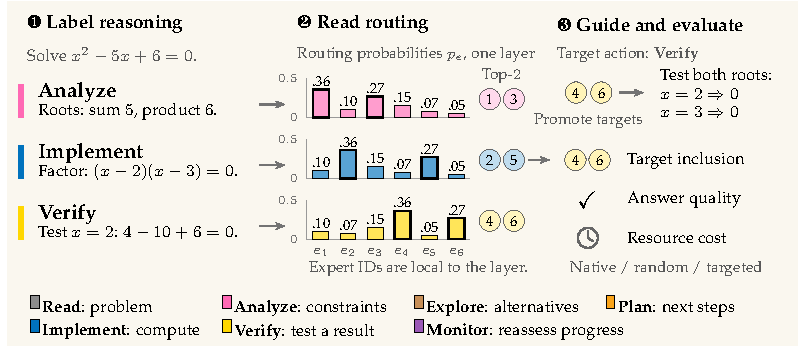
\includegraphics[width=\linewidth]{figures/journal/overview.pdf}
\caption{Reasoning states and routing probabilities in a constructed six-expert example.
%
Dark outlines and circled IDs identify the top-2 experts.
%
The seven-state key connects sentence function to color.
%
Promoting a Verify target set illustrates a checking continuation, whose target engagement, answer quality, and resource cost require separate evaluation.
%
Probabilities and text are explanatory examples, not measured effects.}
\label{fig:overview}
\end{figure}

Existing approaches regulate reasoning length through generation budgets or modify hidden representations to favor particular behaviors~\citep{muennighoff2025s1,chen2025seal,eisenstadt2025overclocking}.
%
Expert steering provides a complementary mechanism by promoting or suppressing behavior-associated experts~\citep{fayyaz2025steermoe}.
%
Online rerouting instead adapts selection scores to the available context~\citep{su2026rewiring}.
%
These approaches establish useful control interfaces, but they do not make every activity-associated route a beneficial intervention.
%
An expert may correlate with checking because it processes characteristic words.
%
Promoting it may change the route without producing a substantive check.
%
Answer quality and computational cost must therefore accompany the behavioral measurement.
%

We study routing interventions through a sequence of connected questions.
%
First, do expert selections contain information about a reasoning state beyond the text that expresses it?
%
Second, how do these states recur and transition, and does routing anticipate the next state?
%
Third, can a state-aware allocation preserve less frequent activities under a limited expert budget?
%
Finally, does activating or deactivating the experts nominated for a state move the reasoning toward or away from that state, and does it shorten the solution at retained accuracy?
%
We use mathematical reasoning as the evaluation setting and analyze eight MoE LLMs with separate controls for these questions.
%
The annotation vocabulary describes the visible function of a sentence.
%
It does not assume that an expert implements a dedicated cognitive operation.
%

Our contributions are the following.
%
\begin{enumerate}
\renewcommand{\labelenumi}{\circnum{\arabic{enumi}}}
\item We connect native expert allocation to interpretable reasoning states using held-out families and text-controlled readouts.
%
Routing adds state information in every analyzed model, supplying a measured basis for investigating state-conditioned interventions.
%
\item We characterize state occupancy, transitions, and duration across the eight models, distinguishing continued execution from returns to a state.
%
The next-state readouts in GPT-OSS and Qwen3.6 test whether routing anticipates a subsequent activity.
%
\item We compare expert retention under a fixed budget, where state balancing improves minimum native coverage in six models and reduces it in two.
%
\item We test state-conditioned routing edits in 29,377 paired continuations from frozen prefixes, with matched random controls and a pre-registered link to native solution length.
%
Activation and deactivation change neither the subsequent reasoning state nor the generated tokens and accuracy beyond matched random edits, although native states such as verification precede shorter remaining reasoning.
%
\end{enumerate}

Routing offers an intervention point within the computation of an LLM.
%
Our results show that it records which reasoning activity is under way, while brief edits to the experts associated with an activity leave the reasoning and its cost unchanged.
%

\section{Related Work}
\label{sec:related-work}

\paragraph{Sparse expert routing and expert specialization}
Sparsely gated mixture-of-experts layers let a trainable gate select a few feed-forward experts for each token, which increases model capacity without activating every parameter~\citep{shazeer2017moe}.
%
Switch Transformers simplify this routing and reduce its communication and computational cost at scale~\citep{fedus2022switch}.
%
Analyses of trained routers describe what these selections follow.
%
In OpenMoE, routing depends predominantly on token identity and changes little with context~\citep{xue2024openmoe}.
%
Across domains, a compact and largely domain-invariant group of experts receives most of the routing mass, including in architectures with shared experts~\citep{wang2026illusion}.
%
Selected expert sets also retain much of the input itself, since a sequence decoder trained on them reconstructs most tokens of the original text~\citep{nuriyev2026selections}.
%
These findings make routing an observable record of the processed text.
%
Whether expert selections add information about the function of a reasoning sentence beyond the words that express it remains an open question.
%
Our readouts address it by measuring the state information that routing adds to text baselines on held-out problem families.
%

\paragraph{Reasoning states and their dynamics}
Schoenfeld's episode theory describes mathematical problem solving as a sequence of functional episodes, such as reading, analysis, exploration, planning, implementation and verification~\citep{schoenfeld1985mathematical}.
%
\citet{li2025schoenfeld} adapt this vocabulary to seven sentence-level labels for DeepSeek-R1 solutions and report recurring transitions between them.
%
ThinkARM applies the same functional labels to traces from diverse models and finds reproducible dynamics that separate reasoning from non-reasoning models~\citep{li2026thinkarm}.
%
Representation-based analyses define states from the hidden activations instead.
%
Clustered step representations form reasoning graphs whose cycles and diameter grow in distilled reasoning models~\citep{minegishi2025topology}, and spectral step representations can be clustered into latent states whose transitions follow a first-order Markov chain~\citep{yu2025stateaware}.
%
Trajectory geometry also carries outcome signals: correct and incorrect mathematical solutions diverge at late steps~\citep{sun2026trajectories}, and frequent switching between lines of thought accompanies incorrect answers~\citep{wang2025thoughts}.
%
In sparse models, routes taken at fixed token anchors distinguish contexts well enough to select among completed rollouts~\citep{chen2026same}.
%
The state definitions of these approaches need not coincide, since a latent cluster may contain several functions and one function may occupy several clusters.
%
They describe the order and recurrence of reasoning activities without identifying the components that produce them.
%
We retain the explicit functional vocabulary and relate it to the experts selected at each layer, for both the current and the next state.
%

\paragraph{Readouts and causal evidence}
Probing classifiers estimate what a representation encodes, but their interpretation depends on the chosen baselines and remains correlational~\citep{belinkov2022probing}.
%
Conditional probing measures the information that a representation adds beyond a specified baseline representation~\citep{hewitt2021conditional}.
%
Decodable information need not be used by the model.
%
Amnesic interventions show that linguistic properties recoverable from BERT representations can be irrelevant to its predictions~\citep{elazar2021amnesic}, and causal-tracing localization of a stored fact does not identify the layer where an edit overrides it most effectively~\citep{hase2023localization}.
%
AxBench likewise evaluates concept detection and steering as distinct capabilities, and sparse-autoencoder features are not competitive on either~\citep{wu2025axbench}.
%
The visible trace has a similar limitation, because biasing features of the input can change chain-of-thought answers without being mentioned in the explanation~\citep{turpin2023language}.
%
Functional labels therefore characterize the visible text of a reasoning sentence.
%
For MoE models, \citet{chen2026beyond} reconstruct a reasoning-state readout from native routing and report router edits that change reasoning in the predicted direction.
%
These results separate two claims that a routing study can make.
%
A held-out readout beyond text establishes an association between experts and states, whereas control requires an edit whose effect exceeds that of equally sized unrelated edits.
%
Our design evaluates the two claims separately.
%

\paragraph{Steering reasoning through representations}
Activation steering modifies intermediate representations while preserving the model parameters.
%
Contrastive Activation Addition averages the activation differences between paired positive and negative examples and adds the resulting direction during generation~\citep{rimsky2024caa}.
%
Applied to thinking models, such directions modulate backtracking and expressions of uncertainty~\citep{venhoff2025steering}.
%
SEAL distinguishes execution, reflection and transition thoughts and calibrates reasoning with a training-free representation intervention~\citep{chen2025seal}, while sparse-autoencoder features selected for individual reasoning strategies provide strategy-level control~\citep{fang2026controllable}.
%
Efficiency-oriented interventions target the duration of reasoning.
%
Overclocking manipulates a representation of progress through the thinking phase~\citep{eisenstadt2025overclocking}, and Manifold Steering projects an overthinking direction onto a low-dimensional activation manifold~\citep{huang2025manifold}.
%
Local-geometry methods replace a single global direction with regions and within-region variation, represented by a mixture of factor analyzers~\citep{shafran2026regions}.
%
The reliability of these interventions varies.
%
Steering effects differ across inputs, and some concepts are brittle under reasonable prompt changes~\citep{tan2024reliability}.
%
Across 36 models from 14 families, the effects of the same steering methods vary widely, with no improvement or degraded performance in some models~\citep{silva2025offcourse}.
%
Expert edits act on a discrete part of the computation, namely the set of experts that process a token.
%
They require no assumption that a reasoning state corresponds to one linear feature or that an expert implements only one function.
%

\paragraph{Expert-level control and rerouting}
Sparse architectures make the participation of each expert an accessible intervention point.
%
SteerMoE nominates behavior-associated experts from activation differences between contrasting inputs and changes safety and faithfulness outcomes by activating or deactivating them at inference time~\citep{fayyaz2025steermoe}.
%
RICE selects experts that co-occur with thinking markers and reports that amplifying as few as two of them increases reasoning depth and efficiency on mathematical and scientific benchmarks~\citep{wang2025rice}.
%
Other methods act on the router as a whole.
%
Counterfactual routing analysis compares native routes with equal-compute alternatives on verified reasoning trajectories~\citep{yoon2026misrouted}, and continuous rerouting adapts additive router-logit vectors online from self-supervision on the current context~\citep{su2026rewiring}.
%
THESIS-MoE instead localizes sycophancy across model components and edits activations conditionally where the behavior is present~\citep{hassani2026thesismoe}.
%
Causal audits qualify associations of this kind.
%
In three MoE models, observational routing metrics fail to predict which experts matter under token-level ablation~\citep{engmann2026observation}.
%
In a pre-registered test of one frontier MoE with size-matched random-expert controls, only one of six routing-defined expert families meets a robust selectivity criterion, although the others also have causal effects~\citep{salomone2026modular}.
%
The steering methods target behaviors such as safety, faithfulness or reasoning depth, while the audits show that an association with routing need not imply selective control.
%
We test fine-grained reasoning states as targets and report each edit against native routing and against matched random experts.
%

\paragraph{Efficient reasoning and expert compression}
A longer trace spends more computation, but its additional steps can repeat a solution or explore alternatives with little effect on the answer.
%
\citet{chen2025overthinking} characterize this redundancy through outcome and process efficiency and use self-training to favor more concise solutions.
%
Budget forcing in s1 controls the duration of reasoning by terminating generation or extending it when the model attempts to finish~\citep{muennighoff2025s1}.
%
STACK assesses each step for uncertainty and redundancy and switches between compression strategies accordingly~\citep{sui2026think}.
%
These methods change how much reasoning is produced, and their evaluation makes the cost of an intervention part of the outcome.
%
Compression methods alter the executable model for efficiency and use different quantities to rank experts.
%
Post-training expert pruning can select, layer by layer, the expert combination that minimizes token reconstruction loss and add dynamic expert skipping~\citep{lu2024naee}, EAC-MoE prunes rarely selected experts~\citep{chen2025eac}, and REAP ranks experts by router gate values and expert activation norms~\citep{lasby2026reap}.
%
Coverage-maximized pruning allocates a global budget by attribution-guided channel scores within experts~\citep{ding2026coverage}.
%
Frequency criteria count participation and output-aware criteria estimate contribution, while class balancing gives rarely observed reasoning states equal influence on selection.
%
We compare class balancing with frequency and random selection under common expert budgets, scoring the coverage of held-out native selected slots for the least-covered state.
%
This endpoint describes which activities a keep-set retains, whereas physically removing experts also changes routing and the resulting solutions.
%
A routing edit can likewise save generated tokens, but it does not by itself reduce the experts held in memory.
%

\section{Reasoning Guidance through Routing Interventions}
\label{sec:method}

\subsection{Reasoning states and native expert selections}

We relate the visible function of a reasoning sentence to the experts selected by an MoE LLM while its tokens are processed.
%
The state vocabulary $\mathcal C$ contains Read, Analyze, Explore, Plan, Implement, Verify, and Monitor.
%
Read concerns the problem statement, Analyze interprets its constraints, Explore considers alternatives, and Plan organizes subsequent work.
%
Implement carries out a proposed calculation or construction, Verify checks a result, and Monitor assesses progress or the need to revise the approach.
%
The annotation instrument assigns these labels to generated text.
%
They provide observed targets for our analysis.
%

Let $y_s$ denote the assigned class of sentence $s$, and let $T_s$ be its token positions.
%
At routed layer $\ell$ and token $t$, the native selector executes the expert set $S_{\ell,t}$ of size $k_\ell$.
%
An expert identity includes model, layer, and local expert index.
%
For an observed token window $W$, its inclusion frequency is
\begin{equation}
 f_{\ell e}(W)=\frac{1}{|W|}\sum_{t\in W}
 \mathbf{1}\{e\in S_{\ell,t}\}.
 \label{eq:inclusion}
\end{equation}
Each inclusion frequency is between zero and one, and the frequencies sum to $k_\ell$.
%
Dividing them by $k_\ell$ yields a selected-slot distribution over experts.
%
This representation differs from the weights used to combine expert outputs, which may reflect normalization, learned scaling, or a shared-expert path.
%

The architecture's own selection rule defines the native routes.
%
Softmax and sigmoid scores, correction biases, grouped selection, and shared experts can all affect which identities are selected or how their outputs contribute.
%
We therefore compare information and coverage within a model before comparing the resulting summaries across models.
%
We do not align expert indices across models.
%

\subsection{Conditioning routing on a desired reasoning state}
\label{sec:conditioning}

We study expert inclusion and exclusion as interventions on the allocation made by the router.
%
A target set $K_{\ell,c}$ contains $n$ layer-local experts nominated for a reasoning activity $c$ on the training families of the evaluation fold.
%
Nomination ranks experts by their inclusion excess for class $c$ over the other classes, and each class and fold uses the single layer whose nominated set has the largest training association, with stability across training subsamples breaking ties.
%
Activity association alone does not certify that the targets cause it.
%

Let $h_{\ell,t}$ be the layer input at token position $t$, and let $R_\ell$ denote the native router's affinity computation.
%
We write the affinities, the selection priorities, and the native top-$k_\ell$ selection as
\begin{equation}
 q_{\ell,t}=\phi\big(R_\ell(h_{\ell,t})\big),\qquad
 \pi_{\ell,t}=q_{\ell,t}+b_\ell,\qquad
 S_{\ell,t}=\operatorname{top}_{k_\ell}(\pi_{\ell,t}),
 \label{eq:routing-scores}
\end{equation}
where $\phi$ is the model's softmax or sigmoid scoring and $b_\ell$ its selection-correction bias, zero when the router has none.
%
At a frozen prefix ending immediately before $t_0$, the pulse $g_t=\mathbf{1}\{t_0\leq t<t_0+P\}$ covers the states that predict the first $P$ generated tokens.
%
During the pulse, activation and deactivation replace the selected identities by
\begin{equation}
 \widetilde S^{+}_{\ell,t}=K_{\ell,c}\cup\operatorname{top}_{k_\ell-n}\big(\pi_{\ell,t}\big|_{\mathcal E\setminus K_{\ell,c}}\big),\qquad
 \widetilde S^{-}_{\ell,t}=\operatorname{top}_{k_\ell}\big(\pi_{\ell,t}\big|_{\mathcal E\setminus K_{\ell,c}}\big),
 \label{eq:conditioning}
\end{equation}
where $\mathcal E$ is the set of experts at layer $\ell$.
%
The combination weights of the new selection are the native affinities $q_{\ell,t}$ of its members, renormalized and scaled exactly as the native router does.
%
Outside the pulse, at other layers, and after reasoning closes, routing is native.
%
The edit therefore keeps the selection budget $k_\ell$ and the expert-combination rule, and it changes only which experts compute the pulse tokens.
%

\begin{figure}[tb]
\centering
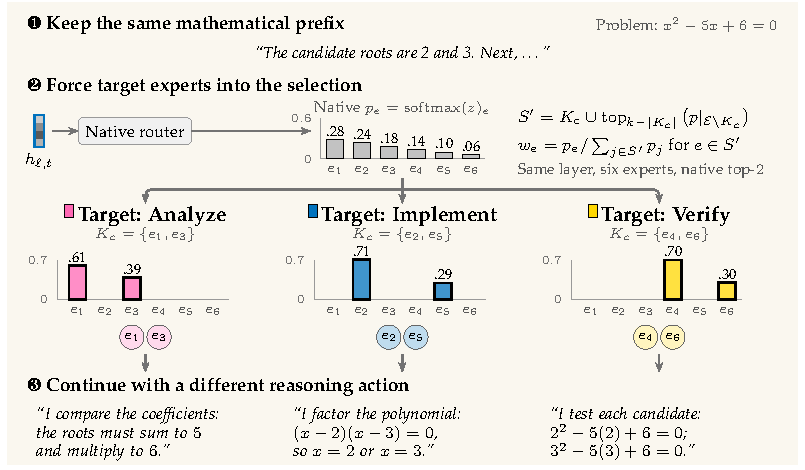
\includegraphics[width=\linewidth]{figures/journal/conditioning.pdf}
\caption{Three class-characteristic continuations from one mathematical prefix.
%
In this constructed softmax example, activation places the indicated expert pair in the top-2 selection and renormalizes their native probabilities.
%
Colored bars and circled IDs identify the top-2 experts.
%
The Analyze, Implement, and Verify continuations illustrate the intervention hypothesis, not measured semantic control.
%
The selection budget and expert-combination rule are retained.}
\label{fig:conditioning}
\end{figure}

The intervention size is the central count $n=\lceil k_\ell/2\rceil$, and the pulse length $P$ is the training median sentence length in tokens.
%
A matched random control replaces $K_{\ell,c}$ by $n$ experts of the same layer drawn from the same native-frequency quintiles and disjoint from every nominated set.
%
Each prefix receives one native continuation and, for every class, targeted activation, targeted deactivation, and the two matched random controls.
%
Comparing a targeted arm with its matched control tests the nominated identities, and comparing either arm with native routing tests the edit itself.
%
All arms of one prefix use the same sampler and seed, and every continuation runs to its natural end or to the original generation allowance.
%
The reasoning state after the edit is read from the first complete sentence and from class occupancy over the next $16\,Q_{75}$ tokens, where $Q_{75}$ is the training upper-quartile sentence length.
%
A lexical classifier trained on the judge-labelled native sentences of the other folds assigns these classes, so no intervention output is relabelled by the judge (Appendix~\ref{app:lexical-readout}).
%
Efficiency is measured by the generated tokens to a final answer and by strict answer accuracy.
%

\subsection{Steering expert selection throughout reasoning}
\label{sec:whole-steering}

A pulse tests whether a local edit redirects the next sentence.
%
Expert steering in MoE LLMs instead fixes expert participation over the whole generation~\citep{fayyaz2025steermoe}.
%
We therefore also steer expert selection at every prompt and reasoning token, from the first prompt token until the reasoning closes, and leave the final answer to native routing.
%

Whole-reasoning steering promotes or suppresses a reasoning activity $c$ through a set $A_c$ of activated and a set $D_c$ of deactivated layer--expert pairs.
%
Nomination uses the inclusion risk difference $\Delta_{\ell,e,c}$, the rate at which expert $e$ of layer $\ell$ is selected on sentences of class $c$ minus its rate on sentences of the other classes, estimated on the training families of each fold and retained only when its sign is stable across subsample refits.
%
Promoting $c$ activates the pairs with the largest positive differences and deactivates those with the most negative ones, whereas suppressing $c$ deactivates the pairs with the largest positive differences.
%
Nominations range over all MoE layers, so a single edit can change many layers at once.
%

At a steered position, the override follows SteerMoE~\citep{fayyaz2025steermoe}.
%
For a softmax router with log-probabilities $s_{\ell,t}=\log q_{\ell,t}$, an activated expert receives $\max_e s_{\ell,t,e}+\epsilon$ and a deactivated expert $\min_e s_{\ell,t,e}-\epsilon$ before the native top-$k_\ell$ selection and renormalization.
%
For a sigmoid router with selection biases, an activated expert takes the affinity $\sigma(\max_e z_{\ell,t,e}+\epsilon)$ of the largest router logit $z_{\ell,t}$ and is always selected, a deactivated expert is never selected, and the combination weights are renormalized and scaled as natively.
%
We use $\epsilon=0.01$, and every layer activates fewer than $k_\ell$ experts and keeps at least $k_\ell$ selectable ones, so the selection budget of Equation~\eqref{eq:routing-scores} is preserved.
%

The edit size follows the counts published for SteerMoE~\citep{fayyaz2025steermoe}.
%
GPT-OSS-20B promotes with 10 activated and 50 deactivated pairs and suppresses with 20 deactivated pairs, and the Qwen models promote with 15 activated pairs and suppress with 500 deactivated pairs.
%
Each other model receives the same share of its own pairs, scaling activation counts by its number of MoE layers and deactivation counts by its number of layer--expert pairs, relative to the 48 layers and 128 experts of Qwen3-30B-A3B.
%
Full, half and quarter strength edit $\lceil f\,n\rceil$ pairs for $f\in\{1,\tfrac12,\tfrac14\}$ and each published count $n$.
%

The direction of each edit comes from the native association between reasoning states and the remaining solution length (Appendix~\ref{app:efficiency-link}).
%
Classes whose sentences precede shorter remaining reasoning at the same question and position are promoted, and classes that precede longer remaining reasoning are suppressed.
%
Each model uses its own pre-registered association, except LFM2.5, whose native association was not part of the pre-registration and which therefore uses the signs pooled across the other models.
%
A matched random control edits the same number of pairs at the same layers, with the same role and from the same native-frequency quintiles, disjoint from the target and from the nominations of the opposite direction.
%
A targeted-minus-random contrast therefore tests the nominated identities at a fixed edit size and placement.
%

Efficiency is the reduction in $\log(1+T)$, where $T$ counts the tokens until the reasoning closes, together with the change in strict accuracy.
%
Steering is efficient when the simultaneous lower bound of the token reduction exceeds zero and the accuracy change stays above $-5$ percentage points.
%
The lexical readout of Appendix~\ref{app:lexical-readout} also measures the share of reasoning tokens in each state, testing whether a promoted state grows and a suppressed state shrinks.
%

\subsection{Incremental information about the present state}
\label{sec:present-method}

The present-state task predicts $y_s$ from the same text context available to the annotation reader.
%
Its baseline representation $x_s$ includes the available previous, current, and next sentences, token identity, position, and sentence length.
%
The routing-augmented representation additionally includes $r_s$, a summary of the sentence's expert allocations.
%
Both classifiers use the same outer evaluation families and the same label targets.
%

Let $a_{\ell,t}$ denote the top-1 expert at layer $\ell$ and token $t$.
%
The sentence histogram and assembled routing vector are
\begin{equation}
\begin{aligned}
 h^{(1)}_{s,\ell e}&=\frac{1}{|T_s|}\sum_{t\in T_s}
 \mathbf{1}\{a_{\ell,t}=e\},\\
 r_s&=Z_{\mathcal T}\!\left(
 D_s\mathbin{\Vert}R_s\mathbin{\Vert}
 P_{\mathcal T}(h^{(1)}_s-\mu_{\mathcal T})\right).
\end{aligned}
\label{eq:present-features}
\end{equation}
Here $\Vert$ concatenates features.
%
The histogram is flattened across layers and experts.
%
Its training mean $\mu_{\mathcal T}$ and principal component projection $P_{\mathcal T}$ are fitted within the training fold.
%
$D_s$ measures depth-path surprise and $R_s$ temporal persistence.
%
$Z_{\mathcal T}$ standardizes each coordinate using that fold's mean and standard deviation.
%
Appendix~\ref{app:readout-features} defines these components and the retained numerical settings.
%

The multinomial ridge readout assigns class probabilities to $v_s$ as
\begin{equation}
 p_{B,b}(c\mid v_s)=
 \frac{\exp(B_{\cdot c}^{\top}v_s+b_c)}
 {\sum_{j\in\mathcal C}\exp(B_{\cdot j}^{\top}v_s+b_j)}.
 \label{eq:readout-map}
\end{equation}
Here $B$ contains one coefficient column per class and $b$ is the intercept vector.
%
For either $v_s=x_s$ or $v_s=[x_s;r_s]$, the fitted parameters minimize
\begin{equation}
 (\widehat B,\widehat b)=\operatorname*{arg\,min}_{B,b}
 \left\{-\frac{\sum_{s\in\mathcal T}w_s\log p_{B,b}(y_s\mid v_s)}
 {\sum_{s\in\mathcal T}w_s}
 +\frac{\lambda}{2}\|B\|_F^2\right\}.
 \label{eq:readout-fit}
\end{equation}
The training sentences $\mathcal T$ receive weights $w_s$ that give each question equal total weight.
%
The penalty leaves the intercept unpenalized.
%
Separate fits for the two inputs give the held-out probability vectors
\begin{equation}
 \begin{aligned}
 \widehat p_x(s)&=
 \bigl(p_{\widehat B_x,\widehat b_x}(c\mid x_s)\bigr)_{c\in\mathcal C},\\
 \widehat p_{x,r}(s)&=
 \bigl(p_{\widehat B_{x,r},\widehat b_{x,r}}(c\mid[x_s;r_s])\bigr)_{c\in\mathcal C}.
 \end{aligned}
 \label{eq:present-predictions}
\end{equation}
All feature transforms and parameter estimates use the corresponding training fold.
%
Setup gives the regularization-selection procedure.
%

We name the held-out reduction in cross-entropy \emph{routing information gain} (RIG).
%
This diagnostic measures how much routing adds to the text baseline when identifying the present state.
%
For text predictions $\widehat p_x$ and routing-augmented predictions $\widehat p_{x,r}$,
\begin{equation}
 \mathrm{RIG}
 =\mathcal L(\widehat p_x,y)-\mathcal L(\widehat p_{x,r},y).
 \label{eq:readout}
\end{equation}
RIG is measured in nats per sentence and can take either sign, with no finite universal bound.
%
Positive RIG supports incremental state information.
%
Loss first averages labelled sentences within a question, then questions receive equal total weight.
%
All training, tuning, and test splits keep duplicate families together.
%

A lexical null preserves the token identities and absolute-position strata used by the control while permuting routing paths within those strata.
%
Repeating the same readout procedure with these paths tests whether the gain depends on the original alignment between routing and reasoning labels.
%
The alignment gain subtracts the observed routing-augmented loss from the mean lexical-null loss.
%
It is measured in nats per sentence and is unbounded in either direction.
%
Positive values support information carried by the original routing alignment.
%
This is a retrospective label-information test because the current and following sentence text are available to the baseline.
%

\subsection{Prediction before the destination sentence}
\label{sec:next-method}

Next-state prediction uses routing from the source sentence to predict the class of its originally adjacent destination.
%
The baseline observes previous and source-sentence text, lexical controls and earlier class history, together with a training-only estimate of the current class.
%
Let $u_s$ collect these baseline features.
%

For this task, $W_s$ contains the last $\min(16,|T_s|)$ owned tokens of the source sentence.
%
Its selected-slot histogram is $h^{(16)}_{s,\ell e}=f_{\ell e}(W_s)/k_\ell$.
%
Training sentences define a marginal routing profile $\pi^0$ and a profile $\pi^c$ for each reasoning class $c$, as detailed in Appendix~\ref{app:next-state}.
%
Their log ratios give seven routing scores and the next-state feature vector
\begin{equation}
\begin{aligned}
 d_{s,c}&=\frac{1}{L}\sum_{\ell=1}^{L}\sum_e
 h^{(16)}_{s,\ell e}\log\frac{\pi^0_{\ell e}}{\pi^c_{\ell e}},\\
 r_s^{\mathrm{next}}&=Z_{\mathcal T}\!\left((d_{s,c})_{c\in\mathcal C}\right).
\end{aligned}
\label{eq:next-features}
\end{equation}
Here $L$ is the number of routed layers.
%
The profiles and coordinate standardization use only the corresponding training fold.
%
Each raw score is a convex average of finite log ratios and can have either sign.
%
For fixed profiles, its bounds are
\begin{equation}
 \frac{1}{L}\sum_{\ell}\min_e\log\frac{\pi^0_{\ell e}}{\pi^c_{\ell e}}
 \;\leq d_{s,c}\leq\;
 \frac{1}{L}\sum_{\ell}\max_e\log\frac{\pi^0_{\ell e}}{\pi^c_{\ell e}}.
\end{equation}
Coordinate standardization subsequently centers and rescales these scores.
%
They summarize all selected slots, separately from the present-state top-1 representation.
%
Both $u_s$ and $r_s^{\mathrm{next}}$ are available before the destination sentence begins.
%
The same multinomial ridge map is fitted separately to $u_s$ and $[u_s;r_s^{\mathrm{next}}]$, using $y_{s+1}$ as the training target and equal total weight per question.
%
Its held-out predictions are
\begin{equation}
 \begin{aligned}
 \widehat p_{\mathrm{past}}(s)&=
 \bigl(p_{\widehat B_{\mathrm{past}},\widehat b_{\mathrm{past}}}(c\mid u_s)\bigr)_{c\in\mathcal C},\\
 \widehat p_{\mathrm{past},r}(s)&=
 \bigl(p_{\widehat B_{\mathrm{past},r},\widehat b_{\mathrm{past},r}}
 (c\mid[u_s;r_s^{\mathrm{next}}])\bigr)_{c\in\mathcal C}.
 \end{aligned}
 \label{eq:next-predictions}
\end{equation}
The current-class estimate itself uses grouped out-of-fold predictions within the training population.
%
The reported losses average held-out log losses across the original repeated fold assignments.
%
The \emph{anticipatory routing gain} (ARG) for the next assigned label is
\begin{equation}
 \mathrm{ARG}=\mathcal L(\widehat p_{\mathrm{past}},y_{s+1})
 -\mathcal L(\widehat p_{\mathrm{past},r},y_{s+1}).
 \label{eq:anticipation}
\end{equation}
ARG is measured in nats per adjacent pair.
%
Positive values support information about a state before its sentence begins.
%
Its range is unbounded in either direction, as for RIG.
%
These names identify the claim and information set of each diagnostic, while both retain the original held-out log-loss estimator.
%

Original sentence indices and reasoning segments determine adjacency.
%
A missing label or a sentence gap breaks the sequence.
%
We retain these breaks instead of connecting the nearest available labels.
%
A source-length sensitivity retains sentences with at least 32 tokens.
%
The routing window already stays inside its source sentence in both conditions.
%
The restriction ensures a full 16-token window and changes the supported population.
%
Present-state and next-state prediction consequently have different information sets and different support.
%

\subsection{Class-balanced expert retention}
\label{sec:selection-method}

The allocation analysis learns a keep-set $K_\ell$ from training families and measures how well it contains held-out native selections.
%
All candidate experts belong to the model's layer-local pool.
%
The methods share the same identity budget $b_\ell$, the same layer and group quotas, and the same training data.
%
Expert ranking uses labelled allocation counts without correctness information.
%

For training family $f$, class $c$, layer $\ell$, and expert $e$, let $C_{fc\ell e}$ be the selected-slot count averaged over the family's member questions.
%
Class balancing normalizes within family and class, averages supported families, then weights classes equally:
\begin{equation}
 s^{\mathrm{bal}}_{\ell e}
 =\frac{1}{|\mathcal C|}\sum_{c\in\mathcal C}
 \frac{1}{|\mathcal F_c|}\sum_{f\in\mathcal F_c}
 \frac{C_{fc\ell e}}{\sum_jC_{fc\ell j}}.
 \label{eq:balanced-selection}
\end{equation}
Here $\mathcal F_c$ contains training families with observed class $c$.
%
Every class must have training support.
%
The normalized scores lie between zero and one.
%
This estimator gives a class equal weight regardless of how much labelled token mass it contributes.
%

The frequency control pools the same labelled counts:
\begin{equation}
 s^{\mathrm{freq}}_{\ell e}
 =\frac{\sum_{f,c}C_{fc\ell e}}{\sum_{f,c,j}C_{fc\ell j}}.
 \label{eq:frequency-selection}
\end{equation}
The methods rank experts by their corresponding training score, apply the common quotas, and break ties by original expert ID.
%
A fixed random selector supplies a third allocation control.
%
Its priorities are independent of the class counts and remain fixed during the comparison.
%

For a held-out family, class, and layer, retained coverage is the fraction of its native selected slots whose expert belongs to $K_\ell$.
%
We average family-weighted coverage equally over routed layers for each class.
%
We call the minimum \emph{weakest-state coverage} (WSC):
\begin{equation}
 \mathrm{WSC}(K)=100\min_{c\in\mathcal C}R_c(K).
 \label{eq:min-coverage}
\end{equation}
WSC ranges from 0 to 100\% and measures whether the retained expert budget contains the native selections of every reasoning activity.
%
The paired \emph{coverage gain},
\begin{equation}
 \Delta\mathrm{WSC}=\mathrm{WSC}(K_{\mathrm{bal}})
 -\mathrm{WSC}(K_{\mathrm{freq}}),
 \label{eq:coverage-gain}
\end{equation}
ranges from $-100$ to $100$ percentage points.
%
Positive values support class balancing for the least-covered activity at the same expert budget.
%
The per-class denominator includes observed labelled selections only.
%
The retained-slot fraction measures containment of the original routes.
%
Rerouting after removal can change the generated solution.
%

\subsection{State distributions and temporal summaries}
\label{sec:dynamics-method}

State occupancy describes how the observed labelled tokens are distributed across the seven classes.
%
For an attempt, class $c$ has occupancy equal to its labelled token count divided by the total labelled token count.
%
Label coverage uses total completion tokens as its denominator.
%
Reporting both prevents a heavily sampled state distribution from being read as full-trace annotation.
%

Within an uninterrupted labelled segment, next-class probabilities use only observed adjacent sentence boundaries.
%
Consecutive sentences with the same class form an observed dwell run.
%
Gaps and the start or end of an observed segment censor the run.
%
These measurements describe the available annotated trajectory.
%
For the native distribution summaries, repeats first average within a benchmark--family occurrence, families average within each benchmark, and the benchmarks receive equal weight.
%

Uncertainty follows the original procedure for each study.
%
Family resampling retains within-family dependence, while the conditional distribution of a fixed fitted readout or selected keep-set omits variation from refitting.
%
We report the scope of each simultaneous correction with its result rather than treating separately constructed panels as one joint test.
%

\section{Experimental Setup}
\label{sec:setup}

\subsection{Models and routing geometry}

Table~\ref{tab:models} lists the eight evaluated models.
%
Each evaluated model retains its native router, tokenization, reasoning format, and shared-expert behaviour.
%
The observed number of routed layers excludes dense feed-forward blocks.
%
LFM2.5 has 24.0 billion total and 2.45 billion active parameters according to its release card, which advertises a 131,072-token context.\footnote{\url{https://huggingface.co/LiquidAI/LFM2.5-24B-A2B}}
%

\begin{table}[tb]
\centering\small
\caption{Models, routing geometry, and native execution profiles.
%
$L$ counts routed layers, $E$ experts per layer, and $k$ experts selected per token.
%
Context gives the native context capacity used for generation, in tokens.}
\label{tab:models}
\setlength{\tabcolsep}{4pt}
\begin{adjustbox}{max width=\linewidth}
\begin{tabular}{@{}lrrrr@{}}
\toprule
& \multicolumn{3}{c}{Routing geometry} & \\
\cmidrule(lr){2-4}
Model & $L$ & $E$ & $k$ & Context \\
\midrule
\modelname{openai}{GPT-OSS-20B} & 24 & 32 & 4 & 131,072 \\
\modelname{nvidia}{Nemotron-3.5-Lightning-30B-A3B} & 23 & 128 & 6 & 133,120 \\
\modelname{qwen}{Qwen3.5-35B-A3B} & 40 & 256 & 8 & 133,120 \\
\modelname{qwen}{Qwen3.6-35B-A3B} & 40 & 256 & 8 & 133,120 \\
\modelname{gemma}{Gemma-4-26B-A4B} & 30 & 128 & 8 & 133,120 \\
\modelname{zhipu}{GLM-4.7-Flash (30B-A3B)} & 46 & 64 & 4 & 133,120 \\
\modelname{qwen}{Qwen3-30B-A3B} & 48 & 128 & 8 & 40,960 \\
\modelname{liquid}{LFM2.5-24B-A2B} & 38 & 64 & 4 & 131,072 \\
\bottomrule
\end{tabular}
\end{adjustbox}
\end{table}

The evaluated weight formats are MXFP4 for GPT-OSS, NVFP4 for Nemotron and Gemma, GPTQ-Int4 for Qwen3.5, FP8 for Qwen3.6, and BF16 for GLM, Qwen3-30B, and LFM2.5.
%

The card-profile mathematical evaluation uses each model's own decoding settings.
%
Qwen3.5 and Qwen3.6 use temperature 1, top-$p$ 0.95, top-$k$ 20, and presence penalty 1.5.
%
Nemotron and GLM use temperature 1 and top-$p$ 0.95.
%
Gemma uses temperature 1, top-$p$ 0.95, and top-$k$ 64 with thinking enabled.
%
Qwen3-30B uses temperature 0.6, top-$p$ 0.95, and top-$k$ 20.
%
GPT-OSS uses its retained temperature-1, top-$p$-1 profile with medium reasoning effort.
%
LFM2.5 uses its card profile of temperature 0.1, top-$k$ 50, and repetition penalty 1.05 with thinking enabled.
%
These profiles describe the generated workloads.
%
They provide within-model sources for the routing analyses, while cross-model score differences also reflect decoding and output budgets.
%

Each native benchmark request contains one user message, without a separate system instruction or worked examples.
%
The model's native chat template formats the request.
%
Appendix~\ref{app:native-prompt} gives the shared prompt and model-specific thinking settings.
%

\subsection{Benchmarks and independent evaluation units}

The retained suite follows the mathematical evaluation used by SPIRAL~\citep{liu2025spiral}.
%
The six benchmarks contain 30 AIME24 questions, 30 AIME25 questions, 40 AMC23 questions, 500 MATH-500 questions, 272 Minerva questions, and 675 OlympiadBench questions.
%
AIME24, AIME25, and AMC23 use 32 attempts per question.
%
The other benchmarks use one.
%
Each complete native evaluation therefore has 4,647 attempts on 1,547 questions.
%
MATH-500 uses the retained MATH evaluation subset associated with process-supervision evaluation~\citep{lightman2024verify}.
%
OlympiadBench contributes the retained mathematical subset~\citep{he2024olympiadbench}, and Minerva contributes quantitative reasoning problems~\citep{lewkowycz2022minerva}.
%

Question identity distinguishes benchmark and original source problem.
%
Near-duplicate questions form a shared family.
%
The full allocation population contains 1,486 families, whereas the common readout population contains 522 questions in 509 families.
%
Repeated answers, sentences, and token selections are measurements within these independent problem units.
%
They do not increase the number of independent questions.
%

% Adapted from SPSD tab:main-results and SYNCO tab:mainRes.
% Destination adaptation: SPSD grouped benchmark columns, SYNCO model icons and caption-only key; naturally sized body.
\begin{table}[tb]
\centering\small
\caption{Mean native mathematical accuracy (\%) under each model's card profile, with question-bootstrap 95\% confidence intervals as subscripts ($\pm$ the larger original one-sided margin).
%
Repeated attempts stay grouped by source question.
%
Scores condition on adjudicated attempts.
%
Bold and underline identify the largest and second-largest unrounded means within each benchmark, with ties sharing a rank.
%
Minerva and Olympiad denote Minerva Math and OlympiadBench.}
\label{tab:benchmarks}
\setlength{\tabcolsep}{1.5pt}
\begin{adjustbox}{max width=\linewidth}
\begin{tabular}{@{}lcccccc@{}}
\toprule
 & \multicolumn{3}{c}{Competition mathematics} & \multicolumn{3}{c}{Quantitative reasoning}\\
\cmidrule(lr){2-4}\cmidrule(lr){5-7}
Model & AIME24 & AIME25 & AMC23 & MATH-500 & Minerva & Olympiad \\
\midrule
\modelname{openai}{GPT-OSS-20B} & \cid{78.7}{13.0}{9.7} & \cid{76.0}{11.4}{10.0} & \cid{97.3}{2.7}{2.1} & \cid{97.0}{1.6}{1.4} & \cid{69.1}{5.9}{5.5} & \cid{83.2}{2.8}{2.7} \\
\modelname{nvidia}{Nemotron-3.5-Lightning-30B-A3B} & \cid{87.8}{12.5}{8.8} & \cid{87.2}{11.3}{9.2} & \secondcid{99.8}{0.3}{0.2} & \cid{98.8}{1.0}{0.8} & \cid{73.5}{5.9}{5.1} & \cid{88.6}{2.4}{2.4} \\
\modelname{qwen}{Qwen3.5-35B-A3B} & \secondcid{94.0}{8.6}{5.4} & \cid{88.3}{11.3}{9.8} & \bestcid{100.0}{0.0}{0.0} & \secondcid{99.4}{0.8}{0.6} & \cid{73.4}{5.5}{5.5} & \bestcid{92.3}{2.1}{2.1} \\
\modelname{qwen}{Qwen3.6-35B-A3B} & \bestcid{94.8}{7.1}{5.0} & \bestcid{89.7}{10.9}{9.2} & \bestcid{100.0}{0.0}{0.0} & \bestcid{99.6}{0.6}{0.4} & \secondcid{74.8}{5.6}{5.2} & \secondcid{92.0}{2.1}{1.9} \\
\modelname{gemma}{Gemma-4-26B-A4B} & \cid{90.8}{9.8}{7.2} & \cid{86.8}{10.5}{8.8} & \cid{99.7}{0.6}{0.3} & \cid{99.0}{1.0}{0.8} & \bestcid{75.6}{4.8}{5.2} & \cid{90.8}{2.2}{2.1} \\
\modelname{zhipu}{GLM-4.7-Flash (30B-A3B)} & \cid{93.2}{7.7}{4.9} & \secondcid{89.6}{9.7}{7.6} & \cid{99.4}{0.5}{0.4} & \cid{98.4}{1.2}{1.0} & \cid{73.1}{5.5}{5.2} & \cid{90.5}{2.2}{2.1} \\
\modelname{qwen}{Qwen3-30B-A3B} & \cid{80.2}{14.7}{11.0} & \cid{71.1}{13.3}{12.1} & \cid{97.7}{2.5}{1.8} & \cid{98.0}{1.2}{1.2} & \bestcid{75.6}{5.2}{4.8} & \cid{84.6}{2.8}{2.5} \\
\modelname{liquid}{LFM2.5-24B-A2B} & \cid{86.9}{12.3}{8.4} & \cid{84.4}{9.9}{8.6} & \cid{97.9}{2.3}{1.7} & \cid{98.8}{1.0}{0.8} & \cid{74.2}{5.7}{5.2} & \cid{89.0}{2.5}{2.2} \\
\bottomrule
\end{tabular}
\end{adjustbox}

\end{table}


Table~\ref{tab:benchmarks} describes the native mathematical workload.
%
Scores retain the source adjudication rule and unresolved answers.
%
Across the 37,176 assigned attempts, 34 answers remain unresolved.
%
The reported scores condition on adjudicated attempts.
%
Appendix~\ref{app:benchmark-details} supplies the per-cell scored denominators and original question-bootstrap intervals.
%
The separate historical fixed-budget generation corpus uses the same question roster with its original decoding and scoring rules.
%
We keep that corpus separate from the card-profile scores.
%

\subsection{Sentence annotation and captured populations}

The primary native-label corpus uses a frozen Qwen3.8-27B reader.
%
Its deployed profile has temperature 1, top-$p$ 0.95, top-$k$ 20, and a 16,384-token output budget, with low reasoning effort.
%
The same program and configuration annotate the eight model populations.
%
Each request supplies the mathematical problem and the available previous, current, and next sentence context.
%
Each assigned sentence receives one episode label.
%

The allocation population draws one retained attempt uniformly per question with seed 20260925.
%
It therefore samples one of the 32 competition attempts, while single-attempt questions contribute their sole retained solution.
%
Annotation first samples up to ten sentences from each selected attempt, then samples remaining sentences from the pooled selected attempts toward a nominal 100,000-sentence budget per model.
%
Sentences assigned through an overlapping outcome-stratified sample are also available.
%
Unassigned sentences and unusable reader outputs have no observed label.
%
The distributions and coverage estimates condition on the resulting labelled population.
%
Appendix~\ref{app:annotation} defines segmentation and token ownership.
%

The annotation instrument was developed using the released SAT responses of \citet{li2025schoenfeld} and prompt optimization with GEPA~\citep{agrawal2026gepa}.
%
The imported 40-example seed is compared with an optimized prompt on 407 development units.
%
Selection maximizes balanced accuracy while allowing no class's recall to fall by more than 0.10.
%
Plan recall falls from 0.750 to 0.563 under optimization, so the seed is selected.
%
The deployment check obtains 0.710 accuracy on 407 reused validation units.
%
Appendix~\ref{app:annotation} reports the selection and deployment evidence.
%
This external validation limits how strongly native generated-text labels can be interpreted.
%

The present-state readout uses the common 522-question population, with 31,902--38,931 labelled sentences per model.
%
Expert selection uses the full one-attempt-per-question allocation population and the original class-count archives.
%
The native-state distribution summaries use their own available sentence populations, with 1,486-family support in seven models and 509-family support in Qwen3.6.
%
The populations are specified separately because a larger expert-count archive does not imply an equally complete sentence-level trajectory.
%

\subsection{Readout fitting and uncertainty}

Present-state classification uses multinomial ridge readouts with five outer and three inner duplicate-family folds.
%
The text baseline retains token-identity features, position, sentence length, and the original reader-context text.
%
Routing adds top-1 expert histograms reduced to 64 components, depth-path surprise across adjacent layers, and temporal persistence across adjacent tokens, as defined in Appendix~\ref{app:readout-features}.
%
Learned transformations and regularization are fitted within the training folds.
%
Absent source text is never replaced by future text.
%
Appendix~\ref{app:readout} gives the feature transforms and regularization search.
%

We report each 95\% confidence interval $[L,U]$ as $\hat\theta\pm h$, with $h=\max(\hat\theta-L,U-\hat\theta)$.
%
Statistical comparisons use the original limits.
%

The original intervals use 5,000 whole-family bootstrap resamples and a model-specific seven-comparison correction.
%
Five lexical-null draws repeat the same fitting procedure after the declared routing permutation.
%
Next-state results retain their separate six-comparison correction and question-balanced estimand.
%
Present- and next-state intervals retain separate correction scopes.
%

The native-state summaries use 10,000 paired whole-family resamples.
%
Repeats average within each benchmark--family cell, families receive equal weight within a benchmark, and the six benchmarks receive equal weight.
%
The maximum centered standardized deviation supplies the simultaneous critical value within each model's native-dynamics panel.
%
An undefined resample or insufficient benchmark support leaves the affected interval unavailable.
%
These intervals do not estimate run-to-run variability.
%

\subsection{Retention budgets}

The retrospective retention comparison fixes 75\% of expert identities at every routed layer.
%
Its quotas are 24, 96, 192, 192, 96, 48, 96, and 48 experts for the eight evaluated models in Table~\ref{tab:models}.
%
Five common family folds determine training and evaluation.
%
Training sets overlap across these folds.
%
The random priorities use seed 20261008 and one fixed set per model, so the comparison conditions on those particular random sets.
%
Every evaluated fold has support for all seven reasoning classes.
%

\subsection{Intervention population and continuations}
\label{sec:intervention-setup}

The intervention study uses the 129 families of the held-out intervention cohort, balanced across benchmarks, family folds and thirds of solution progress.
%
In each family, a deterministic draw selects a labelled sentence boundary in the assigned third of a native solution, and the frozen prefix ends immediately before that sentence.
%
A family without a compatible boundary in its assigned third is not replaced, leaving 128 families in Nemotron and Qwen3-30B and 112 in LFM2.5.
%
Nominations, layer choices and median sentence lengths use only the training families of the prefix's fold.
%
The target size is two experts in GPT-OSS, GLM and LFM2.5, three in Nemotron, and four in the Qwen and Gemma models.
%
The pulse covers 13 to 20 tokens, and the analysis window covers 320 to 480 tokens, depending on the model and fold.
%

Each family receives one native continuation and, for each of the seven classes, targeted activation, targeted deactivation and their two matched random controls.
%
The eight models therefore contribute 29,377 continuations.
%
All arms of a family use the model's card sampler and the same seed.
%
Each continuation runs to its natural end or to the original completion allowance minus the prefix.
%
A request that is still running at the end of a compute allocation is resumed by passing its prompt, prefix and generated tokens through the same hooks, so the pulse remains at its original positions and no continuation is redrawn.
%
Answers use the strict scoring of the native evaluation.
%

Effects are paired differences within a family and class.
%
Each family first averages its classes, and its models for pooled estimates; families then receive equal weight within each benchmark, and benchmarks receive equal weight.
%
Intervals use 10,000 whole-family bootstrap resamples, with a simultaneous critical value for each declared family of contrasts.
%
The lexical readout that labels generated sentences is cross-fitted by family fold (Appendix~\ref{app:lexical-readout}).
%

\subsection{Whole-reasoning steering population}
\label{sec:whole-setup}

Whole-reasoning steering starts from the original benchmark prompt of each intervention family, so each model keeps its 129, 128 or 112 families.
%
At its base strength, each family receives a native continuation, a second native continuation with another seed, and a targeted and a matched random continuation for every cell, namely the promotion of each of the seven classes and the suppression of each class tied to longer reasoning.
%
The other two strengths run only the efficiency-directed cells, the promotion of classes tied to shorter reasoning and the suppression of classes tied to longer reasoning, and they share the native continuations of the base strength.
%
All continuations of a family share the prompt, the model's card sampler and the seed, except the repeated native one, whose difference from the first measures sampling variation.
%
The random experts are drawn separately at each strength to match its targets.
%
Every continuation receives the full completion allowance of the model card, and continuations still running at the end of the generation period are kept as unknown outcomes.
%

Before production, a check of 48 continuations from eight families per model compared steered with native continuations under a 32,768-token limit.
%
It stopped a model only for breakdown, when steered continuations reached the limit at least 15 percentage points more often than native ones or repeated 16-token sequences at least 10 points more often.
%
The check initially also bounded the length ratio between steered and native reasoning, and we removed that criterion before any production outcome because the length of fluent reasoning is the measured outcome.
%
Full strength broke down for GPT-OSS-20B and GLM, so their base runs use half strength and their full strength runs with the other strengths.
%
At half strength, 15.6\% of the steered GPT-OSS-20B continuations and no native continuation reached the limit, just beyond the 15-point threshold, and we proceeded at that strength because production uses the full allowance of the model card.
%

Effects are paired within a family and cell, averaged over the efficiency-directed cells of a model, and averaged over models for pooled estimates, with the benchmark weighting and the 10,000-resample family bootstrap of Section~\ref{sec:intervention-setup}.
%
A continuation that reaches its allowance before the reasoning closes counts as incorrect, and its reasoning length lies between the observed length and the allowance.
%
An unfinished continuation retains the full range of both outcomes.
%
Simultaneous intervals cover these lower and upper bounds together.
%
The primary analysis is full strength, where the token and accuracy contrasts of the eight models and of the pooled population share one simultaneous envelope.
%
The comparison across strengths was declared while the base runs were in progress, before their outcomes were analyzed.
%
It places all strengths under a second envelope and summarizes each model by the least-squares slope of its family-level effect on $\log_2$ strength.
%

\section{Results}
\label{sec:results}

\subsection{Routing reveals reasoning-state information beyond text}
\label{sec:readout-results}

Routing information gain (RIG) is positive in all eight evaluated models, improving held-out present-state prediction beyond the retrospective text baseline (Figure~\ref{fig:readout}).
%
RIG ranges from 0.079 to 0.149 nats per sentence on the common 522-question, 509-family population.
%
GPT-OSS has a mean reduction of \cid{0.0786}{0.0168}{0.0171} nats, and Gemma has a reduction of \cid{0.1487}{0.0117}{0.0127} nats.
%
Each model-specific corrected interval excludes zero.
%
Appendix~\ref{app:readout} gives the complete signed contrasts and sentence counts.
%

\begin{figure}[tb]
\centering
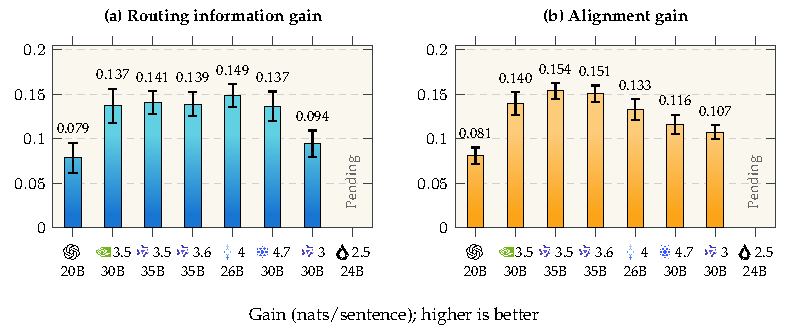
\includegraphics[width=\linewidth]{figures/journal/readout.pdf}
\caption{Routing information gain (RIG) over text in panel (a) and alignment gain over the lexical null in panel (b), in nats per sentence on a common scale.
%
Positive bars favor observed routing.
%
Horizontal labels give the mean gains.
%
Whiskers show the model-specific seven-comparison 95\% family-bootstrap intervals after reversing the loss-contrast sign.}
\label{fig:readout}
\end{figure}

The lexical-null comparison retains the same direction in every model.
%
Its original corrected gain intervals also exclude zero.
%
Thus the readout gain depends on information retained by the original routing alignment beyond the declared token and absolute-position stratification.
%
The baseline includes the current sentence and its available neighbours, so the gain reflects additional routing information.
%

This common direction supports reasoning-label information in sparse computation across several routing geometries.
%
The magnitude remains conditional on each model's generated text, available labels, and representation.
%
Comparing two gains is therefore not a controlled test of which architecture contains more interpretable reasoning.
%
The result establishes the increment within the specified prediction task.
%

\subsection{State balancing exposes a coverage trade-off}
\label{sec:selection-results}

State-balanced retention achieves higher weakest-state coverage (WSC) than labelled frequency in GPT-OSS, Nemotron, Gemma, GLM, Qwen3-30B, and LFM2.5 (Table~\ref{tab:selection}).
%
The direction holds in all five folds for each of these models.
%
Nemotron has the largest mean coverage gain, $\Delta\mathrm{WSC}=4.58$ percentage points, improving minimum coverage from 78.63\% to 83.22\%.
%
LFM2.5 improves by 3.46 points, GLM by 2.79 points, and GPT-OSS by 1.77 points.
%
These results show that the least-covered reasoning class can benefit from giving classes equal weight during expert selection.
%

% Adapted from SPSD tab:main-results and SYNCO tab:mainRes.
\begin{table}[tb]
\centering\small
\caption{Weakest-state coverage (WSC): the mean minimum held-out native selected-slot coverage across reasoning classes (\%) at 75\% expert retention.
%
Entries average the five family folds.
%
$\Delta\mathrm{WSC}$ is balanced minus frequency in percentage points.
%
Bold and underline mark the highest and second-highest selector means within each model.
%
The subscript n/e means that a 95\% confidence interval was not estimated in the saved outputs.
%
Individual values appear in Table~\ref{tab:selection-folds}.}
\label{tab:selection}
\setlength{\tabcolsep}{2.5pt}
\begin{adjustbox}{max width=\linewidth}
\begin{tabular}{@{}lrrrr@{}}
\toprule
 & \multicolumn{3}{c}{WSC (\%) $\uparrow$} & $\Delta\mathrm{WSC}$ (pp) \\
\cmidrule(lr){2-4}
Model & Balanced & Frequency & Random & Balanced $-$ frequency \\
\midrule
\modelname{openai}{GPT-OSS-20B} & $\mathbf{96.78}_{\mathrm{n/e}}$ & $\underline{95.01}_{\mathrm{n/e}}$ & $77.14_{\mathrm{n/e}}$ & $+1.77_{\mathrm{n/e}}$ \\ 
\modelname{nvidia}{\shortstack[l]{Nemotron-3.5-Lightning\\30B-A3B}} & $\mathbf{83.22}_{\mathrm{n/e}}$ & $\underline{78.63}_{\mathrm{n/e}}$ & $75.32_{\mathrm{n/e}}$ & $+4.58_{\mathrm{n/e}}$ \\ 
\modelname{qwen}{Qwen3.5-35B-A3B} & $\underline{91.62}_{\mathrm{n/e}}$ & $\mathbf{92.96}_{\mathrm{n/e}}$ & $75.09_{\mathrm{n/e}}$ & $-1.35_{\mathrm{n/e}}$ \\ 
\modelname{qwen}{Qwen3.6-35B-A3B} & $\underline{93.23}_{\mathrm{n/e}}$ & $\mathbf{93.78}_{\mathrm{n/e}}$ & $74.89_{\mathrm{n/e}}$ & $-0.55_{\mathrm{n/e}}$ \\ 
\modelname{gemma}{Gemma-4-26B-A4B} & $\mathbf{99.42}_{\mathrm{n/e}}$ & $\underline{99.20}_{\mathrm{n/e}}$ & $74.53_{\mathrm{n/e}}$ & $+0.21_{\mathrm{n/e}}$ \\ 
\modelname{zhipu}{GLM-4.7-Flash (30B-A3B)} & $\mathbf{89.28}_{\mathrm{n/e}}$ & $\underline{86.49}_{\mathrm{n/e}}$ & $74.04_{\mathrm{n/e}}$ & $+2.79_{\mathrm{n/e}}$ \\ 
\modelname{qwen}{Qwen3-30B-A3B} & $\mathbf{98.79}_{\mathrm{n/e}}$ & $\underline{98.21}_{\mathrm{n/e}}$ & $73.38_{\mathrm{n/e}}$ & $+0.59_{\mathrm{n/e}}$ \\ 
\modelname{liquid}{LFM2.5-24B-A2B} & $\mathbf{92.56}_{\mathrm{n/e}}$ & $\underline{89.10}_{\mathrm{n/e}}$ & $74.52_{\mathrm{n/e}}$ & $+3.46_{\mathrm{n/e}}$ \\ 
\bottomrule
\end{tabular}
\end{adjustbox}
\end{table}


Qwen3.5 and Qwen3.6 reverse this pattern.
%
Frequency has higher minimum coverage in every fold, by mean differences of 1.35 and 0.55 points, respectively.
%
This reversal occurs under the same training families, layer quotas, tie-breaking rule, and evaluation endpoint.
%
Equal class weight consequently does not supply a uniformly better allocation rule.
%
The coverage advantage of a selector depends on how class-specific allocation differs from the model's pooled labelled frequency.
%

\begin{figure}[tb]
\centering
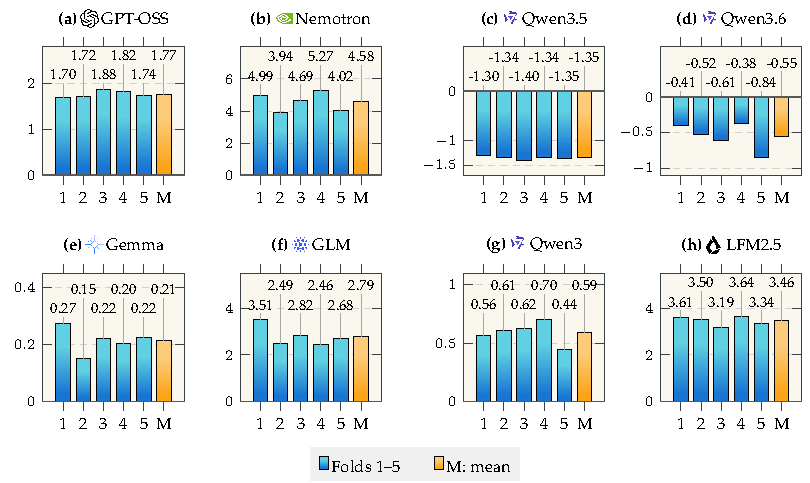
\includegraphics[width=\linewidth]{figures/journal/selection.pdf}
\caption{Gain in weakest-state coverage (WSC) at 75\% expert retention.
%
Positive values favor state balancing over labelled frequency.
%
Each model panel shows five fold-specific differences and their mean (M) in percentage points (pp), with model-specific vertical scales.}
\label{fig:selection}
\end{figure}

Gemma and Qwen3-30B retain 99.42\% and 98.79\% minimum class coverage under balancing.
%
Their mean gains over frequency are only 0.21 and 0.59 points, consistent with little remaining room for coverage improvement at this budget.
%
Nemotron retains a substantially smaller fraction under either learned selector, even though its balancing gain is larger.
%
Near-complete coverage indicates concentrated native allocation.
%
The paired difference measures the effect of changing the selection rule.
%

The fixed random masks have minimum coverage between 73.4\% and 77.2\% across model--fold cells.
%
Both learned methods improve on these masks in the reported mean comparison.
%
Their random baseline conditions on one set of priorities per model.
%
It does not estimate variation over independently sampled random masks.
%
All 120 model--fold--method cells are retained in Appendix~\ref{app:selection}.
%
The five folds partition test families, but their training sets overlap, so their spread supplies a stability description rather than five independent replications.
%

\subsection{Observed reasoning concentrates on analysis and implementation}
\label{sec:dynamics-results}

Implementation and analysis occupy most of the observed labelled tokens in every evaluated model (Figure~\ref{fig:occupancy}).
%
Implementation ranges from 31.18\% in GLM to 45.28\% in Gemma.
%
Analysis ranges from 24.38\% in Qwen3-30B to 31.76\% in Qwen3.5.
%
In contrast, monitoring occupies 2.79--8.17\% and verification 10.11--15.66\%.
%
These unequal shares explain why pooled labelled frequency and equal-class selection need not rank experts uniformly across reasoning activities.
%

\begin{figure}[tb]
\centering
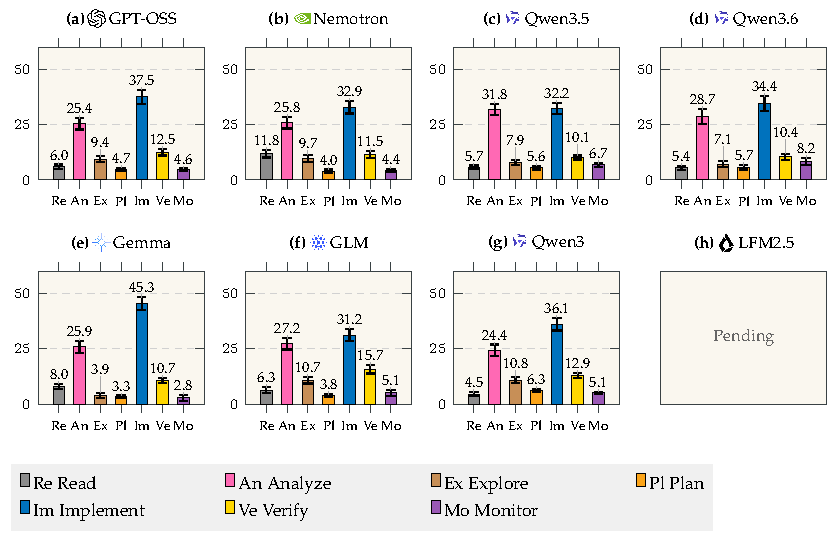
\includegraphics[width=\linewidth]{figures/journal/occupancy.pdf}
\caption{Seven reasoning-state occupancies among observed labelled tokens, shown in model panels on a common percentage scale.
%
Horizontal labels give means.
%
Whiskers show simultaneous 95\% confidence intervals within each model's native-dynamics panel, using 10,000 whole-family resamples.
%
Benchmarks and supported families receive equal weight.
%
Qwen3.6 uses 509 families.
%
The other evaluated models use 1,486.}
\label{fig:occupancy}
\end{figure}

The native summaries also quantify how much of the completion receives an observed label (Table~\ref{tab:label-coverage}).
%
Coverage ranges from 7.80\% for Qwen3.6 to 28.16\% for GPT-OSS under this equal-benchmark, equal-family estimand.
%
The occupancy comparison therefore describes the labelled part of the trace.
%
It cannot recover the classes of the remaining tokens or identify the complete temporal structure of a solution.
%
Qwen3.6 additionally has a smaller population in this analysis, so its distribution should be read with that support.
%


The complete seven-state distributions and their intervals appear in Appendix~\ref{app:dynamics}.
%
Variation in annotation coverage and the generated solutions is part of the comparison.
%
The displayed ordering of occupancy estimates supplies a descriptive pattern, while a claim about a difference between models would require a corresponding paired cross-model contrast.
%

\subsection{Verification entry differs from persistence}
\label{sec:transition-results}

The transition matrices expose how an observed activity connects to its next labelled sentence (Figure~\ref{fig:state-transitions}).
%
Implementation continues into another implementation sentence with mean probability \cid{48.61}{5.04}{5.04}\% in GPT-OSS and \cid{54.53}{6.70}{6.70}\% in Gemma.
%
The large implementation occupancy therefore accompanies substantial within-state persistence.
%
Moving from implementation to verification has mean probability \cid{17.27}{4.27}{4.27}\% in GPT-OSS and \cid{20.33}{4.81}{4.81}\% in Qwen3-30B (Table~\ref{tab:state-transitions}).
%
Repeating verification is more common than entering it from implementation in every evaluated model's point estimates.
%
This distinction separates access to a checking activity from persistence once it has started.
%
The overlapping model-specific intervals do not establish a cross-model ordering.
%

\begin{figure}[tb]
\centering
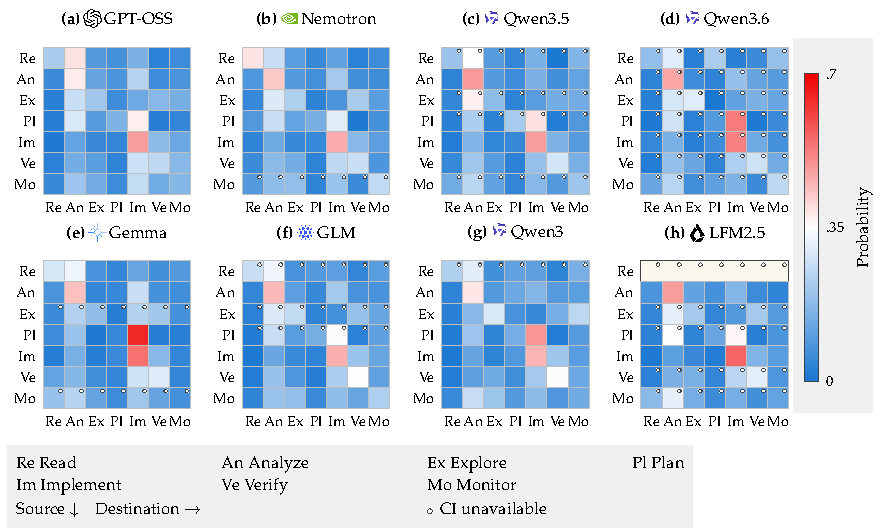
\includegraphics[width=\linewidth]{figures/journal/state_transitions.pdf}
\caption{Observed reasoning-state transitions in the eight evaluated models.
%
Rows denote the current state and columns the next adjacent labelled sentence.
%
Each row sums to one.
%
Colors encode saved equal-benchmark, equal-family mean probabilities on a common blue-to-red scale from 0 to 0.7.
%
Hollow corner marks identify cells whose original model-specific simultaneous 95\% whole-family-bootstrap interval is unavailable, including all Qwen3.6 transition cells and the sparsely supported LFM2.5 cells.
%
Missing-label gaps are not bridged.
%
Qwen3.6 uses 509 families.
%
Other evaluated models use 1,486.
%
Table~\ref{tab:state-transitions} gives selected means and confidence limits, and Appendix~\ref{app:dynamics} expands the duration comparison.}
\label{fig:state-transitions}
\end{figure}

% Native SYNCO tab:mainRes grouped diagnostic columns and caption-only key.
% Complete label-coverage and transition tables merged on identical model identity.
% Source: native_dynamics.json, unchanged saved means and interval endpoints.
\begin{table}[tb]
\centering\small
\caption{Annotation coverage and native state dynamics, with whole-family-bootstrap, model-specific simultaneous 95\% confidence intervals as subscripts.
%
Coverage is the labelled fraction of completion tokens.
%
Transition probabilities condition on the current state and next observed sentence boundary.
%
Missing-label gaps are not bridged.
%
Benchmarks and supported families receive equal weight.
%
Verify dwell includes contiguous labelled runs censored by coverage boundaries.
%
Qwen3.6's three transition intervals and LFM2.5's Verify persistence interval are unavailable under the saved support gate.
%
\textrm{An}, \textrm{Im}, and \textrm{Ve} denote Analyze, Implement, and Verify; n/e marks an unestimated interval.}
\label{tab:state-transitions}\label{tab:label-coverage}
\setlength{\tabcolsep}{2.5pt}
\begin{adjustbox}{max width=\linewidth}
\begin{tabular}{@{}lrccccc@{}}
\toprule
 & \multicolumn{2}{c}{Annotation} & \multicolumn{3}{c}{Transitions (\%)} & Dwell \\
\cmidrule(lr){2-3}\cmidrule(lr){4-6}\cmidrule(lr){7-7}
Model & Families & Coverage (\%) & \textrm{An} $\to$ \textrm{Im} & \textrm{Im} $\to$ \textrm{Ve} & \textrm{Ve} $\to$ \textrm{Ve} & \textrm{Ve} (tokens) \\
\midrule
\modelname{openai}{GPT-OSS-20B} & 1,486 & \cid{28.16}{0.93}{0.93} & \cid{24.17}{6.03}{6.03} & \cid{17.27}{4.27}{4.27} & \cid{25.29}{6.17}{6.17} & \cid{16.18}{1.06}{1.06} \\
\modelname{nvidia}{\shortstack[l]{Nemotron-3.5-Lightning\\30B-A3B}} & 1,486 & \cid{20.83}{1.17}{1.17} & \cid{21.31}{6.37}{6.37} & \cid{16.90}{4.93}{4.93} & \cid{26.73}{7.90}{7.90} & \cid{21.05}{1.96}{1.96} \\
\modelname{qwen}{Qwen3.5-35B-A3B} & 1,486 & \cid{8.06}{0.26}{0.26} & \cid{14.79}{5.22}{5.22} & \cid{15.43}{5.96}{5.96} & \cid{28.43}{9.90}{9.90} & \cid{14.35}{1.24}{1.24} \\
\modelname{qwen}{Qwen3.6-35B-A3B} & 509 & \cid{7.80}{0.39}{0.39} & $18.78_{\mathrm{n/e}}$ & $13.32_{\mathrm{n/e}}$ & $27.63_{\mathrm{n/e}}$ & \cid{13.67}{1.49}{1.49} \\
\modelname{gemma}{Gemma-4-26B-A4B} & 1,486 & \cid{16.27}{0.58}{0.58} & \cid{26.56}{6.57}{6.57} & \cid{16.89}{4.10}{4.10} & \cid{29.86}{8.36}{8.36} & \cid{17.95}{1.33}{1.33} \\
\modelname{zhipu}{GLM-4.7-Flash (30B-A3B)} & 1,486 & \cid{16.79}{1.22}{1.22} & \cid{21.13}{6.58}{6.58} & \cid{19.92}{6.71}{6.71} & \cid{34.54}{8.76}{8.76} & \cid{21.12}{1.33}{1.33} \\
\modelname{qwen}{Qwen3-30B-A3B} & 1,486 & \cid{15.90}{0.80}{0.80} & \cid{16.28}{4.73}{4.73} & \cid{20.33}{4.81}{4.81} & \cid{34.26}{6.83}{6.83} & \cid{16.53}{1.69}{1.69} \\
\modelname{liquid}{LFM2.5-24B-A2B} & 1,486 & \cid{9.96}{0.82}{0.82} & \cid{16.21}{7.70}{7.70} & \cid{15.83}{6.37}{6.37} & $30.61_{\mathrm{n/e}}$ & \cid{16.39}{2.04}{2.04} \\
\bottomrule
\end{tabular}
\end{adjustbox}
\end{table}


Observed verification runs also differ in duration.
%
Their mean token length is \cid{21.12}{1.33}{1.33} in GLM and \cid{13.67}{1.49}{1.49} in Qwen3.6.
%
Longer dwell can represent a sustained check, repeated checking, or a boundary introduced by sparse annotation.
%
It does not by itself identify wasted computation.
%
Routing guidance must therefore consider the candidate being checked and the usefulness of its continuation, alongside the state sequence.
%
These summaries describe the annotated segments, rather than a complete uncensored reasoning process.
%

\subsection{Routing anticipates the next reasoning state}
\label{sec:next-results}

The prospective comparison finds additional next-state information in GPT-OSS and Qwen3.6 (Figure~\ref{fig:next-state}).
%
The mean anticipatory routing gains (ARG) are \cid{0.02073}{0.00472}{0.00475} nats per pair for GPT-OSS and \cid{0.05570}{0.01417}{0.01374} for Qwen3.6.
%
The respective adjacent-pair populations contain 509 and 494 questions.
%

\begin{figure}[tb]
\centering
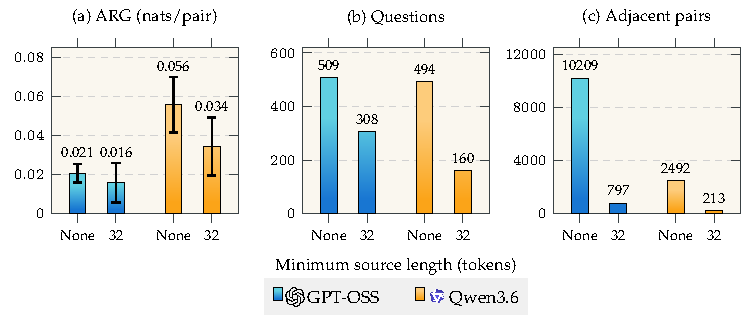
\includegraphics[width=.98\linewidth]{figures/journal/next_state.pdf}
\caption{Anticipatory routing gain and evaluation support under source-length restriction.
%
(a) ARG from trailing 16-token routing features; (b) contributing questions; (c) adjacent pairs.
%
None imposes no minimum source length; 32 requires at least 32 source tokens.
%
Positive ARG favors routing beyond past text and history.
%
Whiskers show the model-specific six-comparison 95\% family-bootstrap intervals.
%
Both conditions use source-owned tokens.
%
Equivalent estimates are unavailable for the other six listed models.}
\label{fig:next-state}
\end{figure}

Restricting eligible source sentences to at least 32 tokens preserves the positive direction in both models (Appendix~\ref{app:next-state}).
%
This restriction leaves 797 pairs from 308 questions in GPT-OSS and 213 pairs from 160 questions in Qwen3.6.
%
This sensitivity changes source-length support while retaining the same source-owned routing representation.
%

These gains support anticipation of the next assigned class from information available before its sentence.
%
They do not establish when a useful intervention should fire within that sentence.
%
Next-state estimates are unavailable for the other six models.
%

\subsection{Pulsed expert edits leave the reasoning state unchanged}
\label{sec:routing-results}

Targeted activation and deactivation do not move the observed reasoning state relative to matched random edits (Table~\ref{tab:routing}).
%
Across all models, targeted activation changes target-state occupancy by \cid{-0.11}{0.29}{0.29} percentage points (pp), and targeted deactivation by \cid{0.09}{0.31}{0.31} pp in the intended direction.
%
The first complete sentence after the prefix shows the same pattern, at \cid{-0.17}{0.35}{0.35} pp after activation and \cid{0.03}{0.51}{0.51} pp after deactivation.
%
These pooled intervals exclude state effects larger than about half a percentage point.
%
All 32 model-specific state contrasts contain zero, and their means range from $-0.79$ to $1.19$ pp without a common sign.
%

% Source: report/final-routing-20261015-r1/driver/analysis-final/EFFECTS.json via scripts/paper/export_routing_results.py.
\begin{table}[tb]
\centering\small
\caption{Paired effects of routing interventions at central strength, with family-bootstrap simultaneous 95\% confidence intervals as subscripts.
%
State columns give targeted minus matched-random arms in percentage points for target-state occupancy over the analysis window and for the first complete sentence; positive values favor the intended direction of activation or deactivation.
%
Efficiency columns compare targeted activation with matched random activation and with native routing, as accuracy in percentage points and generated tokens to the final answer in percent.
%
Each model uses its prepared family prefixes, 129 families except Nemotron and Qwen3-30B (128) and LFM2.5 (112).
%
Intervals are simultaneous over the four state contrasts or over all efficiency contrasts of the row.}
\label{tab:routing}
\setlength{\tabcolsep}{2.5pt}
\begin{adjustbox}{max width=\linewidth}
\begin{tabular}{@{}lcccccccc@{}}
\toprule
 & \multicolumn{4}{c}{Target state, targeted $-$ random (pp)} & \multicolumn{2}{c}{Activation $-$ random} & \multicolumn{2}{c}{Activation $-$ native} \\
\cmidrule(lr){2-5}\cmidrule(lr){6-7}\cmidrule(lr){8-9}
Model & Occ.\ act. & Occ.\ deact. & First act. & First deact. & Acc.\ (pp) & Tokens (\%) & Acc.\ (pp) & Tokens (\%) \\
\midrule
\modelname{openai}{GPT-OSS-20B} & \cid{-0.30}{1.07}{1.07} & \cid{-0.06}{0.78}{0.78} & \cid{-0.28}{1.22}{1.22} & \cid{-0.56}{1.36}{1.36} & \cid{-0.56}{3.01}{3.01} & \cid{0.0}{5.3}{5.3} & \cid{-0.87}{6.00}{6.00} & \cid{-0.4}{10.8}{10.8} \\
\modelname{nvidia}{Nemotron-3.5-Lightning-30B-A3B} & \cid{-0.38}{0.85}{0.85} & \cid{-0.15}{0.95}{0.95} & \cid{-0.06}{1.42}{1.42} & \cid{0.67}{1.40}{1.40} & \cid{1.06}{1.79}{1.79} & \cid{-2.1}{4.4}{4.4} & \cid{-0.21}{2.15}{2.15} & \cid{-7.5}{11.4}{11.4} \\
\modelname{qwen}{Qwen3.5-35B-A3B} & \cid{0.14}{0.90}{0.90} & \cid{-0.16}{0.94}{0.94} & \cid{0.20}{0.99}{0.99} & \cid{-0.20}{0.84}{0.84} & \cid{-0.24}{1.25}{1.25} & \cid{0.2}{5.8}{5.8} & \cid{-0.56}{1.49}{1.49} & \cid{-1.0}{9.2}{9.2} \\
\modelname{qwen}{Qwen3.6-35B-A3B} & \cid{-0.32}{0.64}{0.64} & \cid{0.12}{0.78}{0.78} & \cid{0.40}{0.66}{0.66} & \cid{-0.12}{0.97}{0.97} & \cid{-0.60}{1.74}{1.74} & \cid{-1.0}{4.3}{4.3} & \cid{-1.71}{4.56}{4.56} & \cid{-5.4}{9.1}{9.1} \\
\modelname{gemma}{Gemma-4-26B-A4B} & \cid{0.21}{0.67}{0.67} & \cid{0.20}{0.81}{0.81} & \cid{-0.12}{0.75}{0.75} & \cid{0.16}{0.97}{0.97} & \cid{1.03}{2.34}{2.34} & \cid{2.1}{6.3}{6.3} & \cid{-0.95}{1.53}{1.53} & \cid{-3.9}{9.8}{9.8} \\
\modelname{zhipu}{GLM-4.7-Flash (30B-A3B)} & \cid{-0.57}{0.96}{0.96} & \cid{0.45}{1.18}{1.18} & \cid{-0.79}{1.61}{1.61} & \cid{1.19}{1.44}{1.44} & \cid{-0.12}{3.18}{3.18} & \cid{0.0}{5.9}{5.9} & \cid{-0.36}{5.90}{5.90} & \cid{-2.4}{12.9}{12.9} \\
\modelname{qwen}{Qwen3-30B-A3B} & \cid{0.48}{0.85}{0.85} & \cid{0.31}{0.75}{0.75} & \cid{-0.24}{0.88}{0.88} & \cid{-0.75}{2.02}{2.02} & \cid{0.62}{3.52}{3.52} & \cid{0.1}{4.6}{4.6} & \cid{-1.16}{3.96}{3.96} & \cid{2.8}{8.9}{8.9} \\
\modelname{liquid}{LFM2.5-24B-A2B} & \cid{-0.09}{0.74}{0.74} & \cid{0.07}{0.88}{0.88} & \cid{-0.55}{1.26}{1.26} & \cid{-0.20}{1.07}{1.07} & \cid{0.44}{2.38}{2.38} & \cid{-4.8}{8.5}{8.5} & \cid{-1.07}{4.93}{4.93} & \cid{-0.5}{13.4}{13.4} \\
\midrule
All models & \cid{-0.11}{0.29}{0.29} & \cid{0.09}{0.31}{0.31} & \cid{-0.17}{0.35}{0.35} & \cid{0.03}{0.51}{0.51} & \cid{0.20}{0.87}{0.87} & \cid{-0.7}{2.1}{2.1} & \cid{-0.89}{1.60}{1.60} & \cid{-2.4}{3.8}{3.8} \\
\bottomrule
\end{tabular}
\end{adjustbox}
\end{table}


The absent state response does not reflect an inactive edit.
%
The engineering gate confirmed that activation placed and deactivation removed the nominated experts at every pulse token, while a zero-length pulse reproduced native generation exactly.
%
Every production run also verified the native routing equation at each hooked layer.
%
The analysis retains all 29,377 assigned continuations, including those that reach their original generation allowance.
%
The lexical readout of the generated sentences does not limit this conclusion: dividing each class-specific activation effect by the readout's native Youden index leaves every corrected 95\% interval containing zero (Appendix~\ref{app:lexical-readout}).
%

\begin{figure}[tb]
\centering
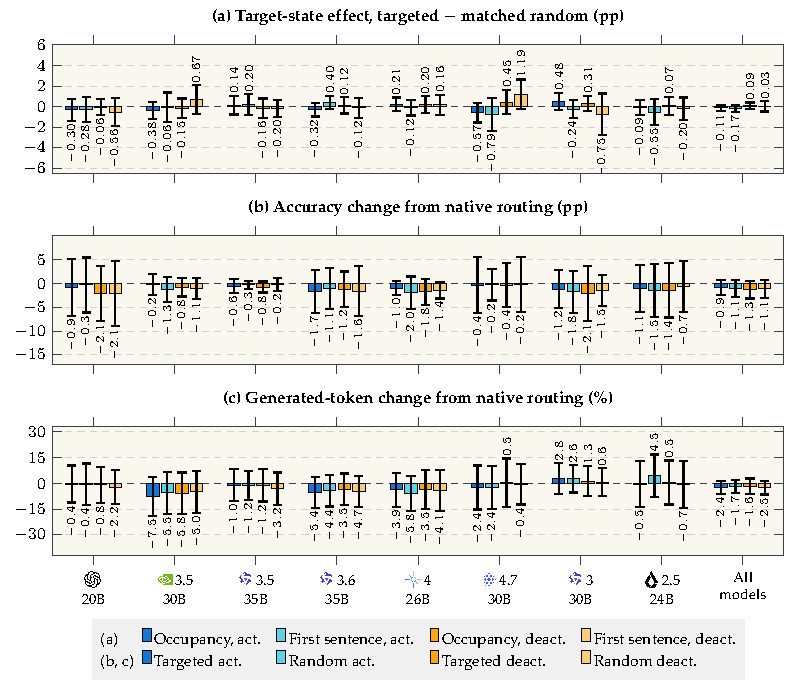
\includegraphics[width=\linewidth]{figures/journal/routing.pdf}
\caption{Paired effects of routing interventions at central strength.
%
(a) Target-state occupancy and first-sentence state for targeted minus matched random edits, signed so that positive values favor the intended direction.
%
(b) Accuracy and (c) generated tokens to the final answer for each edited arm relative to native routing.
%
Labels give the means, and whiskers show family-bootstrap simultaneous 95\% confidence intervals within each model and contrast family.
%
The pooled group averages models and classes within each family before weighting benchmarks equally.}
\label{fig:routing}
\end{figure}

The edits also leave generation cost and answer quality unchanged.
%
Relative to matched random activation, targeted activation changes accuracy by \cid{0.20}{0.87}{0.87} pp and generated tokens by \cid{-0.7}{2.1}{2.1}\%.
%
Relative to native routing, every edited arm has a lower mean accuracy, by 0.89 to 1.31 pp, and 1.6 to 2.5\% fewer generated tokens (Figure~\ref{fig:routing}).
%
Each of these intervals contains zero under the simultaneous correction across the efficiency contrasts.
%
Without that correction, the 1.31-point loss after targeted deactivation has a 95\% interval from $-2.49$ to $-0.13$ pp, so a small accuracy cost of editing cannot be excluded.
%
Appendix~\ref{app:routing-levels} reports the accuracy and token levels of every arm.
%

Native traces nevertheless associate reasoning states with the remaining solution length.
%
At the same question and absolute position, a Verify or Monitor sentence precedes shorter remaining reasoning in all seven models with saved native labels, whereas an Analyze sentence precedes longer remaining reasoning in all seven (Appendix~\ref{app:efficiency-link}).
%
Before any intervention outcome existed, we pre-registered the prediction that the token effect of each model--class edit would follow the sign and rank of this native association.
%
The measured token effects do not follow it: their Spearman correlation with the native associations across 49 model--class cells is $-0.11$, with a 95\% interval from $-0.29$ to $0.13$, and the signs agree in 41\% of the 41 signed cells.
%
The corresponding accuracy correlation is $0.07$, from $-0.16$ to $0.31$.
%
A state that accompanies shorter native solutions therefore does not shorten generation when its nominated experts are activated.
%

A stronger exploratory edit leaves the same conclusion.
%
Forcing the high-count nominated sets at all three depth regions throughout the analysis window changes target-state occupancy by \cid{0.04}{0.46}{0.46} pp relative to the matched forced controls in four models (Appendix~\ref{app:routing-strong}).
%
Both forced arms lower mean accuracy relative to native routing, by \cid{1.52}{2.18}{2.18} pp for the nominated sets and \cid{1.35}{2.37}{2.37} pp for the controls.
%
We specified this arm after inspecting the primary contrasts, so it qualifies the central result without replacing it.
%

\subsection{Sustained steering changes the computation, not the reasoning state}
\label{sec:whole-results}

Steering the efficiency-directed states throughout the reasoning makes no model reason more efficiently than matched random edits (Table~\ref{tab:whole}).
%
At full strength, the targeted composite lengthens the reasoning of GPT-OSS-20B by \cid{40.9}{31.8}{31.8}\% and lowers the accuracy of Nemotron by \cid{-10.43}{6.56}{6.56} pp and of Qwen3-30B by \cid{-14.28}{14.10}{14.10} pp, and the intervals of the other models contain zero.
%
Across all models, the composite changes reasoning tokens by \cid{-9.9}{375.6}{375.6}\% and accuracy by \cid{-8.87}{15.67}{15.67} pp, so no model meets the efficiency criterion of Section~\ref{sec:whole-steering}.
%
Relative to native routing, mean accuracy falls by 14.34 pp after targeted edits and by 5.47 pp after matched random edits.
%

The composite averages states whose effects differ in direction and size (Figure~\ref{fig:whole-states}).
%
At base strength, 8.0\% of the targeted-minus-random contrasts have simultaneous intervals that exclude zero, and each of them lengthens the reasoning or lowers accuracy.
%
Suppressing Implement lowers accuracy by \cid{-48.59}{24.96}{24.96} pp in Nemotron and by \cid{-42.88}{21.19}{21.19} pp in Qwen3-30B.
%
Suppressing Analyze lowers accuracy by \cid{-26.81}{19.89}{19.89} pp in Qwen3.6 and by \cid{-15.23}{10.92}{10.92} pp in Nemotron, whose reasoning it also lengthens by \cid{80.2}{52.8}{52.8}\%.
%
In GPT-OSS-20B at half strength, promoting Read, Analyze, Explore or Plan multiplies the reasoning length by 3.8 to 6.2 and lowers accuracy by 45.6 to 60.6 pp, in the direction of the native association of these states with longer remaining reasoning (Appendix~\ref{app:efficiency-link}).
%

The edits change the computation more than the reasoning state.
%
Against matched random edits, the occupancy of the steered state changes by a median of $-0.03$ pp of the generation allowance, and the intervals of 4.6\% of the steered cells exclude zero (Table~\ref{tab:whole-occupancy}).
%
Promoting Explore and Plan in GPT-OSS-20B raises their occupancy by 1.93 and 0.75 pp, whereas suppressing Implement in Nemotron raises the occupancy of Implement itself by 36.72 pp of the allowance.
%

Varying the number of edited pairs reveals no efficient strength (Figure~\ref{fig:whole-dose}).
%
Across all models, the composite changes reasoning tokens by \cid{-12.7}{172.3}{172.3}\%, \cid{-9.5}{250.9}{250.9}\% and \cid{-9.9}{392.9}{392.9}\% at quarter, half and full strength, while the mean accuracy change falls from $-3.40$ pp to $-6.70$ pp and $-8.87$ pp at the same strengths.
%
The pooled slope of Equation~\eqref{eq:whole-slope} is \cid{-2.73}{12.55}{12.55} accuracy points per doubling of the edited pairs, and its token slope is centered on zero.
%
Breakdown remains rare and concentrates in two models.
%
No native continuation reaches the length limit, while the share of targeted continuations that reach it rises from 0.7\% at quarter strength to 5.7\% at full strength in Nemotron and lies between 8.9\% and 10.6\% in Qwen3-30B, against at most 0.8\% in the other models.
%

% Source: report/whole-reasoning-20261021-r14/analysis-combined/EFFECTS_WHOLE.json via scripts/paper/export_whole_results.py.
\begin{table}[tb]
\centering\small
\caption{Paired effects of routing edits at full strength on reasoning tokens and strict accuracy, with family-bootstrap simultaneous 95\% confidence intervals as subscripts.
%
Targeted edits promote or suppress the efficiency-directed states of each model, random edits use matched control expert sets, and native routing is unedited; each column pair compares the first arm with the second.
%
Tokens give the percent change in reasoning tokens, with negative values meaning fewer tokens, and accuracy differences are in percentage points.
%
Intervals are simultaneous over the rows and both outcomes of each comparison and cover the outcome bounds of unfinished continuations.
%
GPT-OSS-20B and GLM-4.7-Flash ran full strength in the strength sweep.}
\label{tab:whole}
\setlength{\tabcolsep}{2.5pt}
\begin{adjustbox}{max width=\linewidth}
\begin{tabular}{@{}lcccccc@{}}
\toprule
 & \multicolumn{2}{c}{Targeted $-$ random} & \multicolumn{2}{c}{Targeted $-$ native} & \multicolumn{2}{c}{Random $-$ native} \\
\cmidrule(lr){2-3}\cmidrule(lr){4-5}\cmidrule(lr){6-7}
Model & Tokens (\%) & Acc.\ (pp) & Tokens (\%) & Acc.\ (pp) & Tokens (\%) & Acc.\ (pp) \\
\midrule
\modelname{openai}{GPT-OSS-20B} & \cid{40.9}{31.8}{31.8} & \cid{-5.81}{6.29}{6.29} & \cid{160.8}{550.3}{550.3} & \cid{-12.94}{14.15}{14.15} & \cid{85.1}{374.9}{374.9} & \cid{-7.13}{15.52}{15.52} \\
\modelname{nvidia}{Nemotron-3.5-Lightning-30B-A3B} & \cid{21.2}{59.3}{59.3} & \cid{-10.43}{6.56}{6.56} & \cid{39.7}{78.0}{78.0} & \cid{-17.07}{8.72}{8.72} & \cid{15.3}{13.4}{13.4} & \cid{-6.64}{5.89}{5.89} \\
\modelname{qwen}{Qwen3.5-35B-A3B} & \cid{20.6}{3414.3}{3414.3} & \cid{-2.19}{29.91}{29.91} & \cid{-15.0}{1521.9}{1521.9} & \cid{-7.42}{27.16}{27.16} & \cid{-29.5}{1570.7}{1570.7} & \cid{-5.22}{28.34}{28.34} \\
\modelname{qwen}{Qwen3.6-35B-A3B} & \cid{-45.8}{240.0}{240.0} & \cid{-13.69}{16.61}{16.61} & \cid{-52.1}{196.5}{196.5} & \cid{-15.69}{16.64}{16.64} & \cid{-11.6}{77.3}{77.3} & \cid{-2.00}{7.19}{7.19} \\
\modelname{gemma}{Gemma-4-26B-A4B} & \cid{-23.2}{809.1}{809.1} & \cid{-4.70}{23.61}{23.61} & \cid{-20.3}{510.0}{510.0} & \cid{-11.35}{19.29}{19.29} & \cid{3.8}{486.2}{486.2} & \cid{-6.65}{16.35}{16.35} \\
\modelname{zhipu}{GLM-4.7-Flash (30B-A3B)} & \cid{-32.3}{1573.1}{1573.1} & \cid{-13.06}{29.49}{29.49} & \cid{-11.8}{2580.1}{2580.1} & \cid{-15.94}{30.47}{30.47} & \cid{30.3}{1047.4}{1047.4} & \cid{-2.89}{19.45}{19.45} \\
\modelname{qwen}{Qwen3-30B-A3B} & \cid{7.5}{262.7}{262.7} & \cid{-14.28}{14.10}{14.10} & \cid{16.3}{295.3}{295.3} & \cid{-20.88}{16.50}{16.50} & \cid{8.2}{264.1}{264.1} & \cid{-6.60}{14.78}{14.78} \\
\modelname{liquid}{LFM2.5-24B-A2B} & \cid{-31.2}{1218.8}{1218.8} & \cid{-6.61}{28.17}{28.17} & \cid{-34.2}{547.3}{547.3} & \cid{-13.20}{23.29}{23.29} & \cid{-4.3}{258.3}{258.3} & \cid{-6.59}{15.53}{15.53} \\
\midrule
All models & \cid{-9.9}{375.6}{375.6} & \cid{-8.87}{15.67}{15.67} & \cid{-2.4}{343.7}{343.7} & \cid{-14.34}{15.08}{15.08} & \cid{8.3}{213.5}{213.5} & \cid{-5.47}{10.88}{10.88} \\
\bottomrule
\end{tabular}
\end{adjustbox}
\end{table}


\begin{figure}[tb]
\centering
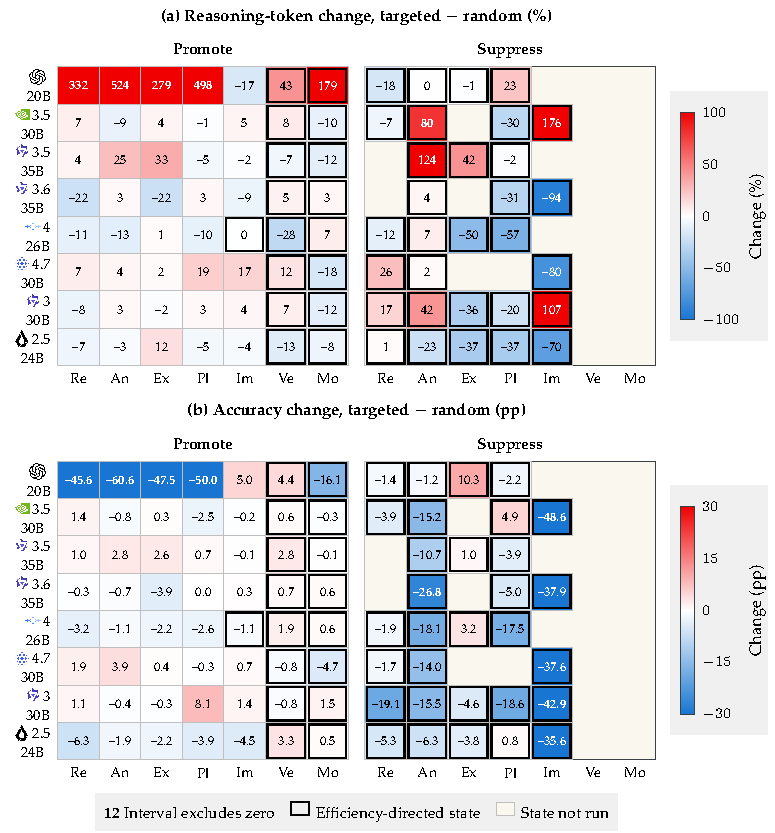
\includegraphics[width=\linewidth]{figures/journal/whole_states.pdf}
\caption{Per-state effects of steering the whole reasoning at each model's base strength, targeted against matched random edits.
%
Panel (a) gives the percent change in reasoning tokens, with negative values meaning fewer tokens, and panel (b) gives the change in strict accuracy in percentage points.
%
Rows are models, and in each panel the left block promotes a state while the right block suppresses it.
%
Re, An, Ex, Pl, Im, Ve and Mo abbreviate Read, Analyze, Explore, Plan, Implement, Verify and Monitor.
%
Blue marks a decrease and red an increase, with the color scale clipped at $\pm$100\% in (a) and $\pm$30 pp in (b), while printed values are not clipped.
%
Bold numbers have a family-bootstrap simultaneous 95\% interval, over the outcome bounds of unfinished continuations, that excludes zero.
%
Outlined cells are efficiency-directed states, and empty cells are states the model does not suppress.
%
The base strength is full except for GPT-OSS-20B and GLM-4.7-Flash, which use half strength.}
\label{fig:whole-states}
\end{figure}

\begin{figure}[tb]
\centering
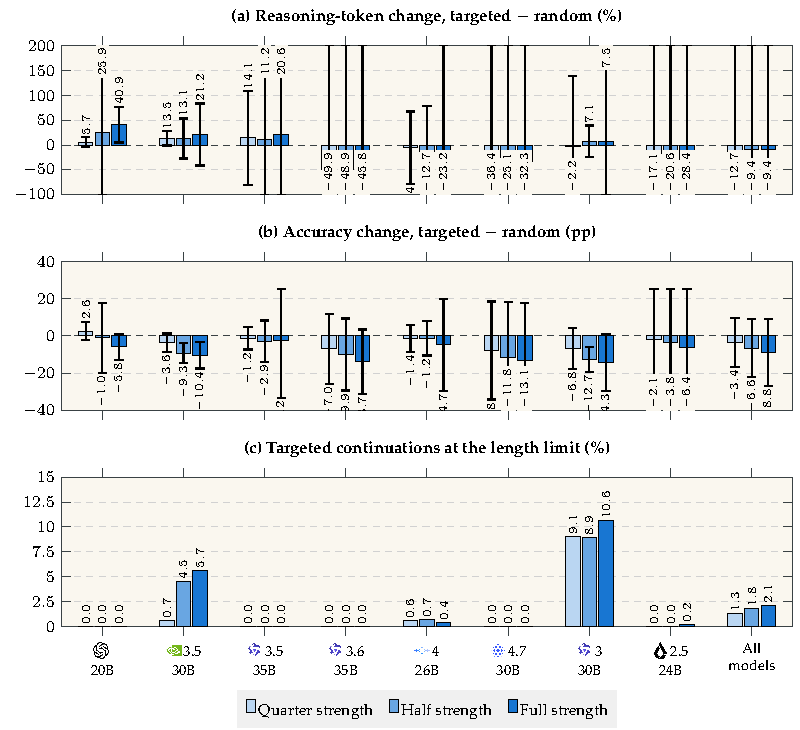
\includegraphics[width=\linewidth]{figures/journal/whole_dose.pdf}
\caption{Efficiency of steering the whole reasoning at quarter, half and full strength.
%
Panels (a) and (b) give the reasoning-token and accuracy change of targeted against matched random edits, averaged over each model's efficiency-directed states, and panel (c) gives the share of targeted continuations of these states that reach the length limit.
%
Labels give the means, and whiskers show family-bootstrap simultaneous 95\% intervals over all strengths, models and outcome bounds, cut at the panel edge when they extend beyond it.
%
The pooled group averages the models within each family before weighting benchmarks equally.}
\label{fig:whole-dose}
\end{figure}

\subsection{Promotion changes engagement without establishing control}
\label{sec:utility-results}

Historical Qwen3.6 prefix interventions increase target inclusion relative to native routing (Appendix~\ref{app:interventions}).
%
The mean intended target-inclusion fraction increases by \cid{0.1376}{0.0613}{0.0506} when two targets are promoted across eight verification families.
%
Single-pulse promotion in a second pilot increases it by \cid{0.2940}{0.1663}{0.1821}, across thirteen families covering verification and commitment transitions.
%
These are routing-engagement outcomes.
%
The larger fresh comparison leaves the semantic effect uncertain under the original simultaneous intervals and missing-judgment bounds (Appendix~\ref{app:interventions}).
%
More target inclusion does not by itself establish substantive verification.
%

Complete historical global steering does not establish a positive accuracy effect and includes harmful policies (Appendix~\ref{app:interventions}).
%
The separate candidate-recognition protocol does not qualify in five evaluated models and remains incomplete in two (Appendix~\ref{app:verification-qualification}).
%
Together with the paired continuations, these results separate a change in the selected experts from a change in the reasoning the model produces.
%

\section{Discussion and Limitations}
\label{sec:discussion}

\subsection{Routing carries information beyond text}

The eight-model readout demonstrates information about assigned reasoning states beyond the declared text baseline.
%
Its lexical null tests the original alignment of route paths under token-identity and absolute-position controls.
%
The shared direction across models supports the use of routing as an additional measurement of visible reasoning.
%
The target remains an automatically assigned sentence label, and the result does not establish a latent cognitive module or a dedicated expert for that reasoning activity.
%

The retrospective baseline makes the supported claim particularly specific.
%
It observes the sentence being classified and the same neighbouring context as the annotation reader.
%
This controls for substantial text information, but it also means that the classifier is evaluated after the target text exists.
%
The two-model next-state analysis supplies separate prospective evidence.
%
Extending that claim to the other models requires their own temporally valid evaluation.
%

\subsection{Unequal state mass does not guarantee a coverage gain}

Class balancing changes how training allocations are weighted.
%
A common class contributes many selected slots to frequency, while the balanced criterion gives each supported class equal weight.
%
The observed occupancy distributions show substantial inequality in labelled token mass.
%
Such inequality makes the balancing comparison meaningful, but does not determine its result.
%
The useful experts for a rare class may already be retained by frequency, or a balanced ranking may displace experts that cover several classes together.
%

The five-fold reversal in Qwen3.5 and Qwen3.6 shows that this trade-off survives changes in which families are held out.
%
The positive effects in the other six models establish a different allocation pattern under the same budget.
%
Neither pattern selects a universal pruning rule.
%
Gemma and Qwen3-30B also show that a selector can have near-complete native coverage with a small difference between criteria.
%
A large coverage gain and a high absolute coverage answer different deployment questions.
%

The comparison is restricted to labelled-token frequency.
%
Conventional all-token frequency and output-aware criteria use additional information, and the random arm conditions on one fixed priority set per model.
%
Coverage is averaged across routed layers, so it can also hide a concentrated loss at a particular layer.
%
The per-layer and per-class records remain necessary when interpreting any proposed removal.
%

\subsection{Sparse labels bound the scientific claim}

The reader assigns labels to visible language.
%
Its external validation and prompt-selection tests do not establish perfect agreement on each model's generated mathematical text.
%
Labels are also sparse, and gaps prevent complete reconstruction of reasoning trajectories.
%
Reporting coverage alongside occupancy retains this limitation in the state-distribution analysis.
%

The independent problem unit is a duplicate family for the routing analyses and a response for the external SAT probes.
%
Sentences, tokens, and repeated branches remain dependent measurements within those units.
%
The original readout intervals condition on saved fits, and the retention comparison reports fold stability with overlapping training sets.
%
The native-dynamics intervals use their own model-specific simultaneous panels.
%
None of these summaries supplies variation over repeated model generations or a new simultaneous test across the complete collection of studies.
%

The analysis covers mathematical problem solving under the retained model and decoding profiles.
%
It does not establish transfer to other reasoning domains, other quantizations, or a changed route-selection implementation.
%
Expert identities and score semantics are local to the model.
%
Historical correlations with correctness (\mbox{Appendix~\ref{app:associations}}) also depend on problem difficulty, length, and termination.
%

\subsection{Routing records reasoning states without steering them}

The paired continuations separate two properties that the earlier evidence could not distinguish.
%
Routing carries information about the present and next reasoning state, and native states differ in how much reasoning remains after them.
%
Changing which experts compute a short pulse at a reasoning boundary nevertheless leaves the next state, the state occupancy over hundreds of tokens, and the generation cost within narrow intervals of the matched random edit.
%
Forcing the nominated sets at three depths throughout the analysis window does not change this result and lowers mean accuracy for both target and control sets.
%
The routes that accompany a reasoning activity therefore behave as a record of that activity rather than as a control that selects it.
%

Several properties of the design bound this conclusion.
%
Nomination ranks experts by their inclusion excess for a class, so the target sets may track lexical form or position rather than the computation that decides the next activity.
%
Each class and fold edits one layer at a fixed central count, and the remaining layers keep their native routes, which can compensate for a local change.
%
The lexical readout attenuates occupancy contrasts by its Youden index, yet the corrected intervals remain near zero.
%
The continuations start from frozen prefixes in the middle of solutions, so they do not estimate a policy applied from the first token.
%
A different nomination criterion, a multi-layer or adaptive edit, or a readout of hidden-state change might still reveal a controllable route.
%

The accuracy results also carry a practical caution.
%
Every edited arm has a lower mean accuracy than native routing, and the sustained strong edit lowers it by about one and a half points.
%
These losses lie within simultaneous intervals that include zero, so they do not establish harm, but they show that a routing edit is not free of cost.
%
A non-significant accuracy difference alone cannot establish that accuracy is retained.
%

\section{Conclusion}
\label{sec:conclusion}

Routing interventions alter the sparse computation performed by MoE LLMs while retaining their weights.
%
In mathematical problem solving, native routes carry information about visible reasoning states, and states such as verification precede shorter remaining reasoning.
%
The observed state transitions distinguish entry into verification from persistence within it.
%
State balancing changes which activities a limited expert set covers, with an advantage that depends on the model.
%
Activating or deactivating the experts nominated for a reasoning state, however, changes neither the following state nor the cost and accuracy of the solution beyond matched random edits.
%
Routing therefore reveals reasoning states more readily than it controls them.
%
Efficient reasoning through routing will require interventions that change the computation deciding the next activity rather than the experts that accompany it.
%

\paragraph{Data and code availability}
The analysis implementation, compact result tables, editable figure sources, and manuscript are maintained in the project repository.
%
Model revisions and the retained statistical estimates are documented in the supplementary material.
%
Model weights remain subject to their original licenses.
%
Bulk routing captures are not included in the manuscript source package.
%


\begin{acknowledgments}
Generative AI assistants were used for manuscript editing, inspection of saved experimental artifacts, and assistance with code and analysis development.
%
The authors are responsible for the paper's claims, citations, and interpretation of the results.
%
\end{acknowledgments}

\bibliographystyle{compling}
\bibliography{references}

% Structural boundary: appendix floats must not precede the bibliography.
\clearpage
\appendix
% CL resets appendix counters and uses starred headings. Give those objects
% unique PDF destinations while preserving its printed headings and numbering.
\makeatletter
\renewcommand*{\theHsection}{appendix.\Alph{section}}
\renewcommand*{\theHsubsection}{\theHsection.\arabic{subsection}}
\renewcommand*{\theHsubsubsection}{\theHsubsection.\arabic{subsubsection}}
\renewcommand*{\theHtable}{\theHsection.\arabic{table}}
\renewcommand*{\theHfigure}{\theHsection.\arabic{figure}}
\renewcommand*{\theHequation}{\theHsection.\arabic{equation}}
\renewcommand{\journalappendix}[2]{\appendixsection{#1}%
  \setcounter{subsection}{0}\setcounter{subsubsection}{0}%
  \phantomsection
  \protected@edef\@currentlabel{\Alph{section}}\label{#2}}
\makeatother

\renewcommand{\thesection}{\Alph{section}}
\journalappendix{Readout Estimates and Temporal Support}{app:readout}

Table~\ref{tab:readout-detail} supplies the complete present-state contrasts behind Figure~\ref{fig:readout}.
%
Sentence counts differ because each model generates its own solution and contributes its own labelled sentences.
%
The independent question and family population is common.
%
Positive RIG favors the routing-augmented classifier.
%

% Adapted from SPSD tab:main-results and SYNCO tab:mainRes.
\begin{table}[hb]
\centering\small
\caption{Routing information gain (RIG): text-baseline cross-entropy minus routing-augmented cross-entropy (nats per sentence), with 95\% confidence intervals as subscripts.
%
Each evaluated model uses 522 questions in 509 families.
%
Intervals retain the original model-specific seven-comparison family-bootstrap correction.
%
Bold and underline mark the largest and second-largest mean gains descriptively.
%
Dashes denote pending LFM2.5 results.}
\label{tab:readout-detail}
\setlength{\tabcolsep}{2.5pt}
\begin{adjustbox}{max width=\linewidth}
\begin{tabular}{@{}lrc@{}}
\toprule
Model & Sentences & RIG (nats) $\uparrow$ \\
\midrule
\modelname{openai}{GPT-OSS-20B} & 37,549 & \cid{0.07858}{0.01679}{0.01709} \\ 
\modelname{nvidia}{\shortstack[l]{Nemotron-3.5-Lightning\\30B-A3B}} & 35,334 & \cid{0.13721}{0.01902}{0.01907} \\ 
\modelname{qwen}{Qwen3.5-35B-A3B} & 34,740 & \secondcid{0.14090}{0.01309}{0.01269} \\ 
\modelname{qwen}{Qwen3.6-35B-A3B} & 35,484 & \cid{0.13899}{0.01297}{0.01378} \\ 
\modelname{gemma}{Gemma-4-26B-A4B} & 31,902 & \bestcid{0.14866}{0.01174}{0.01269} \\ 
\modelname{zhipu}{GLM-4.7-Flash (30B-A3B)} & 38,931 & \cid{0.13679}{0.01644}{0.01623} \\ 
\modelname{qwen}{Qwen3-30B-A3B} & 36,445 & \cid{0.09427}{0.01326}{0.01502} \\ 
\modelname{liquid}{LFM2.5-24B-A2B} & \textemdash & \textemdash \\
\bottomrule
\end{tabular}
\end{adjustbox}
\end{table}


\subsection{Readout representations and model selection}
\label{app:readout-features}

The readout tests information about the assigned sentence label while holding the evaluation families fixed.
%
Token-identity features use 4,096 buckets, retain terms supported by at least two training sentences, and apply sublinear term-frequency/inverse-document-frequency weighting.
%
Each resulting row is normalized to Euclidean length one and scaled by ten.
%
The extended reader-context representation hashes word unigrams and bigrams and character 3-, 4-, and 5-grams into $2^{18}$ buckets, with the same row scale.
%
Only training data determine the frequency weights.
%
Dense routing features are standardized within the training fold.
%
Coordinate means and population standard deviations use the training rows.
%
A nonfinite mean is replaced by zero, a standard deviation at most $10^{-12}$ by one, and a missing standardized value by zero.
%

Let $a_{\ell,t}$ be the top-1 expert at sparse layer $\ell$ for token $t$.
%
For each adjacent layer pair, training-token counts $N_\ell(a,b)$ define the smoothed conditional probability
\begin{equation}
\widehat p_\ell(b\mid a)=
\frac{N_\ell(a,b)+0.5}{\sum_{b'}N_\ell(a,b')+0.5E}.
\end{equation}
Here $E$ is the number of experts per sparse layer.
%
Depth-path surprise $D_s$ is the sentence mean of $-\log\widehat p_\ell(a_{\ell+1,t}\mid a_{\ell,t})$, averaged equally over its tokens and the $L-1$ adjacent layer pairs.
%
It measures how unexpected the observed sequence of expert identities across depth is under the training transitions.
%
It is nonnegative in nats and has no population-independent finite upper bound.
%

Temporal persistence measures the fraction of layers retaining the same top-1 expert between consecutive tokens.
%
For a sentence $j$, let $A_j$ contain its token positions whose preceding token is adjacent and belongs to that sentence.
%
The feature is
\begin{equation}
R_j=\frac{1}{|A_j|L}\sum_{t\in A_j}\sum_{\ell=1}^{L}
\mathbf{1}\{a_{\ell,t}=a_{\ell,t-1}\}.
\end{equation}
Its range is zero to one, where one means that every layer retains its top-1 identity across every supported token pair.
%
When $A_j$ is empty, the feature is missing and becomes zero after training-fold standardization, the standardized training mean.
%
Neither feature bridges a sentence boundary or a missing-token gap.
%

The routing composition is centered on the training mean and projected to 64 principal components.
%
The retained randomized decomposition uses 16 oversampling directions and four power iterations.
%
Routing features also contain depth-path surprise and temporal persistence.
%
Multinomial ridge fitting selects its penalty from $10^{-3},10^{-2},10^{-1},1,10,100$ by inner held-out cross-entropy, breaking ties toward stronger regularization.
%
The five outer and three inner folds keep duplicate families together.
%
All transforms are fitted anew on each training split.
%
The saved intervals condition on these fitted readouts.
%
The routing-augmented penalty is 0.01 in every outer fold for the seven original models and 0.001 for LFM2.5.
%
The text penalty is 0.001 throughout for GPT-OSS, Nemotron, Qwen3.5, Qwen3.6 and Qwen3-30B, and 0.01 throughout for Gemma.
%
GLM uses 0.001, 0.01, 0.01, 0.001 and 0.001 in fold order.
%

\subsection{Next-state support}
\label{app:next-state}
The original next-state endpoint and its source-length sensitivity have different question and pair counts (Table~\ref{tab:next-state}).
%
Both use only tokens owned by the source sentence.
%
The sensitivity retains sources with at least 32 tokens, ensuring a full 16-token trailing window.
%
It restricts eligible pairs without restricting the sentences used to build profiles within the selected training attempts.
%
Loss averages pairs within a question before averaging questions, and resampling keeps duplicate families together.
%

% Adapted from SPSD tab:main-results and SYNCO tab:mainRes.
\begin{table}[htb]
\centering\small
\caption{Anticipatory routing gain (ARG): past-text/history baseline cross-entropy minus routing-augmented cross-entropy (nats per adjacent pair), with 95\% confidence intervals as subscripts.
%
Intervals retain the original six-comparison family-bootstrap correction.
%
Bold and underline mark the larger and second-largest mean gains within each source-length condition.
%
The length column gives the minimum source-sentence length in tokens.
%
Both use source-owned tokens.}
\label{tab:next-state}
\setlength{\tabcolsep}{2.5pt}
\begin{adjustbox}{max width=\linewidth}
\begin{tabular}{@{}llrrc@{}}
\toprule
Model & Length & Questions & Pairs & ARG (nats) $\uparrow$ \\
\midrule
\modelname{openai}{GPT-OSS-20B} & None & 509 & 10,209 & \secondcid{0.02073}{0.00472}{0.00475} \\ 
\modelname{openai}{GPT-OSS-20B} & 32 & 308 & 797 & \secondcid{0.01570}{0.00923}{0.01005} \\ 
\modelname{qwen}{Qwen3.6-35B-A3B} & None & 494 & 2,492 & \bestcid{0.05570}{0.01417}{0.01374} \\ 
\modelname{qwen}{Qwen3.6-35B-A3B} & 32 & 160 & 213 & \bestcid{0.03438}{0.01427}{0.01489} \\ 
\bottomrule
\end{tabular}
\end{adjustbox}
\end{table}


The next-state profiles use all available labelled sentences from the training attempts represented in a fold.
%
Each sentence contributes its whole-sentence selected-slot histogram.
%
The raw marginal $\bar\pi^0$ averages these histograms within attempts, then across attempts.
%
For class $c$, $\widehat\pi^c$ first averages sentences of that class within an attempt, then averages the supported attempts.
%
Let $n_c$ be the number of training sentences assigned to $c$.
%
The regularized profiles are
\begin{equation}
 \pi^0=F_\epsilon(\bar\pi^0),\qquad
 \pi^c=F_\epsilon\!\left(
 \frac{n_c\widehat\pi^c+50\bar\pi^0}{n_c+50}\right),
\label{eq:routing-profiles}
\end{equation}
where $F_\epsilon$ floors each entry at $\epsilon=10^{-6}$ and then normalizes across experts within each layer.
%
An unsupported class uses the marginal profile.
%
The seven scores in Equation~\ref{eq:next-features} are standardized on the training rows before fitting the readout.
%

The sensitivity uses a restricted source-length population and is not an independent replication.
%
Six models have no completed next-state estimate.

% Necessary local flush: the next-state table belongs to Appendix A.2.
\FloatBarrier
\journalappendix{Expert Retention by Family Fold}{app:selection}

Table~\ref{tab:selection-folds} retains every model, fold, and selection method from the 75\%-retention comparison.
%
Each model uses the same five assignments of duplicate families.
%
A held-out family contributes to one test fold, while the four remaining folds provide training data.
%
Class balancing and frequency share the same labelled inputs, quotas, and tie rule.
%
The random priorities are fixed per model.
%

% Multipage longtable: retained outside adjustbox so page breaks remain available.
% Compact 2pt intercolumn spacing fits the full model identities without text scaling.
% Adapted from SPSD tab:main-results and SYNCO tab:mainRes.
\begingroup\small
\setlength{\tabcolsep}{2pt}
\begin{longtable}{lrrrrr}
\caption{Per-fold weakest-state coverage (WSC) of native selected slots (\%) at 75\% retention.
%
These are diagnostic fold estimates, without estimated confidence intervals: test families are disjoint and training sets overlap.
%
Bold and underline mark the highest and second-highest selector values within each model and fold.}\label{tab:selection-folds}\\
\toprule
Model & Fold & Families & Balanced & Frequency & Random \\
\midrule\endfirsthead
\multicolumn{6}{l}{\textit{Continued}}\\
\toprule
Model & Fold & Families & Balanced & Frequency & Random \\
\midrule\endhead
\bottomrule\endfoot
\modelname{openai}{GPT-OSS-20B} & 1 & 298 & \textbf{96.756} & \underline{95.051} & 77.033 \\ 
\modelname{openai}{GPT-OSS-20B} & 2 & 297 & \textbf{96.811} & \underline{95.093} & 77.034 \\ 
\modelname{openai}{GPT-OSS-20B} & 3 & 297 & \textbf{96.794} & \underline{94.914} & 77.181 \\ 
\modelname{openai}{GPT-OSS-20B} & 4 & 297 & \textbf{96.600} & \underline{94.783} & 77.213 \\ 
\modelname{openai}{GPT-OSS-20B} & 5 & 297 & \textbf{96.934} & \underline{95.197} & 77.222 \\ 
\modelname{nvidia}{\shortstack[l]{Nemotron-3.5-Lightning\\30B-A3B}} & 1 & 298 & \textbf{83.325} & \underline{78.331} & 75.351 \\ 
\modelname{nvidia}{\shortstack[l]{Nemotron-3.5-Lightning\\30B-A3B}} & 2 & 297 & \textbf{82.961} & \underline{79.018} & 75.281 \\ 
\modelname{nvidia}{\shortstack[l]{Nemotron-3.5-Lightning\\30B-A3B}} & 3 & 297 & \textbf{83.205} & \underline{78.514} & 75.264 \\ 
\modelname{nvidia}{\shortstack[l]{Nemotron-3.5-Lightning\\30B-A3B}} & 4 & 297 & \textbf{83.373} & \underline{78.099} & 75.369 \\ 
\modelname{nvidia}{\shortstack[l]{Nemotron-3.5-Lightning\\30B-A3B}} & 5 & 297 & \textbf{83.215} & \underline{79.195} & 75.321 \\ 
\modelname{qwen}{Qwen3.5-35B-A3B} & 1 & 298 & \underline{91.667} & \textbf{92.965} & 75.046 \\ 
\modelname{qwen}{Qwen3.5-35B-A3B} & 2 & 297 & \underline{91.632} & \textbf{92.975} & 75.099 \\ 
\modelname{qwen}{Qwen3.5-35B-A3B} & 3 & 297 & \underline{91.511} & \textbf{92.913} & 75.171 \\ 
\modelname{qwen}{Qwen3.5-35B-A3B} & 4 & 297 & \underline{91.571} & \textbf{92.907} & 75.070 \\ 
\modelname{qwen}{Qwen3.5-35B-A3B} & 5 & 297 & \underline{91.716} & \textbf{93.066} & 75.069 \\ 
\modelname{qwen}{Qwen3.6-35B-A3B} & 1 & 298 & \underline{93.281} & \textbf{93.687} & 74.864 \\ 
\modelname{qwen}{Qwen3.6-35B-A3B} & 2 & 297 & \underline{93.262} & \textbf{93.782} & 74.955 \\ 
\modelname{qwen}{Qwen3.6-35B-A3B} & 3 & 297 & \underline{93.221} & \textbf{93.826} & 74.855 \\ 
\modelname{qwen}{Qwen3.6-35B-A3B} & 4 & 297 & \underline{93.197} & \textbf{93.572} & 74.896 \\ 
\modelname{qwen}{Qwen3.6-35B-A3B} & 5 & 297 & \underline{93.194} & \textbf{94.037} & 74.904 \\ 
\modelname{gemma}{Gemma-4-26B-A4B} & 1 & 298 & \textbf{99.432} & \underline{99.158} & 74.539 \\ 
\modelname{gemma}{Gemma-4-26B-A4B} & 2 & 297 & \textbf{99.371} & \underline{99.222} & 74.518 \\ 
\modelname{gemma}{Gemma-4-26B-A4B} & 3 & 297 & \textbf{99.407} & \underline{99.186} & 74.535 \\ 
\modelname{gemma}{Gemma-4-26B-A4B} & 4 & 297 & \textbf{99.452} & \underline{99.250} & 74.534 \\ 
\modelname{gemma}{Gemma-4-26B-A4B} & 5 & 297 & \textbf{99.426} & \underline{99.202} & 74.526 \\ 
\modelname{zhipu}{GLM-4.7-Flash (30B-A3B)} & 1 & 298 & \textbf{89.531} & \underline{86.017} & 74.096 \\ 
\modelname{zhipu}{GLM-4.7-Flash (30B-A3B)} & 2 & 297 & \textbf{89.231} & \underline{86.745} & 74.070 \\ 
\modelname{zhipu}{GLM-4.7-Flash (30B-A3B)} & 3 & 297 & \textbf{89.265} & \underline{86.449} & 74.047 \\ 
\modelname{zhipu}{GLM-4.7-Flash (30B-A3B)} & 4 & 297 & \textbf{89.319} & \underline{86.860} & 74.010 \\ 
\modelname{zhipu}{GLM-4.7-Flash (30B-A3B)} & 5 & 297 & \textbf{89.069} & \underline{86.387} & 73.994 \\ 
\modelname{qwen}{Qwen3-30B-A3B} & 1 & 298 & \textbf{98.772} & \underline{98.208} & 73.364 \\ 
\modelname{qwen}{Qwen3-30B-A3B} & 2 & 297 & \textbf{98.818} & \underline{98.209} & 73.371 \\ 
\modelname{qwen}{Qwen3-30B-A3B} & 3 & 297 & \textbf{98.761} & \underline{98.139} & 73.407 \\ 
\modelname{qwen}{Qwen3-30B-A3B} & 4 & 297 & \textbf{98.813} & \underline{98.109} & 73.379 \\ 
\modelname{qwen}{Qwen3-30B-A3B} & 5 & 297 & \textbf{98.807} & \underline{98.365} & 73.369 \\ 
\modelname{liquid}{LFM2.5-24B-A2B} & 1 & 298 & \textbf{92.852} & \underline{89.241} & 74.391 \\ 
\modelname{liquid}{LFM2.5-24B-A2B} & 2 & 297 & \textbf{92.166} & \underline{88.667} & 74.550 \\ 
\modelname{liquid}{LFM2.5-24B-A2B} & 3 & 297 & \textbf{92.483} & \underline{89.297} & 74.587 \\ 
\modelname{liquid}{LFM2.5-24B-A2B} & 4 & 297 & \textbf{92.265} & \underline{88.626} & 74.477 \\ 
\modelname{liquid}{LFM2.5-24B-A2B} & 5 & 297 & \textbf{93.012} & \underline{89.668} & 74.596 \\ 
\end{longtable}
\endgroup


The test-family counts sum to 1,486 within each model.
%
Complete class support holds in every displayed fold.
%
The fold bars and means in Figure~\ref{fig:selection} are descriptive summaries of these particular family assignments.
%

\journalappendix{Full Reasoning-State Distributions}{app:dynamics}

Table~\ref{tab:occupancy-detail} gives the numerical values underlying all seven classes in Figure~\ref{fig:occupancy}.
%
For each attempt, a class's token count is divided by the total observed labelled-token count.
%
Repeats then average within benchmark--family occurrences, families average within benchmarks, and benchmarks receive equal weight.
%
Every reported occupancy has support in all six benchmarks.
%

% Native SYNCO tab:mainRes model-by-diagnostic columns and caption-only key.
% Adaptation: transpose the original 49 model/state cells without changing data.
\begin{table}[hb]
\centering\small
\caption{Mean occupancy as a share of observed labelled tokens (\%) for all seven reasoning states, with simultaneous 95\% confidence intervals as subscripts.
%
The saved intervals retain 10,000 whole-family resamples and the correction within each model's native-dynamics panel.
%
Benchmarks and supported families receive equal weight.
%
Among evaluated models, all states use 1,486 families per model, except Qwen3.6 (509).
%
Columns denote Read (\textrm{Re}), Analyze (\textrm{An}), Explore (\textrm{Ex}), Plan (\textrm{Pl}), Implement (\textrm{Im}), Verify (\textrm{Ve}), and Monitor (\textrm{Mo}).}
\label{tab:occupancy-detail}
\setlength{\tabcolsep}{2.5pt}
\begin{adjustbox}{max width=\linewidth}
\begin{tabular}{@{}lccccccc@{}}
\toprule
Model & \textrm{Re} & \textrm{An} & \textrm{Ex} & \textrm{Pl} & \textrm{Im} & \textrm{Ve} & \textrm{Mo} \\
\midrule
\modelname{openai}{GPT-OSS-20B} & \cid{5.95}{1.02}{1.02} & \cid{25.36}{2.55}{2.55} & \cid{9.36}{1.41}{1.41} & \cid{4.73}{0.69}{0.69} & \cid{37.49}{3.27}{3.27} & \cid{12.48}{1.40}{1.40} & \cid{4.63}{0.49}{0.49} \\
\modelname{nvidia}{\shortstack[l]{Nemotron-3.5-Lightning\\30B-A3B}} & \cid{11.77}{1.69}{1.69} & \cid{25.79}{2.61}{2.61} & \cid{9.67}{1.70}{1.70} & \cid{3.98}{0.70}{0.70} & \cid{32.88}{2.90}{2.90} & \cid{11.46}{1.46}{1.46} & \cid{4.44}{0.62}{0.62} \\
\modelname{qwen}{Qwen3.5-35B-A3B} & \cid{5.73}{0.73}{0.73} & \cid{31.76}{2.58}{2.58} & \cid{7.87}{1.10}{1.10} & \cid{5.55}{0.84}{0.84} & \cid{32.23}{2.58}{2.58} & \cid{10.11}{0.89}{0.89} & \cid{6.75}{0.80}{0.80} \\
\modelname{qwen}{Qwen3.6-35B-A3B} & \cid{5.42}{0.91}{0.91} & \cid{28.70}{3.30}{3.30} & \cid{7.15}{1.32}{1.32} & \cid{5.69}{1.02}{1.02} & \cid{34.44}{3.43}{3.43} & \cid{10.42}{1.40}{1.40} & \cid{8.17}{1.57}{1.57} \\
\modelname{gemma}{Gemma-4-26B-A4B} & \cid{8.05}{1.17}{1.17} & \cid{25.91}{2.71}{2.71} & \cid{3.94}{1.16}{1.16} & \cid{3.33}{0.55}{0.55} & \cid{45.28}{2.93}{2.93} & \cid{10.70}{1.13}{1.13} & \cid{2.79}{1.40}{1.40} \\
\modelname{zhipu}{GLM-4.7-Flash (30B-A3B)} & \cid{6.29}{1.30}{1.30} & \cid{27.23}{2.56}{2.56} & \cid{10.68}{1.42}{1.42} & \cid{3.83}{0.61}{0.61} & \cid{31.18}{2.77}{2.77} & \cid{15.66}{1.85}{1.85} & \cid{5.13}{1.36}{1.36} \\
\modelname{qwen}{Qwen3-30B-A3B} & \cid{4.48}{0.86}{0.86} & \cid{24.38}{2.54}{2.54} & \cid{10.81}{1.36}{1.36} & \cid{6.26}{0.72}{0.72} & \cid{36.10}{2.82}{2.82} & \cid{12.92}{1.08}{1.08} & \cid{5.05}{0.56}{0.56} \\
\modelname{liquid}{LFM2.5-24B-A2B} & \cid{10.35}{2.06}{2.06} & \cid{27.82}{3.14}{3.14} & \cid{8.01}{1.52}{1.52} & \cid{3.48}{0.77}{0.77} & \cid{33.81}{3.56}{3.56} & \cid{11.91}{1.98}{1.98} & \cid{4.62}{0.99}{0.99} \\
\bottomrule
\end{tabular}
\end{adjustbox}
\end{table}


The simultaneous correction belongs to the complete model-specific native-dynamics panel, which also contains transition, dwell, re-entry, and annotation-coverage endpoints.
%
It is retained when a subset of occupancies is displayed.
%
Original undefined draws remain part of the support decision for each endpoint.
%
There are 161 unavailable transition intervals across the eight model panels, including all 49 Qwen3.6 transition intervals and 71\% of the 49 LFM2.5 intervals, whose labels cover 10\% of completion tokens.
%
For example, its observed Verify-to-Verify mean is 27.63\% on 212 supported families.
%
Original undefined resamples prevent an interval under the retained support gate.
%
Supported occupancy and dwell intervals do not repair those transition endpoints.
%

Observed dwell is the token length of an uninterrupted run of adjacent, identically labelled sentences.
%
Both the start and end of a sampled segment can censor a run.
%
The separate uncensored-dwell estimate uses only runs with observed boundaries on both sides.
%
Sparse sentence annotation consequently describes the observed segments at their measured coverage.
%
It cannot reconstruct uncensored full solutions.
%

\begin{figure}[tb]
\centering
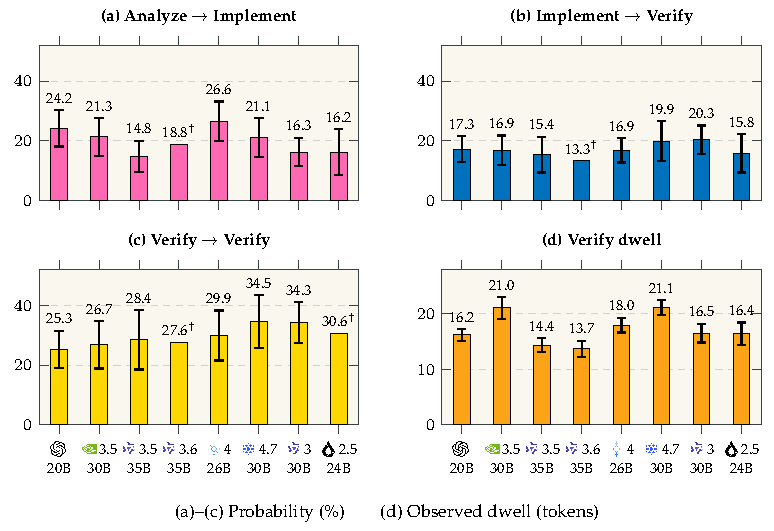
\includegraphics[width=\linewidth]{figures/journal/transition_summary.pdf}
\caption{Observed transitions from Analyze to Implement (a), Implement to Verify (b), and Verify to Verify (c), with Verify dwell (d).
%
Transition panels share a percentage scale.
%
Dwell counts labelled tokens in an observed run and can be censored by missing-label boundaries.
%
Horizontal values give means.
%
Whiskers show the whole-family-bootstrap, model-specific simultaneous 95\% intervals.
%
A dagger marks unavailable transition intervals.
%
These endpoints describe observed state dynamics.}
\label{fig:transition-summary}
\end{figure}

% Necessary local flush: the state/dwell figure must remain in Appendix C.
\FloatBarrier
\journalappendix{Benchmark Denominators and Model Configurations}{app:benchmark-details}

The complete native score table retains all six benchmark cells for every evaluated model (Table~\ref{tab:benchmark-details}).
%
The intervals are the original source-question bootstrap intervals.
%
The 32 attempts for each competition question remain dependent measurements, and unresolved answers are excluded from the scored denominator.
%

% Multipage longtable: retained outside adjustbox so page breaks remain available.
% Compact 2pt intercolumn spacing fits the full model identities without text scaling.
% Adapted from SPSD tab:main-results and SYNCO tab:mainRes.
\begingroup\small
\setlength{\tabcolsep}{2pt}
\begin{longtable}{llrrc}
\caption{\protect\phantomsection\label{tab:benchmark-details}Mean native card-profile accuracy (\%) with question-bootstrap 95\% confidence intervals in subscripts.
%
Repeated attempts remain grouped by source question.
%
Scored counts retain unresolved-answer exclusions.
%
Bold and underline mark the highest and second-highest unrounded means per benchmark, with ties sharing a rank, as in Table~\ref{tab:benchmarks}.}\\
\toprule
Model & Benchmark & Questions & Scored & Mean accuracy (\%) \\
\midrule\endfirsthead
\multicolumn{5}{l}{\textit{Continued}}\\
\toprule
Model & Benchmark & Questions & Scored & Mean accuracy (\%) \\
\midrule\endhead
\bottomrule\endfoot
\modelname{openai}{GPT-OSS-20B} & AIME24 & 30 & 956 & \cid{78.7}{13.0}{9.7} \\
\modelname{openai}{GPT-OSS-20B} & AIME25 & 30 & 956 & \cid{76.0}{11.4}{10.0} \\
\modelname{openai}{GPT-OSS-20B} & AMC23 & 40 & 1278 & \cid{97.3}{2.7}{2.1} \\
\modelname{openai}{GPT-OSS-20B} & MATH-500 & 500 & 500 & \cid{97.0}{1.6}{1.4} \\
\modelname{openai}{GPT-OSS-20B} & Minerva Math & 272 & 272 & \cid{69.1}{5.9}{5.5} \\
\modelname{openai}{GPT-OSS-20B} & OlympiadBench & 675 & 674 & \cid{83.2}{2.8}{2.7} \\
\modelname{nvidia}{\shortstack[l]{Nemotron-3.5-Lightning\\30B-A3B}} & AIME24 & 30 & 960 & \cid{87.8}{12.5}{8.8} \\
\modelname{nvidia}{\shortstack[l]{Nemotron-3.5-Lightning\\30B-A3B}} & AIME25 & 30 & 960 & \cid{87.2}{11.3}{9.2} \\
\modelname{nvidia}{\shortstack[l]{Nemotron-3.5-Lightning\\30B-A3B}} & AMC23 & 40 & 1280 & \secondcid{99.8}{0.3}{0.2} \\
\modelname{nvidia}{\shortstack[l]{Nemotron-3.5-Lightning\\30B-A3B}} & MATH-500 & 500 & 500 & \cid{98.8}{1.0}{0.8} \\
\modelname{nvidia}{\shortstack[l]{Nemotron-3.5-Lightning\\30B-A3B}} & Minerva Math & 272 & 272 & \cid{73.5}{5.9}{5.1} \\
\modelname{nvidia}{\shortstack[l]{Nemotron-3.5-Lightning\\30B-A3B}} & OlympiadBench & 675 & 675 & \cid{88.6}{2.4}{2.4} \\
\modelname{qwen}{Qwen3.5-35B-A3B} & AIME24 & 30 & 960 & \secondcid{94.0}{8.6}{5.4} \\
\modelname{qwen}{Qwen3.5-35B-A3B} & AIME25 & 30 & 960 & \cid{88.3}{11.3}{9.8} \\
\modelname{qwen}{Qwen3.5-35B-A3B} & AMC23 & 40 & 1280 & \bestcid{100.0}{0.0}{0.0} \\
\modelname{qwen}{Qwen3.5-35B-A3B} & MATH-500 & 500 & 500 & \secondcid{99.4}{0.8}{0.6} \\
\modelname{qwen}{Qwen3.5-35B-A3B} & Minerva Math & 272 & 271 & \cid{73.4}{5.5}{5.5} \\
\modelname{qwen}{Qwen3.5-35B-A3B} & OlympiadBench & 675 & 675 & \bestcid{92.3}{2.1}{2.1} \\
\modelname{qwen}{Qwen3.6-35B-A3B} & AIME24 & 30 & 960 & \bestcid{94.8}{7.1}{5.0} \\
\modelname{qwen}{Qwen3.6-35B-A3B} & AIME25 & 30 & 960 & \bestcid{89.7}{10.9}{9.2} \\
\modelname{qwen}{Qwen3.6-35B-A3B} & AMC23 & 40 & 1280 & \bestcid{100.0}{0.0}{0.0} \\
\modelname{qwen}{Qwen3.6-35B-A3B} & MATH-500 & 500 & 500 & \bestcid{99.6}{0.6}{0.4} \\
\modelname{qwen}{Qwen3.6-35B-A3B} & Minerva Math & 272 & 270 & \secondcid{74.8}{5.6}{5.2} \\
\modelname{qwen}{Qwen3.6-35B-A3B} & OlympiadBench & 675 & 675 & \secondcid{92.0}{2.1}{1.9} \\
\modelname{gemma}{Gemma-4-26B-A4B} & AIME24 & 30 & 959 & \cid{90.8}{9.8}{7.2} \\
\modelname{gemma}{Gemma-4-26B-A4B} & AIME25 & 30 & 948 & \cid{86.8}{10.5}{8.8} \\
\modelname{gemma}{Gemma-4-26B-A4B} & AMC23 & 40 & 1280 & \cid{99.7}{0.6}{0.3} \\
\modelname{gemma}{Gemma-4-26B-A4B} & MATH-500 & 500 & 500 & \cid{99.0}{1.0}{0.8} \\
\modelname{gemma}{Gemma-4-26B-A4B} & Minerva Math & 272 & 271 & \bestcid{75.6}{4.8}{5.2} \\
\modelname{gemma}{Gemma-4-26B-A4B} & OlympiadBench & 675 & 674 & \cid{90.8}{2.2}{2.1} \\
\modelname{zhipu}{GLM-4.7-Flash (30B-A3B)} & AIME24 & 30 & 960 & \cid{93.2}{7.7}{4.9} \\
\modelname{zhipu}{GLM-4.7-Flash (30B-A3B)} & AIME25 & 30 & 960 & \secondcid{89.6}{9.7}{7.6} \\
\modelname{zhipu}{GLM-4.7-Flash (30B-A3B)} & AMC23 & 40 & 1280 & \cid{99.4}{0.5}{0.4} \\
\modelname{zhipu}{GLM-4.7-Flash (30B-A3B)} & MATH-500 & 500 & 500 & \cid{98.4}{1.2}{1.0} \\
\modelname{zhipu}{GLM-4.7-Flash (30B-A3B)} & Minerva Math & 272 & 271 & \cid{73.1}{5.5}{5.2} \\
\modelname{zhipu}{GLM-4.7-Flash (30B-A3B)} & OlympiadBench & 675 & 674 & \cid{90.5}{2.2}{2.1} \\
\modelname{qwen}{Qwen3-30B-A3B} & AIME24 & 30 & 960 & \cid{80.2}{14.7}{11.0} \\
\modelname{qwen}{Qwen3-30B-A3B} & AIME25 & 30 & 960 & \cid{71.1}{13.3}{12.1} \\
\modelname{qwen}{Qwen3-30B-A3B} & AMC23 & 40 & 1280 & \cid{97.7}{2.5}{1.8} \\
\modelname{qwen}{Qwen3-30B-A3B} & MATH-500 & 500 & 500 & \cid{98.0}{1.2}{1.2} \\
\modelname{qwen}{Qwen3-30B-A3B} & Minerva Math & 272 & 271 & \bestcid{75.6}{5.2}{4.8} \\
\modelname{qwen}{Qwen3-30B-A3B} & OlympiadBench & 675 & 674 & \cid{84.6}{2.8}{2.5} \\
\modelname{liquid}{LFM2.5-24B-A2B} & AIME24 & 30 & 960 & \cid{86.9}{12.3}{8.4} \\
\modelname{liquid}{LFM2.5-24B-A2B} & AIME25 & 30 & 960 & \cid{84.4}{9.9}{8.6} \\
\modelname{liquid}{LFM2.5-24B-A2B} & AMC23 & 40 & 1280 & \cid{97.9}{2.3}{1.7} \\
\modelname{liquid}{LFM2.5-24B-A2B} & MATH-500 & 500 & 500 & \cid{98.8}{1.0}{0.8} \\
\modelname{liquid}{LFM2.5-24B-A2B} & Minerva Math & 272 & 271 & \cid{74.2}{5.7}{5.2} \\
\modelname{liquid}{LFM2.5-24B-A2B} & OlympiadBench & 675 & 675 & \cid{89.0}{2.5}{2.2} \\
\end{longtable}
\endgroup


\subsection{Model identities}
The evaluated models are OpenAI's GPT-OSS-20B, NVIDIA's Nemotron-3.5-Lightning-30B-A3B-NVFP4, Qwen3.5-35B-A3B-GPTQ-Int4, Qwen3.6-35B-A3B-FP8, NVIDIA's Gemma-4-26B-A4B-NVFP4, Z.ai's GLM-4.7-Flash, Qwen3-30B-A3B, and LiquidAI's LFM2.5-24B-A2B.
%
The native evaluation retains their model-specific tokenizers and reasoning parsers.
%
GPT-OSS has a 131,072-token context capacity.
%
The retained five long-context profiles use 133,120 tokens, while Qwen3-30B uses 40,960.
%
Its output cap is 38,912 tokens.
%
The five long-context card profiles have a 131,072-token output cap, and GPT-OSS output is bounded by the remaining context.
%
LFM2.5 runs in BF16 with a 131,072-token context, and its output is bounded by the remaining context.
%
Its 38 routed layers follow two dense layers and use sigmoid selection scores with a correction bias.
%

\subsection{Native benchmark prompt}
\label{app:native-prompt}

The eight evaluated models receive the same user-message template for these benchmarks.
%
The problem text replaces the italicized field.
%
\begin{quote}\small
Please reason step by step, and put your final answer within \verb|\boxed{}|.\\ Question: \emph{problem text}
\end{quote}
There are no few-shot examples or separate system messages.
%
Each model uses its native chat template.
%
Gemma and LFM2.5 explicitly enable thinking, and GPT-OSS uses medium reasoning effort.
%
The other profiles retain their native thinking settings without a template override.
%
These conditions describe the completed native evaluation.
%

\journalappendix{Annotation and External Prefix Probes}{app:annotation}

\subsection{Native sentence sampling and token alignment}

Native reasoning regions are identified using each model's reasoning delimiters.
%
A deterministic punctuation/newline splitter protects mathematical expressions and records exact character offsets.
%
It splits the reasoning region into sentence units, rather than applying a learned linguistic parser.
%
A completion token belongs to the sentence with greatest character overlap.
%
Ties choose the earlier sentence, and whitespace gaps attach to the preceding sentence.
%
Delimiter and answer tokens have no sentence owner.
%

One uniformly sampled attempt per question defines the native allocation population.
%
Within those attempts, the annotation floor samples up to ten sentences without replacement.
%
Remaining assignments sample the pooled unused sentences toward the 100,000-unit budget.
%
A separate competition sample includes up to four successful and four unsuccessful attempts from questions having at least two of each.
%
It assigns up to 60 sentences per attempt.
%
When an attempt overlaps the allocation population, its sentence assignments are unioned, so the available union can exceed the nominal budget.
%
Unscored attempts are not assigned to its success/failure strata.
%
The allocation comparison continues to use its original single sampled attempt per question.
%
Unassigned, invalid or unavailable labels remain missing and break sentence adjacency.
%

\subsection{External annotation development}

The external annotation development corpus contains 38 released DeepSeek-R1 SAT responses and 3,125 labelled units.
%
Complete responses define the partitions before units are flattened.
%
The Qwen3.8 seed deployment check uses 407 reused validation units, obtaining accuracy 0.710 under both low and medium effort.
%
The settings change 41 labels, or 10.1\% of those units.
%
Equal aggregate accuracy therefore does not imply an unchanged set of individual judgments.
%

The retained prompt has balanced accuracy 0.7400 in its selection comparison, against 0.7288 for the optimized candidate.
%
The Plan-recall gate retains the seed.
%
An earlier response-grouped, static-reward prompt study obtains macro-F1 0.6505 with a light optimization budget and 0.6437 with a heavy budget over 2,789 units.
%
These are different development comparisons, and their scores do not supply native seven-model annotation accuracy.
%

\subsection{Lexical reading of intervention continuations}
\label{app:lexical-readout}

The state of an intervention continuation is assigned by a text classifier rather than by the annotation reader.
%
It receives the sentence and its two neighbours, the same text the reader sees apart from the problem statement.
%
Word unigrams and bigrams and character 3- to 5-grams of the sentence, and word unigrams and bigrams of each neighbour, enter as hashed sublinear TF-IDF blocks fitted on the training rows.
%
The neighbour blocks carry half the weight of the sentence block, and nine format features record length, digit and symbol density, closing question marks or colons, bullets, and the response-boundary markers.
%
A multinomial logistic regression with an $L_2$ penalty maps these features to the seven classes.
%

Training uses the reader-labelled native sentences of the seven source models, at most 60,000 unique contexts per model and 420,000 in total.
%
Each evaluation fold has its own classifier, fitted on the families of the other four folds, so no continuation is read by a classifier that saw its question family.
%
On held-out native sentences the classifier agrees with the reader on 73.4\% of labels, with macro-F1 0.696 and per-model accuracy between 72.0\% and 75.0\%.
%
Its Youden index, sensitivity minus false-positive rate, ranges from 0.42 for Read to 0.74 for Implement.
%
The reader itself agrees with a repeated judgment of the same context in 83 to 95\% of duplicated contexts, which bounds the agreement any reader-trained classifier can reach.
%
LFM2.5 contributes no training sentence.
%
On its 96,137 reader-labelled native contexts, the same fold-specific classifiers agree with the reader on 72.7\% of labels, with macro-F1 0.672 and Youden indices between 0.37 for Read and 0.74 for Implement.
%

Non-differential classification errors shrink a contrast in class occupancy by the Youden index of that class without changing its sign.
%
The main analysis therefore reports uncorrected occupancy contrasts and gives Rogan--Gladen corrections, which divide by the native Youden index, as a sensitivity analysis.
%
On 27,746 reader-labelled sentences from an earlier steering study, an equivalent classifier reaches 74.4\% agreement, and its accuracy differs between targeted and random arms by 0.3 points with a 95\% interval from $-0.8$ to $1.4$.
%
Classifier contrasts between those arms correlate with reader contrasts at $r=0.71$, with a slope consistent with the Youden attenuation.
%
These checks cover a single model and milder edits, so the readout supports statements about lexical signatures of the reasoning classes rather than independently verified cognitive states.
%

\subsection{Prospective hidden-state information}
\label{app:probes}

The external prefix-probe study removes 38 synthetic closing-think units, leaving 3,087 annotated units.
%
The feature for a sentence is the hidden state immediately before its first token.
%
Each encoder receives the released response as a teacher-forced continuation.
%
The probe therefore observes the problem and preceding text without the target sentence.
%

The probes use balanced one-versus-rest logistic regression with L2 regularization, $C=1$, and raw hidden activations without standardization or principal-component reduction.
%
Five common response-disjoint outer folds hold out complete responses.
%
Inner validation selects the layer for each one-versus-rest target by area under the receiver operating characteristic curve (AUROC), and the selected classifier is refitted on the outer development responses.
%
A position-only baseline uses the logarithms of preceding unit and token counts, without future content or final response length.
%

\begin{table}[htbp]
\centering\small
\caption{Response-disjoint prospective probes on 38 SAT responses.
%
AUROC averages the five folds and seven binary targets.
%
Subscripts give $\pm$ 95\% response-bootstrap confidence intervals, conditional on the saved folds, layers, and fits.
%
Gain subtracts the position baseline.
%
Bold and underline identify the highest and second-highest distinct probe AUROC and paired gain.
%
Probes use encoder-specific representations.}
\label{tab:prefix-probes}
\begin{adjustbox}{max width=\linewidth}
\begin{tabular}{@{}lrrr@{}}
\toprule
Encoder & Probe AUROC & Position AUROC & Paired gain \\
\midrule
\modelname{qwen}{Qwen3.5-35B-A3B} & \bestcid{0.852}{0.014}{0.016} & \cid{0.566}{0.014}{0.028} & \bestcid{0.286}{0.027}{0.016} \\
\modelname{openai}{GPT-OSS-20B} & \cid{0.780}{0.019}{0.017} & \cid{0.571}{0.014}{0.029} & \cid{0.209}{0.030}{0.018} \\
\modelname{gemma}{Gemma-4-26B-A4B} & \secondcid{0.788}{0.016}{0.017} & \cid{0.566}{0.013}{0.028} & \secondcid{0.221}{0.026}{0.016} \\
\bottomrule
\end{tabular}
\end{adjustbox}
\end{table}

Every encoder exceeds its position baseline (Table~\ref{tab:prefix-probes}).
%
The intervals resample whole responses and condition on the chosen layers and fitted classifiers.
%
They omit refitting and split-seed variation.
%
Macro binary F1 is 0.521 for Qwen3.5, 0.400 for GPT-OSS, and 0.426 for Gemma at the retained decision rule.
%
Ranking information does not therefore establish reliable seven-class annotation of a model's own generated solutions.
%

\subsection{Candidate-specific verification qualification}
\label{app:verification-qualification}

The separate prospective verification protocol recognizes a checkable candidate value inside an already emitted reasoning prefix.
%
Its frozen qualification combines family support, precision, and evidence of whether that candidate has already been checked.
%
The completed recognition audits do not qualify in five models.
%
Qwen3.5 and GLM remain incomplete under that protocol (Table~\ref{tab:verification-qualification}).
%
No new targeted-control outcome is measured for these seven protocol cells.
%

\begin{table}[htb]
\centering\small
\caption{Qualification of the separate candidate-specific verification protocol.
%
Engineering qualification concerns execution.
%
Recognition and targeted-control outcomes are assessed separately.}
\label{tab:verification-qualification}
\begin{adjustbox}{max width=\linewidth}
\begin{tabular}{@{}llll@{}}
\toprule
Model & Engineering & Recognition & Targeted control \\
\midrule
\modelname{openai}{GPT-OSS-20B} & Qualified & Criterion unmet & Unmeasured \\
\modelname{nvidia}{\shortstack[l]{Nemotron-3.5-Lightning\\30B-A3B}} & Qualified & Criterion unmet & Unmeasured \\
\modelname{qwen}{Qwen3.5-35B-A3B} & Qualified & Incomplete & Unmeasured \\
\modelname{qwen}{Qwen3.6-35B-A3B} & Qualified & Criterion unmet & Unmeasured \\
\modelname{gemma}{Gemma-4-26B-A4B} & Qualified & Criterion unmet & Unmeasured \\
\modelname{zhipu}{GLM-4.7-Flash (30B-A3B)} & Qualified & Incomplete & Unmeasured \\
\modelname{qwen}{Qwen3-30B-A3B} & Qualified & Criterion unmet & Unmeasured \\
\bottomrule
\end{tabular}
\end{adjustbox}
\end{table}

GPT-OSS's complete audit has 128 prefix assignments and two original reader draws per assignment.
%
Apparent eligibility precision is 22.41\% across 29 families, and already-checked precision is 18.75\% across eight families.
%
The frozen thresholds are 70\% precision and ten families for each qualification.
%
Both measured precisions fall below that criterion, and already-checked support also falls below ten families.
%
These results limit this recognition procedure's applicability.
%
An unmeasured control outcome does not estimate a causal null.

% Necessary local flush: the qualification float belongs to Appendix E.
\FloatBarrier
\journalappendix{Exploratory Correctness Associations}{app:associations}

An exploratory analysis relates whole-reasoning use of class-enriched expert sets to adjudicated correctness.
%
The retained rule nominates up to three experts per selected layer for each class on the full allocation corpus, without using correctness to rank them.
%
Their selected-slot use is measured over all reasoning tokens, including tokens outside the class used for nomination.
%
The class sets can overlap.
%

The original partial Pearson correlations adjust for benchmark, log completion length, retrospective difficulty, the labelled class's token share, and a cap indicator when present.
%
Difficulty uses other attempts on repeated competition questions or the other models on single-attempt benchmarks.
%
It is a retrospective adjustment variable.
%

The strongest corrected associations occur in Qwen3.5 and Qwen3.6.
%
Analyze-profile use has $r=0.0918$ and $r=0.0818$, while Verify-profile use has $r=-0.0972$ and $r=-0.1008$.
%
The Monitor-profile correlations are $-0.0770$ and $-0.0995$.
%
Nemotron's Monitor association is $-0.0853$.
%
The remaining tested mean-feature associations do not pass the original corrected threshold.
%

That threshold applies Benjamini--Hochberg correction within each model's 21 mean-feature comparisons~\citep{benjamini1995fdr}.
%
The original intervals use 1,000 question-ID bootstrap draws, refitting nuisance regressions while holding nominated sets and difficulty fixed.
%
They do not cluster duplicate families.
%
This is same-cohort association evidence.
%
It does not supply held-out expert usefulness or the effect of removing a class-associated expert.
%

\journalappendix{Paired Routing Interventions}{app:routing-levels}

Table~\ref{tab:routing-levels} gives the accuracy and token levels behind the paired contrasts of Section~\ref{sec:routing-results}.
%
Native routing ends naturally in at least 98\% of continuations in every model, and no edited arm changes this share by more than one point.
%
The levels carry wider intervals than the paired contrasts because they retain the variation between families that pairing removes.
%

% Multipage longtable: retained outside adjustbox so page breaks remain available.
% Source: analysis-final/EFFECTS.json levels_by_model via scripts/paper/export_routing_results.py.
\begingroup\small
\setlength{\tabcolsep}{2pt}
\begin{longtable}{lcccc}
\caption{Accuracy and token levels of every intervention arm, with family-bootstrap simultaneous 95\% confidence intervals as subscripts.
%
Accuracy is strict answer scoring of the completed continuation.
%
Generated tokens follow the frozen prefix, and reasoning tokens are the generated tokens before the reasoning closes.
%
Random arms use the matched control sets, and natural end is the share of continuations that stop before their original generation allowance.
%
Benchmarks and supported families receive equal weight, and intervals are simultaneous over the arm and metric cells of each model.}\label{tab:routing-levels}\\
\toprule
Arm & Accuracy (\%) & Generated tokens & Reasoning tokens & Natural end (\%) \\
\midrule\endfirsthead
\multicolumn{5}{l}{\textit{Continued}}\\
\toprule
Arm & Accuracy (\%) & Generated tokens & Reasoning tokens & Natural end (\%) \\
\midrule\endhead
\bottomrule\endfoot
\multicolumn{5}{l}{\modelname{openai}{GPT-OSS-20B}}\\*
Native & \cid{78.06}{9.18}{9.18} & \cid{3838}{1429}{1429} & \cid{3340}{1409}{1409} & \cid{100.0}{0.0}{0.0} \\*
Targeted activation & \cid{77.18}{8.17}{8.17} & \cid{3735}{1142}{1142} & \cid{3258}{1128}{1128} & \cid{100.0}{0.0}{0.0} \\*
Random activation & \cid{77.74}{8.13}{8.13} & \cid{3758}{1127}{1127} & \cid{3284}{1112}{1112} & \cid{100.0}{0.0}{0.0} \\*
Targeted deactivation & \cid{75.95}{8.34}{8.34} & \cid{3726}{1188}{1188} & \cid{3258}{1175}{1175} & \cid{100.0}{0.0}{0.0} \\*
Random deactivation & \cid{75.95}{8.22}{8.22} & \cid{3672}{1225}{1225} & \cid{3217}{1202}{1202} & \cid{100.0}{0.0}{0.0} \\
\midrule
\multicolumn{5}{l}{\modelname{nvidia}{Nemotron-3.5-Lightning-30B-A3B}}\\*
Native & \cid{84.73}{7.37}{7.37} & \cid{8034}{2846}{2846} & \cid{7675}{2853}{2853} & \cid{100.0}{0.0}{0.0} \\*
Targeted activation & \cid{84.53}{6.82}{6.82} & \cid{7363}{2390}{2390} & \cid{6986}{2395}{2395} & \cid{100.0}{0.0}{0.0} \\*
Random activation & \cid{83.46}{7.09}{7.09} & \cid{7632}{2597}{2597} & \cid{7257}{2602}{2602} & \cid{100.0}{0.0}{0.0} \\*
Targeted deactivation & \cid{83.94}{7.12}{7.12} & \cid{7763}{2613}{2613} & \cid{7392}{2619}{2619} & \cid{100.0}{0.0}{0.0} \\*
Random deactivation & \cid{83.62}{7.00}{7.00} & \cid{7416}{2464}{2464} & \cid{7044}{2468}{2468} & \cid{100.0}{0.0}{0.0} \\
\midrule
\multicolumn{5}{l}{\modelname{qwen}{Qwen3.5-35B-A3B}}\\*
Native & \cid{87.78}{7.12}{7.12} & \cid{9838}{2580}{2580} & \cid{8890}{2610}{2610} & \cid{100.0}{0.0}{0.0} \\*
Targeted activation & \cid{87.22}{6.76}{6.76} & \cid{10442}{2945}{2945} & \cid{9470}{2960}{2960} & \cid{100.0}{0.0}{0.0} \\*
Random activation & \cid{87.46}{7.04}{7.04} & \cid{10288}{2746}{2746} & \cid{9326}{2747}{2747} & \cid{99.9}{0.2}{0.2} \\*
Targeted deactivation & \cid{87.02}{7.03}{7.03} & \cid{10252}{2787}{2787} & \cid{9270}{2792}{2792} & \cid{100.0}{0.0}{0.0} \\*
Random deactivation & \cid{87.54}{7.02}{7.02} & \cid{9954}{2769}{2769} & \cid{8991}{2779}{2779} & \cid{100.0}{0.0}{0.0} \\
\midrule
\multicolumn{5}{l}{\modelname{qwen}{Qwen3.6-35B-A3B}}\\*
Native & \cid{87.50}{6.29}{6.29} & \cid{11828}{3464}{3464} & \cid{11149}{3461}{3461} & \cid{100.0}{0.0}{0.0} \\*
Targeted activation & \cid{85.79}{7.01}{7.01} & \cid{11273}{3395}{3395} & \cid{10597}{3390}{3390} & \cid{99.8}{0.4}{0.4} \\*
Random activation & \cid{86.39}{6.84}{6.84} & \cid{11806}{4065}{4065} & \cid{11133}{4066}{4066} & \cid{99.5}{1.2}{1.2} \\*
Targeted deactivation & \cid{86.27}{6.42}{6.42} & \cid{11633}{3978}{3978} & \cid{10961}{3980}{3980} & \cid{99.2}{2.0}{2.0} \\*
Random deactivation & \cid{85.87}{6.56}{6.56} & \cid{11532}{4007}{4007} & \cid{10856}{4005}{4005} & \cid{99.4}{1.6}{1.6} \\
\midrule
\multicolumn{5}{l}{\modelname{gemma}{Gemma-4-26B-A4B}}\\*
Native & \cid{85.83}{7.57}{7.57} & \cid{8278}{4156}{4156} & \cid{7519}{4186}{4186} & \cid{98.1}{3.9}{3.9} \\*
Targeted activation & \cid{84.88}{7.53}{7.53} & \cid{7735}{2733}{2733} & \cid{6959}{2743}{2743} & \cid{98.5}{2.3}{2.3} \\*
Random activation & \cid{83.85}{7.57}{7.57} & \cid{8091}{3335}{3335} & \cid{7016}{3258}{3258} & \cid{98.0}{2.7}{2.7} \\*
Targeted deactivation & \cid{84.05}{7.43}{7.43} & \cid{8141}{2999}{2999} & \cid{7389}{3019}{3019} & \cid{98.1}{2.3}{2.3} \\*
Random deactivation & \cid{84.44}{7.54}{7.54} & \cid{7679}{2556}{2556} & \cid{6920}{2572}{2572} & \cid{98.4}{2.1}{2.1} \\
\midrule
\multicolumn{5}{l}{\modelname{zhipu}{GLM-4.7-Flash (30B-A3B)}}\\*
Native & \cid{85.00}{7.48}{7.48} & \cid{9093}{3432}{3432} & \cid{8638}{3437}{3437} & \cid{98.3}{2.5}{2.5} \\*
Targeted activation & \cid{84.64}{7.13}{7.13} & \cid{9139}{3687}{3687} & \cid{8705}{3683}{3683} & \cid{98.5}{2.3}{2.3} \\*
Random activation & \cid{84.76}{6.66}{6.66} & \cid{9094}{3792}{3792} & \cid{8670}{3793}{3793} & \cid{98.4}{2.4}{2.4} \\*
Targeted deactivation & \cid{84.64}{7.32}{7.32} & \cid{9425}{3785}{3785} & \cid{9000}{3783}{3783} & \cid{98.3}{2.3}{2.3} \\*
Random deactivation & \cid{84.76}{7.02}{7.02} & \cid{9368}{3602}{3602} & \cid{8948}{3602}{3602} & \cid{98.3}{2.3}{2.3} \\
\midrule
\multicolumn{5}{l}{\modelname{qwen}{Qwen3-30B-A3B}}\\*
Native & \cid{79.73}{9.81}{9.81} & \cid{6130}{1403}{1403} & \cid{5305}{1392}{1392} & \cid{99.4}{1.5}{1.5} \\*
Targeted activation & \cid{78.57}{9.02}{9.02} & \cid{6554}{1430}{1430} & \cid{5741}{1418}{1418} & \cid{99.0}{1.9}{1.9} \\*
Random activation & \cid{77.95}{9.60}{9.60} & \cid{6411}{1433}{1433} & \cid{5607}{1430}{1430} & \cid{99.4}{1.5}{1.5} \\*
Targeted deactivation & \cid{77.67}{9.76}{9.76} & \cid{6399}{1376}{1376} & \cid{5582}{1369}{1369} & \cid{98.9}{1.8}{1.8} \\*
Random deactivation & \cid{78.26}{9.04}{9.04} & \cid{6308}{1322}{1322} & \cid{5488}{1304}{1304} & \cid{99.4}{1.5}{1.5} \\
\midrule
\multicolumn{5}{l}{\modelname{liquid}{LFM2.5-24B-A2B}}\\*
Native & \cid{85.43}{8.23}{8.23} & \cid{9706}{5597}{5597} & \cid{9384}{5608}{5608} & \cid{99.4}{1.7}{1.7} \\*
Targeted activation & \cid{84.37}{7.73}{7.73} & \cid{8637}{5018}{5018} & \cid{8319}{5033}{5033} & \cid{99.0}{1.8}{1.8} \\*
Random activation & \cid{83.93}{7.81}{7.81} & \cid{9620}{4846}{4846} & \cid{9304}{4856}{4856} & \cid{99.0}{1.9}{1.9} \\*
Targeted deactivation & \cid{84.01}{7.56}{7.56} & \cid{8856}{4310}{4310} & \cid{8534}{4322}{4322} & \cid{98.8}{1.9}{1.9} \\*
Random deactivation & \cid{84.76}{7.44}{7.44} & \cid{8464}{4378}{4378} & \cid{8138}{4390}{4390} & \cid{99.1}{1.8}{1.8} \\
\end{longtable}
\endgroup


\subsection{Pre-registered efficiency link}
\label{app:efficiency-link}

The efficiency link was frozen on native traces before any intervention outcome existed.
%
For each model and class, a regression of the log remaining reasoning tokens on the class indicator absorbs question and absolute-position fixed effects, without relative position or trace effects that would leak the outcome (Table~\ref{tab:efficiency-link}).
%
Its intervals use 2,000 family-bootstrap resamples with seed 20261017, shared across models, classes and outcomes.
%
The prediction states that the token effect of targeted activation relative to matched random activation correlates positively with this coefficient across model--class cells, and that the accuracy effect correlates positively with the corresponding correctness coefficient.
%
The test reports the Spearman correlation and the sign-agreement rate over cells whose native interval excludes zero.
%
LFM2.5 has no frozen coefficient because its labels became available after the pre-registration.
%

% Source: report/final-routing-20261015-r1/driver/EFFICIENCY_LINK_PREREG.json via scripts/paper/export_routing_results.py.
\begin{table}[tb]
\centering\small
\caption{Pre-registered native association between the current reasoning state and the remaining reasoning length, with 95\% family-bootstrap confidence intervals as subscripts.
%
Entries are 100 times the regression coefficient of a class indicator on the log of the reasoning tokens that remain after the sentence, with question and absolute-position fixed effects.
%
Negative values mark states followed by shorter remaining reasoning.
%
The coefficients were frozen before any intervention outcome existed.}
\label{tab:efficiency-link}
\setlength{\tabcolsep}{2pt}
\begin{adjustbox}{max width=\linewidth}
\begin{tabular}{@{}lccccccc@{}}
\toprule
Model & \textrm{Re} & \textrm{An} & \textrm{Ex} & \textrm{Pl} & \textrm{Im} & \textrm{Ve} & \textrm{Mo} \\
\midrule
\modelname{openai}{GPT-OSS-20B} & \cid{19.88}{2.60}{2.82} & \cid{11.58}{1.65}{1.82} & \cid{4.56}{1.67}{1.76} & \cid{8.98}{2.01}{2.00} & \cid{0.71}{1.81}{1.81} & \cid{-4.69}{1.93}{1.91} & \cid{-36.71}{3.74}{3.53} \\
\modelname{nvidia}{Nemotron-3.5-Lightning-30B-A3B} & \cid{10.43}{2.82}{2.93} & \cid{6.61}{1.21}{1.21} & \cid{0.22}{1.38}{1.45} & \cid{8.05}{1.65}{1.72} & \cid{2.81}{1.71}{1.70} & \cid{-4.79}{1.82}{1.73} & \cid{-30.76}{4.00}{3.83} \\
\modelname{qwen}{Qwen3.5-35B-A3B} & \cid{1.78}{2.22}{2.15} & \cid{4.09}{1.18}{1.15} & \cid{1.86}{1.60}{1.53} & \cid{4.01}{2.05}{2.11} & \cid{1.02}{1.47}{1.43} & \cid{-5.01}{1.66}{1.71} & \cid{-8.95}{1.95}{2.04} \\
\modelname{qwen}{Qwen3.6-35B-A3B} & \cid{-0.93}{2.47}{2.40} & \cid{5.57}{1.12}{1.25} & \cid{0.78}{1.39}{1.42} & \cid{4.06}{2.09}{1.99} & \cid{2.21}{1.45}{1.47} & \cid{-5.24}{1.90}{1.84} & \cid{-11.12}{1.81}{1.83} \\
\modelname{gemma}{Gemma-4-26B-A4B} & \cid{4.57}{2.06}{2.08} & \cid{5.91}{1.34}{1.36} & \cid{3.38}{2.06}{2.20} & \cid{4.07}{2.45}{2.58} & \cid{-2.35}{1.48}{1.42} & \cid{-7.57}{1.83}{1.75} & \cid{-3.40}{2.80}{2.77} \\
\modelname{zhipu}{GLM-4.7-Flash (30B-A3B)} & \cid{19.12}{3.81}{3.80} & \cid{7.43}{1.56}{1.69} & \cid{1.78}{1.97}{1.89} & \cid{2.02}{2.29}{2.38} & \cid{2.97}{1.96}{1.92} & \cid{-3.66}{1.78}{1.70} & \cid{-28.28}{3.77}{3.42} \\
\modelname{qwen}{Qwen3-30B-A3B} & \cid{4.60}{1.75}{1.81} & \cid{8.20}{1.24}{1.32} & \cid{4.51}{1.52}{1.41} & \cid{7.39}{1.40}{1.44} & \cid{2.46}{1.36}{1.36} & \cid{-6.88}{1.49}{1.46} & \cid{-18.32}{2.31}{2.22} \\
\midrule
Seven-model mean & \cid{8.49}{1.23}{1.31} & \cid{7.06}{0.57}{0.59} & \cid{2.44}{0.65}{0.65} & \cid{5.51}{0.82}{0.84} & \cid{1.40}{0.70}{0.67} & \cid{-5.41}{0.72}{0.71} & \cid{-19.65}{1.53}{1.36} \\
\bottomrule
\end{tabular}
\end{adjustbox}
\end{table}


Verify and Monitor precede shorter remaining reasoning in every model, and Analyze precedes longer remaining reasoning in every model.
%
The correctness coefficients are small, and only 20\% of the 49 cells exclude zero.
%
Neither prediction holds: the token correlation is $-0.11$, with a 95\% interval from $-0.29$ to $0.13$, and the accuracy correlation is $0.07$, from $-0.16$ to $0.31$.
%
Fixed effects for benchmark, total tokens instead of reasoning tokens, and accuracy restricted to completed traces give the same conclusion.
%

\subsection{Exploratory strong-dose arm}
\label{app:routing-strong}

The strong-dose arm was specified after the primary contrasts of three models had been inspected.
%
It reuses each family's native prefix and seed, and forces the high-count nominated sets of all three depth regions throughout the analysis window rather than for a pulse.
%
Its matched control forces the corresponding high-count control sets of the same layers.
%
The arm adds 7,196 continuations in GPT-OSS, Nemotron, Qwen3-30B and Gemma (Table~\ref{tab:routing-strong}).
%

% Source: report/final-routing-20261015-r1/driver/analysis-strong/EFFECTS.json via scripts/paper/export_routing_results.py.
\begin{table}[tb]
\centering\small
\caption{Exploratory strong-dose activation, with family-bootstrap simultaneous 95\% confidence intervals as subscripts.
%
The arm forces the nominated high-count expert sets at all three depth regions throughout the analysis window and compares them with the matched high-count control sets.
%
State columns give targeted minus matched-random percentage points.
%
Accuracy is in percentage points and generated tokens in percent; efficiency contrasts are estimated on the pooled population only.}
\label{tab:routing-strong}
\setlength{\tabcolsep}{2.5pt}
\begin{adjustbox}{max width=\linewidth}
\begin{tabular}{@{}lcccccc@{}}
\toprule
 & \multicolumn{2}{c}{Target state (pp)} & \multicolumn{2}{c}{Targeted $-$ random} & \multicolumn{2}{c}{Accuracy $-$ native (pp)} \\
\cmidrule(lr){2-3}\cmidrule(lr){4-5}\cmidrule(lr){6-7}
Model & Occupancy & First & Acc.\ (pp) & Tokens (\%) & Targeted & Random \\
\midrule
\modelname{openai}{GPT-OSS-20B} & \cid{-0.19}{0.93}{0.93} & \cid{0.08}{1.58}{1.58} & \textemdash & \textemdash & \textemdash & \textemdash \\
\modelname{nvidia}{Nemotron-3.5-Lightning-30B-A3B} & \cid{0.02}{0.95}{0.95} & \cid{0.42}{1.67}{1.67} & \textemdash & \textemdash & \textemdash & \textemdash \\
\modelname{qwen}{Qwen3-30B-A3B} & \cid{0.09}{0.98}{0.98} & \cid{-0.02}{1.15}{1.15} & \textemdash & \textemdash & \textemdash & \textemdash \\
\modelname{gemma}{Gemma-4-26B-A4B} & \cid{0.23}{0.85}{0.85} & \cid{0.48}{0.88}{0.88} & \textemdash & \textemdash & \textemdash & \textemdash \\
\midrule
All four models & \cid{0.04}{0.46}{0.46} & \cid{0.27}{0.76}{0.76} & \cid{-0.17}{1.22}{1.22} & \cid{0.2}{3.1}{3.1} & \cid{-1.52}{2.18}{2.18} & \cid{-1.35}{2.37}{2.37} \\
\bottomrule
\end{tabular}
\end{adjustbox}
\end{table}


Neither occupancy nor the first sentence moves toward the forced class beyond the matched control.
%
Both forced arms lower mean accuracy relative to native routing, with simultaneous intervals that include zero.
%
Sustained routing edits therefore leave the state unchanged even when they persist across the whole window.
%

\journalappendix{Whole-Reasoning Steering}{app:whole}

This appendix details the whole-reasoning steering of Section~\ref{sec:whole-steering}.
%
Table~\ref{tab:whole-cells} gives the token and accuracy effect of every steered cell at each model's base strength, against matched random edits and against native routing.
%
Table~\ref{tab:whole-occupancy} gives the response $\rho$ of the steered state's occupancy, signed so that positive values move the state in the intended direction.
%
Table~\ref{tab:whole-levels} gives, for every model, strength and arm, the completed continuations, the share that reaches the length limit, the share of repeated 16-token windows, the mean generated tokens and the share of router positions at which the edit changed the selected experts.
%

Three design choices were fixed before any production outcome.
%
The pre-production check stopped a model only for breakdown, after its length-ratio criterion was removed, and GPT-OSS-20B and GLM-4.7-Flash ran their base continuations at half strength (Section~\ref{sec:whole-setup}).
%
The random experts are drawn separately at each strength, so the strength comparison varies the matched control together with the targeted set.
%

% Multipage longtable: retained outside adjustbox so page breaks remain available.
% Source: report/whole-reasoning-20261021-r14/analysis-combined/EFFECTS_WHOLE.json (cell_effects, levels) via scripts/paper/export_whole_results.py.
\begingroup\small
\setlength{\tabcolsep}{2pt}
\begin{longtable}{lccccc}
\caption{Effects of every steered cell at each model's base strength, with family-bootstrap simultaneous 95\% confidence intervals as subscripts.
%
Re, An, Ex, Pl, Im, Ve and Mo abbreviate Read, Analyze, Explore, Plan, Implement, Verify and Monitor.
%
A dagger marks the efficiency-directed cells that enter the primary contrast.
%
Tokens give the percent change in reasoning tokens, with negative values meaning fewer tokens, and accuracy differences are in percentage points, for targeted edits against matched random edits and against native routing.
%
Limit gives the share of the targeted continuations of each operation that reach the length limit.
%
Intervals are simultaneous over the six contrasts of each cell and cover the outcome bounds of unfinished continuations.
%
Each model is shown at its base strength, which is full except for GPT-OSS-20B and GLM-4.7-Flash at half.}\label{tab:whole-cells}\\
\toprule
 & \multicolumn{2}{c}{Targeted $-$ random} & \multicolumn{2}{c}{Targeted $-$ native} & \\
\cmidrule(lr){2-3}\cmidrule(lr){4-5}
Cell & Tokens (\%) & Acc.\ (pp) & Tokens (\%) & Acc.\ (pp) & Limit (\%) \\
\midrule\endfirsthead
\multicolumn{6}{l}{\textit{Continued}}\\
\toprule
 & \multicolumn{2}{c}{Targeted $-$ random} & \multicolumn{2}{c}{Targeted $-$ native} & \\
\cmidrule(lr){2-3}\cmidrule(lr){4-5}
Cell & Tokens (\%) & Acc.\ (pp) & Tokens (\%) & Acc.\ (pp) & Limit (\%) \\
\midrule\endhead
\bottomrule\endfoot
\multicolumn{6}{l}{\modelname{openai}{GPT-OSS-20B}, half strength} \\*
\textit{Promote} & & & & & 0.2 \\*
\quad \textrm{Re} & \cid{331.8}{194.2}{194.2} & \cid{-45.56}{13.31}{13.31} & \cid{697.0}{1652.6}{1652.6} & \cid{-50.69}{16.93}{16.93} &  \\*
\quad \textrm{An} & \cid{523.7}{714.6}{714.6} & \cid{-60.56}{13.45}{13.45} & \cid{859.9}{2354.1}{2354.1} & \cid{-60.56}{16.53}{16.53} &  \\*
\quad \textrm{Ex} & \cid{279.3}{160.1}{160.1} & \cid{-47.50}{12.76}{12.76} & \cid{564.4}{1339.9}{1339.9} & \cid{-46.25}{16.69}{16.69} &  \\*
\quad \textrm{Pl} & \cid{498.0}{312.8}{312.8} & \cid{-50.00}{13.73}{13.73} & \cid{902.3}{2073.7}{2073.7} & \cid{-52.08}{17.92}{17.92} &  \\*
\quad \textrm{Im} & \cid{-17.0}{40.8}{40.8} & \cid{5.00}{10.27}{10.27} & \cid{43.2}{281.4}{281.4} & \cid{6.25}{13.99}{13.99} &  \\*
\quad \textrm{Ve}$^{\dagger}$ & \cid{43.0}{1564.1}{1564.1} & \cid{4.44}{27.07}{27.07} & \cid{106.7}{1081.9}{1081.9} & \cid{-9.03}{23.01}{23.01} &  \\*
\quad \textrm{Mo}$^{\dagger}$ & \cid{178.9}{2530.1}{2530.1} & \cid{-16.11}{27.07}{27.07} & \cid{135.4}{1269.5}{1269.5} & \cid{-17.08}{24.96}{24.96} &  \\*
\textit{Suppress} & & & & & 0.0 \\*
\quad \textrm{Re}$^{\dagger}$ & \cid{-18.0}{419.0}{419.0} & \cid{-1.39}{19.01}{19.01} & \cid{-5.5}{459.6}{459.6} & \cid{1.94}{19.69}{19.69} &  \\*
\quad \textrm{An}$^{\dagger}$ & \cid{-0.4}{425.4}{425.4} & \cid{-1.25}{17.56}{17.56} & \cid{10.2}{396.5}{396.5} & \cid{-1.11}{18.14}{18.14} &  \\*
\quad \textrm{Ex}$^{\dagger}$ & \cid{-0.6}{432.6}{432.6} & \cid{10.28}{19.22}{19.22} & \cid{13.3}{393.5}{393.5} & \cid{4.17}{18.14}{18.14} &  \\*
\quad \textrm{Pl}$^{\dagger}$ & \cid{23.1}{761.1}{761.1} & \cid{-2.22}{19.21}{19.21} & \cid{17.5}{580.6}{580.6} & \cid{1.11}{18.54}{18.54} &  \\
\midrule
\multicolumn{6}{l}{\modelname{nvidia}{Nemotron-3.5-Lightning-30B-A3B}, full strength} \\*
\textit{Promote} & & & & & 0.0 \\*
\quad \textrm{Re} & \cid{6.9}{29.8}{29.8} & \cid{1.41}{6.06}{6.06} & \cid{0.0}{28.2}{28.2} & \cid{0.57}{3.65}{3.65} &  \\*
\quad \textrm{An} & \cid{-9.4}{51.8}{51.8} & \cid{-0.83}{10.25}{10.25} & \cid{-12.9}{48.1}{48.1} & \cid{-2.76}{9.49}{9.49} &  \\*
\quad \textrm{Ex} & \cid{4.3}{30.0}{30.0} & \cid{0.34}{6.42}{6.42} & \cid{-5.9}{20.8}{20.8} & \cid{-0.78}{6.46}{6.46} &  \\*
\quad \textrm{Pl} & \cid{-1.1}{33.5}{33.5} & \cid{-2.50}{5.16}{5.16} & \cid{5.0}{23.1}{23.1} & \cid{-3.61}{6.30}{6.30} &  \\*
\quad \textrm{Im} & \cid{4.5}{34.8}{34.8} & \cid{-0.24}{5.72}{5.72} & \cid{-4.4}{20.4}{20.4} & \cid{-1.93}{6.46}{6.46} &  \\*
\quad \textrm{Ve}$^{\dagger}$ & \cid{8.2}{14.7}{14.7} & \cid{0.57}{5.73}{5.73} & \cid{2.8}{12.9}{12.9} & \cid{-2.80}{5.48}{5.48} &  \\*
\quad \textrm{Mo}$^{\dagger}$ & \cid{-9.8}{14.8}{14.8} & \cid{-0.32}{4.25}{4.25} & \cid{-4.4}{14.3}{14.3} & \cid{-1.96}{4.77}{4.77} &  \\*
\textit{Suppress} & & & & & 8.6 \\*
\quad \textrm{Re}$^{\dagger}$ & \cid{-7.3}{18.7}{18.7} & \cid{-3.95}{7.76}{7.76} & \cid{12.2}{21.7}{21.7} & \cid{-12.54}{8.73}{8.73} &  \\*
\quad \textrm{An}$^{\dagger}$ & \cid{80.2}{52.8}{52.8} & \cid{-15.23}{10.92}{10.92} & \cid{121.6}{64.0}{64.0} & \cid{-20.57}{11.41}{11.41} &  \\*
\quad \textrm{Pl}$^{\dagger}$ & \cid{-29.5}{32.9}{32.9} & \cid{4.94}{11.26}{11.26} & \cid{-21.8}{38.4}{38.4} & \cid{-5.95}{8.68}{8.68} &  \\*
\quad \textrm{Im}$^{\dagger}$ & \cid{175.9}{1410.1}{1410.1} & \cid{-48.59}{24.96}{24.96} & \cid{290.2}{1980.1}{1980.1} & \cid{-58.61}{24.24}{24.24} &  \\
\midrule
\multicolumn{6}{l}{\modelname{qwen}{Qwen3.5-35B-A3B}, full strength} \\*
\textit{Promote} & & & & & 0.0 \\*
\quad \textrm{Re} & \cid{4.2}{1760.2}{1760.2} & \cid{0.97}{26.66}{26.66} & \cid{-14.2}{973.4}{973.4} & \cid{0.69}{23.84}{23.84} &  \\*
\quad \textrm{An} & \cid{25.4}{2789.6}{2789.6} & \cid{2.78}{27.36}{27.36} & \cid{-5.0}{1016.9}{1016.9} & \cid{0.14}{22.87}{22.87} &  \\*
\quad \textrm{Ex} & \cid{32.7}{2055.0}{2055.0} & \cid{2.64}{24.34}{24.34} & \cid{-4.5}{838.1}{838.1} & \cid{1.25}{21.08}{21.08} &  \\*
\quad \textrm{Pl} & \cid{-5.1}{1362.2}{1362.2} & \cid{0.69}{23.83}{23.83} & \cid{-17.6}{814.0}{814.0} & \cid{1.11}{22.40}{22.40} &  \\*
\quad \textrm{Im} & \cid{-1.6}{1545.7}{1545.7} & \cid{-0.14}{24.28}{24.28} & \cid{-14.7}{819.7}{819.7} & \cid{0.00}{21.76}{21.76} &  \\*
\quad \textrm{Ve}$^{\dagger}$ & \cid{-6.8}{838.9}{838.9} & \cid{2.78}{23.35}{23.35} & \cid{-2.6}{1033.0}{1033.0} & \cid{-0.42}{22.18}{22.18} &  \\*
\quad \textrm{Mo}$^{\dagger}$ & \cid{-12.2}{913.4}{913.4} & \cid{-0.14}{21.25}{21.25} & \cid{-10.7}{996.5}{996.5} & \cid{0.56}{22.09}{22.09} &  \\*
\textit{Suppress} & & & & & 0.0 \\*
\quad \textrm{An}$^{\dagger}$ & \cid{123.7}{30096.0}{30096.0} & \cid{-10.69}{46.58}{46.58} & \cid{-11.4}{2029.3}{2029.3} & \cid{-21.25}{33.79}{33.79} &  \\*
\quad \textrm{Ex}$^{\dagger}$ & \cid{42.4}{21675.7}{21675.7} & \cid{0.97}{45.82}{45.82} & \cid{-41.0}{1394.4}{1394.4} & \cid{-12.08}{30.82}{30.82} &  \\*
\quad \textrm{Pl}$^{\dagger}$ & \cid{-2.0}{1457.8}{1457.8} & \cid{-3.89}{25.17}{25.17} & \cid{-2.5}{1209.0}{1209.0} & \cid{-3.89}{23.94}{23.94} &  \\
\midrule
\multicolumn{6}{l}{\modelname{qwen}{Qwen3.6-35B-A3B}, full strength} \\*
\textit{Promote} & & & & & 0.0 \\*
\quad \textrm{Re} & \cid{-21.9}{2667.6}{2667.6} & \cid{-0.28}{31.27}{31.27} & \cid{-63.8}{164.5}{164.5} & \cid{-6.11}{21.94}{21.94} &  \\*
\quad \textrm{An} & \cid{2.7}{4465.9}{4465.9} & \cid{-0.69}{33.21}{33.21} & \cid{-61.3}{182.3}{182.3} & \cid{-6.81}{22.73}{22.73} &  \\*
\quad \textrm{Ex} & \cid{-22.4}{2620.0}{2620.0} & \cid{-3.89}{32.22}{32.22} & \cid{-62.6}{205.8}{205.8} & \cid{-7.08}{23.86}{23.86} &  \\*
\quad \textrm{Pl} & \cid{3.2}{2817.7}{2817.7} & \cid{0.00}{28.97}{28.97} & \cid{-55.0}{157.6}{157.6} & \cid{-5.00}{19.11}{19.11} &  \\*
\quad \textrm{Im} & \cid{-8.8}{2885.8}{2885.8} & \cid{0.28}{29.62}{29.62} & \cid{-61.5}{140.1}{140.1} & \cid{-4.17}{19.44}{19.44} &  \\*
\quad \textrm{Ve}$^{\dagger}$ & \cid{5.4}{208.2}{208.2} & \cid{0.69}{9.70}{9.70} & \cid{-19.4}{66.9}{66.9} & \cid{-0.69}{8.18}{8.18} &  \\*
\quad \textrm{Mo}$^{\dagger}$ & \cid{3.2}{69.9}{69.9} & \cid{0.56}{4.73}{4.73} & \cid{-3.9}{65.8}{65.8} & \cid{-0.83}{6.59}{6.59} &  \\*
\textit{Suppress} & & & & & 0.0 \\*
\quad \textrm{An}$^{\dagger}$ & \cid{4.1}{343.0}{343.0} & \cid{-26.81}{19.89}{19.89} & \cid{-7.7}{154.2}{154.2} & \cid{-30.69}{17.23}{17.23} &  \\*
\quad \textrm{Pl}$^{\dagger}$ & \cid{-31.1}{56.8}{56.8} & \cid{-5.00}{9.46}{9.46} & \cid{-36.3}{38.2}{38.2} & \cid{-8.06}{9.24}{9.24} &  \\*
\quad \textrm{Im}$^{\dagger}$ & \cid{-94.0}{1384.3}{1384.3} & \cid{-37.92}{52.30}{52.30} & \cid{-94.5}{1338.1}{1338.1} & \cid{-38.19}{52.57}{52.57} &  \\
\midrule
\multicolumn{6}{l}{\modelname{gemma}{Gemma-4-26B-A4B}, full strength} \\*
\textit{Promote} & & & & & 0.0 \\*
\quad \textrm{Re} & \cid{-11.0}{349.1}{349.1} & \cid{-3.19}{16.24}{16.24} & \cid{-6.2}{299.8}{299.8} & \cid{-5.00}{15.60}{15.60} &  \\*
\quad \textrm{An} & \cid{-12.7}{284.1}{284.1} & \cid{-1.11}{16.14}{16.14} & \cid{-11.9}{222.4}{222.4} & \cid{-7.64}{15.38}{15.38} &  \\*
\quad \textrm{Ex} & \cid{1.4}{335.9}{335.9} & \cid{-2.22}{13.64}{13.64} & \cid{-0.4}{250.0}{250.0} & \cid{-5.28}{13.58}{13.58} &  \\*
\quad \textrm{Pl} & \cid{-10.2}{274.2}{274.2} & \cid{-2.64}{14.58}{14.58} & \cid{-2.3}{233.3}{233.3} & \cid{-5.00}{13.23}{13.23} &  \\*
\quad \textrm{Im}$^{\dagger}$ & \cid{-0.2}{222.4}{222.4} & \cid{-1.11}{12.47}{12.47} & \cid{7.3}{313.1}{313.1} & \cid{-2.36}{13.92}{13.92} &  \\*
\quad \textrm{Ve}$^{\dagger}$ & \cid{-27.9}{310.2}{310.2} & \cid{1.94}{16.53}{16.53} & \cid{-25.3}{290.9}{290.9} & \cid{-1.11}{15.98}{15.98} &  \\*
\quad \textrm{Mo}$^{\dagger}$ & \cid{6.9}{404.3}{404.3} & \cid{0.56}{15.77}{15.77} & \cid{3.1}{287.8}{287.8} & \cid{-2.36}{13.08}{13.08} &  \\*
\textit{Suppress} & & & & & 0.7 \\*
\quad \textrm{Re}$^{\dagger}$ & \cid{-11.5}{670.4}{670.4} & \cid{-1.94}{22.74}{22.74} & \cid{-3.6}{301.5}{301.5} & \cid{-7.78}{16.70}{16.70} &  \\*
\quad \textrm{An}$^{\dagger}$ & \cid{7.0}{9313.3}{9313.3} & \cid{-18.06}{46.39}{46.39} & \cid{5.5}{1171.1}{1171.1} & \cid{-35.00}{31.10}{31.10} &  \\*
\quad \textrm{Ex}$^{\dagger}$ & \cid{-50.0}{755.7}{755.7} & \cid{3.19}{26.85}{26.85} & \cid{-45.9}{293.2}{293.2} & \cid{-5.14}{20.16}{20.16} &  \\*
\quad \textrm{Pl}$^{\dagger}$ & \cid{-56.9}{4077.9}{4077.9} & \cid{-17.50}{45.99}{45.99} & \cid{-55.2}{1399.1}{1399.1} & \cid{-25.69}{36.75}{36.75} &  \\
\midrule
\multicolumn{6}{l}{\modelname{zhipu}{GLM-4.7-Flash (30B-A3B)}, half strength} \\*
\textit{Promote} & & & & & 0.0 \\*
\quad \textrm{Re} & \cid{7.3}{4462.5}{4462.5} & \cid{1.94}{32.86}{32.86} & \cid{-27.7}{960.1}{960.1} & \cid{-2.92}{25.40}{25.40} &  \\*
\quad \textrm{An} & \cid{4.2}{6411.4}{6411.4} & \cid{3.89}{36.45}{36.45} & \cid{-35.0}{1116.8}{1116.8} & \cid{-3.47}{28.28}{28.28} &  \\*
\quad \textrm{Ex} & \cid{2.2}{3922.0}{3922.0} & \cid{0.42}{32.14}{32.14} & \cid{-23.3}{1137.9}{1137.9} & \cid{-4.03}{26.39}{26.39} &  \\*
\quad \textrm{Pl} & \cid{19.4}{6107.5}{6107.5} & \cid{-0.28}{34.09}{34.09} & \cid{-21.3}{1195.6}{1195.6} & \cid{-6.39}{27.22}{27.22} &  \\*
\quad \textrm{Im} & \cid{17.1}{6643.3}{6643.3} & \cid{0.69}{35.91}{35.91} & \cid{-26.8}{1101.8}{1101.8} & \cid{-4.03}{27.10}{27.10} &  \\*
\quad \textrm{Ve}$^{\dagger}$ & \cid{11.5}{1079.1}{1079.1} & \cid{-0.83}{21.92}{21.92} & \cid{17.7}{1075.8}{1075.8} & \cid{-2.78}{21.26}{21.26} &  \\*
\quad \textrm{Mo}$^{\dagger}$ & \cid{-17.7}{538.0}{538.0} & \cid{-4.72}{19.86}{19.86} & \cid{-2.8}{845.9}{845.9} & \cid{-3.19}{21.12}{21.12} &  \\*
\textit{Suppress} & & & & & 0.0 \\*
\quad \textrm{Re}$^{\dagger}$ & \cid{26.0}{1825.6}{1825.6} & \cid{-1.67}{24.71}{24.71} & \cid{17.2}{1146.3}{1146.3} & \cid{-3.19}{22.51}{22.51} &  \\*
\quad \textrm{An}$^{\dagger}$ & \cid{2.2}{742.5}{742.5} & \cid{-14.03}{23.73}{23.73} & \cid{49.3}{1849.8}{1849.8} & \cid{-13.06}{25.86}{25.86} &  \\*
\quad \textrm{Im}$^{\dagger}$ & \cid{-80.1}{13731.0}{13731.0} & \cid{-37.64}{60.03}{60.03} & \cid{-77.4}{14870.0}{14870.0} & \cid{-37.92}{59.65}{59.65} &  \\
\midrule
\multicolumn{6}{l}{\modelname{qwen}{Qwen3-30B-A3B}, full strength} \\*
\textit{Promote} & & & & & 0.5 \\*
\quad \textrm{Re} & \cid{-8.3}{591.2}{591.2} & \cid{1.10}{24.06}{24.06} & \cid{-25.1}{258.9}{258.9} & \cid{-1.55}{19.29}{19.29} &  \\*
\quad \textrm{An} & \cid{2.8}{501.6}{501.6} & \cid{-0.43}{20.92}{20.92} & \cid{-17.5}{218.9}{218.9} & \cid{-1.93}{16.44}{16.44} &  \\*
\quad \textrm{Ex} & \cid{-2.1}{566.2}{566.2} & \cid{-0.29}{21.76}{21.76} & \cid{-23.0}{202.0}{202.0} & \cid{-1.24}{16.91}{16.91} &  \\*
\quad \textrm{Pl} & \cid{2.7}{738.0}{738.0} & \cid{8.06}{22.78}{22.78} & \cid{-23.2}{240.9}{240.9} & \cid{0.55}{17.04}{17.04} &  \\*
\quad \textrm{Im} & \cid{3.7}{578.3}{578.3} & \cid{1.37}{20.07}{20.07} & \cid{-19.3}{241.1}{241.1} & \cid{-2.37}{17.36}{17.36} &  \\*
\quad \textrm{Ve}$^{\dagger}$ & \cid{6.8}{221.5}{221.5} & \cid{-0.81}{13.39}{13.39} & \cid{-0.5}{208.7}{208.7} & \cid{-2.50}{14.61}{14.61} &  \\*
\quad \textrm{Mo}$^{\dagger}$ & \cid{-12.2}{136.2}{136.2} & \cid{1.53}{12.31}{12.31} & \cid{-9.0}{193.6}{193.6} & \cid{-1.94}{14.17}{14.17} &  \\*
\textit{Suppress} & & & & & 14.6 \\*
\quad \textrm{Re}$^{\dagger}$ & \cid{17.1}{211.8}{211.8} & \cid{-19.07}{16.76}{16.76} & \cid{13.4}{206.3}{206.3} & \cid{-20.45}{15.82}{15.82} &  \\*
\quad \textrm{An}$^{\dagger}$ & \cid{41.9}{367.8}{367.8} & \cid{-15.50}{20.42}{20.42} & \cid{61.0}{316.6}{316.6} & \cid{-28.51}{17.98}{17.98} &  \\*
\quad \textrm{Ex}$^{\dagger}$ & \cid{-35.7}{194.4}{194.4} & \cid{-4.57}{21.77}{21.77} & \cid{-25.7}{220.1}{220.1} & \cid{-16.28}{20.47}{20.47} &  \\*
\quad \textrm{Pl}$^{\dagger}$ & \cid{-20.2}{216.3}{216.3} & \cid{-18.64}{19.20}{19.20} & \cid{1.4}{269.7}{269.7} & \cid{-24.49}{20.30}{20.30} &  \\*
\quad \textrm{Im}$^{\dagger}$ & \cid{107.4}{620.3}{620.3} & \cid{-42.88}{21.19}{21.19} & \cid{131.7}{558.2}{558.2} & \cid{-51.97}{20.28}{20.28} &  \\
\midrule
\multicolumn{6}{l}{\modelname{liquid}{LFM2.5-24B-A2B}, full strength} \\*
\textit{Promote} & & & & & 0.1 \\*
\quad \textrm{Re} & \cid{-7.0}{383.9}{383.9} & \cid{-6.30}{17.64}{17.64} & \cid{-7.2}{226.8}{226.8} & \cid{-6.87}{16.50}{16.50} &  \\*
\quad \textrm{An} & \cid{-2.9}{259.0}{259.0} & \cid{-1.85}{13.81}{13.81} & \cid{0.4}{193.1}{193.1} & \cid{-3.84}{14.91}{14.91} &  \\*
\quad \textrm{Ex} & \cid{12.4}{389.3}{389.3} & \cid{-2.19}{15.77}{15.77} & \cid{9.7}{174.0}{174.0} & \cid{-4.17}{12.89}{12.89} &  \\*
\quad \textrm{Pl} & \cid{-5.1}{318.0}{318.0} & \cid{-3.95}{17.98}{17.98} & \cid{-6.3}{193.4}{193.4} & \cid{-6.56}{15.33}{15.33} &  \\*
\quad \textrm{Im} & \cid{-3.9}{427.1}{427.1} & \cid{-4.46}{17.05}{17.05} & \cid{-14.4}{167.3}{167.3} & \cid{-5.96}{14.72}{14.72} &  \\*
\quad \textrm{Ve}$^{\dagger}$ & \cid{-13.4}{698.3}{698.3} & \cid{3.32}{21.21}{21.21} & \cid{-21.3}{237.1}{237.1} & \cid{-3.31}{17.90}{17.90} &  \\*
\quad \textrm{Mo}$^{\dagger}$ & \cid{-7.8}{884.2}{884.2} & \cid{0.51}{22.23}{22.23} & \cid{-25.3}{228.2}{228.2} & \cid{-3.02}{17.15}{17.15} &  \\*
\textit{Suppress} & & & & & 1.2 \\*
\quad \textrm{Re}$^{\dagger}$ & \cid{1.5}{1261.1}{1261.1} & \cid{-5.26}{27.61}{27.61} & \cid{-10.9}{401.1}{401.1} & \cid{-12.17}{22.41}{22.41} &  \\*
\quad \textrm{An}$^{\dagger}$ & \cid{-22.5}{2217.5}{2217.5} & \cid{-6.29}{35.43}{35.43} & \cid{-28.1}{673.4}{673.4} & \cid{-16.67}{28.05}{28.05} &  \\*
\quad \textrm{Ex}$^{\dagger}$ & \cid{-37.3}{512.7}{512.7} & \cid{-3.76}{22.69}{22.69} & \cid{-37.2}{243.9}{243.9} & \cid{-6.20}{19.58}{19.58} &  \\*
\quad \textrm{Pl}$^{\dagger}$ & \cid{-37.5}{606.7}{606.7} & \cid{0.77}{27.65}{27.65} & \cid{-40.5}{351.3}{351.3} & \cid{-5.76}{23.40}{23.40} &  \\*
\quad \textrm{Im}$^{\dagger}$ & \cid{-70.5}{12928.4}{12928.4} & \cid{-35.57}{60.82}{60.82} & \cid{-61.8}{6762.9}{6762.9} & \cid{-45.28}{53.27}{53.27} &  \\
\end{longtable}
\endgroup


% Source: report/whole-reasoning-20261021-r11/analysis-combined/EFFECTS_WHOLE.json (mechanism) via scripts/paper/export_whole_results.py.
\begin{table}[tb]
\centering\small
\caption{Response of the steered state's own occupancy to targeted edits relative to matched random edits at each model's base strength, in percentage points of the generation allowance, with family-bootstrap simultaneous 95\% confidence intervals as subscripts.
%
Re, An, Ex, Pl, Im, Ve and Mo abbreviate Read, Analyze, Explore, Plan, Implement, Verify and Monitor.
%
Columns give the steered state, and positive values are changes in the intended direction, an increase after promotion and a decrease after suppression.
%
Intervals are simultaneous over the contrasts of each cell and cover the outcome bounds of unfinished continuations.}
\label{tab:whole-occupancy}
\setlength{\tabcolsep}{2.5pt}
\begin{adjustbox}{max width=\linewidth}
\begin{tabular}{@{}lccccccc@{}}
\toprule
Operation & \textrm{Re} & \textrm{An} & \textrm{Ex} & \textrm{Pl} & \textrm{Im} & \textrm{Ve} & \textrm{Mo} \\
\midrule
\multicolumn{8}{l}{\modelname{openai}{GPT-OSS-20B}, half strength} \\*
Promote & \cid{0.02}{0.02}{0.02} & \cid{0.85}{3.96}{3.96} & \cid{1.93}{0.62}{0.62} & \cid{0.75}{0.31}{0.31} & \cid{-0.84}{1.26}{1.26} & \cid{-2.17}{20.87}{20.87} & \cid{0.82}{19.17}{19.17} \\*
Suppress & \cid{-1.39}{15.77}{15.77} & \cid{0.97}{13.61}{13.61} & \cid{1.08}{14.13}{14.13} & \cid{-0.88}{17.01}{17.01} & \textemdash & \textemdash & \textemdash \\
\midrule
\multicolumn{8}{l}{\modelname{nvidia}{Nemotron-3.5-Lightning-30B-A3B}, full strength} \\*
Promote & \cid{0.59}{2.82}{2.82} & \cid{1.31}{7.02}{7.02} & \cid{0.10}{2.25}{2.25} & \cid{-0.03}{2.24}{2.24} & \cid{0.49}{2.37}{2.37} & \cid{0.03}{0.17}{0.17} & \cid{-0.01}{0.05}{0.05} \\*
Suppress & \cid{0.00}{0.07}{0.07} & \cid{-1.76}{2.33}{2.33} & \textemdash & \cid{-1.17}{5.82}{5.82} & \cid{-36.72}{22.67}{22.67} & \textemdash & \textemdash \\
\midrule
\multicolumn{8}{l}{\modelname{qwen}{Qwen3.5-35B-A3B}, full strength} \\*
Promote & \cid{0.15}{34.50}{34.50} & \cid{-1.18}{34.68}{34.68} & \cid{-1.97}{32.50}{32.50} & \cid{0.54}{31.97}{31.97} & \cid{-0.46}{32.23}{32.23} & \cid{0.83}{19.62}{19.62} & \cid{0.63}{20.81}{20.81} \\*
Suppress & \textemdash & \cid{4.00}{41.77}{41.77} & \cid{5.70}{43.15}{43.15} & \cid{-0.50}{23.33}{23.33} & \textemdash & \textemdash & \textemdash \\
\midrule
\multicolumn{8}{l}{\modelname{qwen}{Qwen3.6-35B-A3B}, full strength} \\*
Promote & \cid{1.91}{38.30}{38.30} & \cid{0.76}{39.42}{39.42} & \cid{4.07}{38.71}{38.71} & \cid{-0.26}{36.20}{36.20} & \cid{-0.54}{36.80}{36.80} & \cid{-0.65}{9.13}{9.13} & \cid{-0.05}{4.32}{4.32} \\*
Suppress & \textemdash & \cid{-1.43}{14.35}{14.35} & \textemdash & \cid{1.23}{5.13}{5.13} & \cid{-38.81}{50.66}{50.66} & \textemdash & \textemdash \\
\midrule
\multicolumn{8}{l}{\modelname{gemma}{Gemma-4-26B-A4B}, full strength} \\*
Promote & \cid{0.95}{14.67}{14.67} & \cid{0.19}{12.17}{12.17} & \cid{0.02}{12.46}{12.46} & \cid{-0.41}{11.99}{11.99} & \cid{2.54}{11.75}{11.75} & \cid{2.45}{16.17}{16.17} & \cid{0.01}{13.12}{13.12} \\*
Suppress & \cid{1.65}{18.89}{18.89} & \cid{-0.04}{39.27}{39.27} & \cid{-0.73}{23.79}{23.79} & \cid{-13.33}{41.05}{41.05} & \textemdash & \textemdash & \textemdash \\
\midrule
\multicolumn{8}{l}{\modelname{zhipu}{GLM-4.7-Flash (30B-A3B)}, half strength} \\*
Promote & \cid{-0.01}{36.97}{36.97} & \cid{-0.98}{38.47}{38.47} & \cid{1.11}{35.68}{35.68} & \cid{0.97}{39.35}{39.35} & \cid{-0.68}{39.40}{39.40} & \cid{0.66}{20.28}{20.28} & \cid{2.21}{18.42}{18.42} \\*
Suppress & \cid{-0.32}{23.41}{23.41} & \cid{-6.01}{21.42}{21.42} & \textemdash & \textemdash & \cid{-35.61}{56.46}{56.46} & \textemdash & \textemdash \\
\midrule
\multicolumn{8}{l}{\modelname{qwen}{Qwen3-30B-A3B}, full strength} \\*
Promote & \cid{1.98}{38.06}{38.06} & \cid{0.08}{35.52}{35.52} & \cid{-0.74}{35.90}{35.90} & \cid{0.36}{37.78}{37.78} & \cid{1.29}{36.23}{36.23} & \cid{-0.15}{11.37}{11.37} & \cid{0.61}{10.30}{10.30} \\*
Suppress & \cid{0.57}{10.59}{10.59} & \cid{0.47}{12.98}{12.98} & \cid{-9.97}{16.98}{16.98} & \cid{-3.11}{15.13}{15.13} & \cid{-14.89}{19.28}{19.28} & \textemdash & \textemdash \\
\midrule
\multicolumn{8}{l}{\modelname{liquid}{LFM2.5-24B-A2B}, full strength} \\*
Promote & \cid{0.61}{94.47}{94.47} & \cid{0.27}{94.66}{94.66} & \cid{-0.03}{95.13}{95.13} & \cid{0.02}{94.94}{94.94} & \cid{0.16}{94.15}{94.15} & \cid{3.11}{38.94}{38.94} & \cid{1.49}{39.36}{39.36} \\*
Suppress & \cid{-3.80}{43.17}{43.17} & \cid{-6.47}{45.52}{45.52} & \cid{-4.14}{40.24}{40.24} & \cid{-6.98}{41.81}{41.81} & \cid{-25.23}{66.27}{66.27} & \textemdash & \textemdash \\
\bottomrule
\end{tabular}
\end{adjustbox}
\end{table}


% Multipage longtable: retained outside adjustbox so page breaks remain available.
% Source: report/whole-reasoning-20261021-r11/analysis-combined/EFFECTS_WHOLE.json (levels) via scripts/paper/export_whole_results.py.
\begingroup\small
\setlength{\tabcolsep}{2pt}
\begin{longtable}{lccccc}
\caption{Descriptive levels of every arm at each strength it ran, without intervals.
%
Quarter, half and full give the strength of the routing edit, and the native arms of a model belong to its base strength.
%
Completed and planned count the continuations that finished and that were scheduled.
%
Limit is the share of completed continuations that reach the length limit, repetition is the share of 16-token windows that repeat an earlier window of the same continuation, and generated tokens are the mean tokens after the frozen prefix.
%
Changed is the share of active router positions at which the edit changed the selected experts, and native arms have none.}\label{tab:whole-levels}\\
\toprule
Arm & Completed/planned & Limit (\%) & Repetition (\%) & Generated tokens & Changed (\%) \\
\midrule\endfirsthead
\multicolumn{6}{l}{\textit{Continued}}\\
\toprule
Arm & Completed/planned & Limit (\%) & Repetition (\%) & Generated tokens & Changed (\%) \\
\midrule\endhead
\bottomrule\endfoot
\multicolumn{6}{l}{\modelname{openai}{GPT-OSS-20B}} \\*
\multicolumn{6}{l}{\quad\textit{Quarter strength}} \\*
\qquad Targeted promote & 258/258 & 0.0 & 0.6 & 6014 & 63.1 \\*
\qquad Random promote & 258/258 & 0.0 & 0.6 & 5649 & 48.6 \\*
\qquad Targeted suppress & 516/516 & 0.0 & 0.5 & 4910 & 34.4 \\*
\qquad Random suppress & 516/516 & 0.0 & 0.5 & 4935 & 29.8 \\
\multicolumn{6}{l}{\quad\textit{Half strength}} \\*
\qquad Native & 121/129 & 0.0 & 0.5 & 3790 & \textemdash \\*
\qquad Native repeat & 122/129 & 0.0 & 0.5 & 3270 & \textemdash \\*
\qquad Targeted promote & 878/903 & 0.2 & 1.3 & 17184 & 64.4 \\*
\qquad Random promote & 879/903 & 0.1 & 0.6 & 6862 & 52.4 \\*
\qquad Targeted suppress & 482/516 & 0.0 & 0.5 & 4163 & 33.6 \\*
\qquad Random suppress & 484/516 & 0.0 & 0.5 & 4245 & 27.3 \\
\multicolumn{6}{l}{\quad\textit{Full strength}} \\*
\qquad Targeted promote & 258/258 & 0.0 & 1.4 & 20138 & 72.3 \\*
\qquad Random promote & 258/258 & 3.5 & 1.5 & 19298 & 66.5 \\*
\qquad Targeted suppress & 516/516 & 0.0 & 0.5 & 5236 & 32.7 \\*
\qquad Random suppress & 516/516 & 0.0 & 0.5 & 5331 & 27.5 \\
\midrule
\multicolumn{6}{l}{\modelname{nvidia}{Nemotron-3.5-Lightning-30B-A3B}} \\*
\multicolumn{6}{l}{\quad\textit{Quarter strength}} \\*
\qquad Targeted promote & 256/256 & 0.0 & 3.0 & 10199 & 94.8 \\*
\qquad Random promote & 256/256 & 0.4 & 3.1 & 10259 & 93.4 \\*
\qquad Targeted suppress & 511/512 & 1.0 & 4.6 & 13400 & 18.7 \\*
\qquad Random suppress & 512/512 & 0.0 & 3.1 & 10582 & 15.4 \\
\multicolumn{6}{l}{\quad\textit{Half strength}} \\*
\qquad Targeted promote & 256/256 & 0.0 & 3.0 & 9996 & 95.4 \\*
\qquad Random promote & 256/256 & 0.0 & 3.1 & 10131 & 94.2 \\*
\qquad Targeted suppress & 495/512 & 6.9 & 9.6 & 20139 & 33.8 \\*
\qquad Random suppress & 512/512 & 0.0 & 3.5 & 11119 & 27.0 \\
\multicolumn{6}{l}{\quad\textit{Full strength}} \\*
\qquad Native & 128/128 & 0.0 & 2.8 & 10094 & \textemdash \\*
\qquad Native repeat & 128/128 & 0.0 & 2.9 & 9724 & \textemdash \\*
\qquad Targeted promote & 888/896 & 0.0 & 2.9 & 9850 & 93.5 \\*
\qquad Random promote & 892/896 & 0.0 & 2.9 & 9565 & 94.0 \\*
\qquad Targeted suppress & 486/512 & 8.6 & 12.6 & 24010 & 54.0 \\*
\qquad Random suppress & 512/512 & 0.0 & 3.5 & 11171 & 45.1 \\
\midrule
\multicolumn{6}{l}{\modelname{qwen}{Qwen3.5-35B-A3B}} \\*
\multicolumn{6}{l}{\quad\textit{Quarter strength}} \\*
\qquad Targeted promote & 257/258 & 0.0 & 3.6 & 14945 & 84.8 \\*
\qquad Random promote & 256/258 & 0.0 & 3.5 & 14628 & 92.7 \\*
\qquad Targeted suppress & 381/387 & 0.0 & 3.4 & 15637 & 28.3 \\*
\qquad Random suppress & 372/387 & 0.0 & 3.6 & 14027 & 23.4 \\
\multicolumn{6}{l}{\quad\textit{Half strength}} \\*
\qquad Targeted promote & 251/258 & 0.0 & 3.5 & 14682 & 86.9 \\*
\qquad Random promote & 249/258 & 0.0 & 3.5 & 14332 & 91.9 \\*
\qquad Targeted suppress & 370/387 & 0.0 & 3.5 & 15962 & 37.6 \\*
\qquad Random suppress & 366/387 & 0.0 & 3.7 & 14570 & 35.5 \\
\multicolumn{6}{l}{\quad\textit{Full strength}} \\*
\qquad Native & 117/129 & 0.0 & 3.6 & 13746 & \textemdash \\*
\qquad Native repeat & 120/129 & 0.0 & 3.6 & 13583 & \textemdash \\*
\qquad Targeted promote & 740/903 & 0.0 & 3.5 & 12665 & 88.4 \\*
\qquad Random promote & 739/903 & 0.0 & 3.5 & 12850 & 92.1 \\*
\qquad Targeted suppress & 317/387 & 0.0 & 3.3 & 15788 & 50.3 \\*
\qquad Random suppress & 297/387 & 0.0 & 3.7 & 13414 & 53.7 \\
\midrule
\multicolumn{6}{l}{\modelname{qwen}{Qwen3.6-35B-A3B}} \\*
\multicolumn{6}{l}{\quad\textit{Quarter strength}} \\*
\qquad Targeted promote & 248/258 & 0.0 & 3.9 & 14539 & 84.2 \\*
\qquad Random promote & 254/258 & 0.0 & 4.1 & 15274 & 89.4 \\*
\qquad Targeted suppress & 266/387 & 0.0 & 4.2 & 15669 & 37.1 \\*
\qquad Random suppress & 378/387 & 0.0 & 4.2 & 15597 & 25.6 \\
\multicolumn{6}{l}{\quad\textit{Half strength}} \\*
\qquad Targeted promote & 245/258 & 0.0 & 3.9 & 14085 & 87.5 \\*
\qquad Random promote & 251/258 & 0.0 & 3.9 & 14208 & 90.8 \\*
\qquad Targeted suppress & 254/387 & 0.0 & 4.7 & 15457 & 45.0 \\*
\qquad Random suppress & 369/387 & 0.0 & 4.2 & 14424 & 39.1 \\
\multicolumn{6}{l}{\quad\textit{Full strength}} \\*
\qquad Native & 126/129 & 0.0 & 3.9 & 15288 & \textemdash \\*
\qquad Native repeat & 127/129 & 0.0 & 3.9 & 15425 & \textemdash \\*
\qquad Targeted promote & 731/903 & 0.0 & 4.0 & 11360 & 86.7 \\*
\qquad Random promote & 744/903 & 0.0 & 4.1 & 11574 & 91.4 \\*
\qquad Targeted suppress & 270/387 & 0.0 & 4.7 & 14777 & 57.5 \\*
\qquad Random suppress & 375/387 & 0.0 & 4.1 & 15366 & 57.1 \\
\midrule
\multicolumn{6}{l}{\modelname{gemma}{Gemma-4-26B-A4B}} \\*
\multicolumn{6}{l}{\quad\textit{Quarter strength}} \\*
\qquad Targeted promote & 376/387 & 0.0 & 8.8 & 7979 & 71.8 \\*
\qquad Random promote & 383/387 & 0.3 & 8.9 & 8221 & 74.9 \\*
\qquad Targeted suppress & 502/516 & 1.0 & 9.6 & 9678 & 50.0 \\*
\qquad Random suppress & 506/516 & 0.6 & 9.7 & 9517 & 42.7 \\
\multicolumn{6}{l}{\quad\textit{Half strength}} \\*
\qquad Targeted promote & 379/387 & 0.0 & 8.9 & 8147 & 74.0 \\*
\qquad Random promote & 382/387 & 0.0 & 8.7 & 8005 & 75.6 \\*
\qquad Targeted suppress & 486/516 & 1.2 & 10.3 & 10816 & 62.3 \\*
\qquad Random suppress & 502/516 & 1.6 & 11.4 & 11964 & 58.5 \\
\multicolumn{6}{l}{\quad\textit{Full strength}} \\*
\qquad Native & 124/129 & 0.0 & 8.7 & 7504 & \textemdash \\*
\qquad Native repeat & 124/129 & 0.0 & 9.0 & 7818 & \textemdash \\*
\qquad Targeted promote & 843/903 & 0.0 & 8.5 & 7840 & 72.6 \\*
\qquad Random promote & 854/903 & 0.0 & 8.9 & 8120 & 77.6 \\*
\qquad Targeted suppress & 413/516 & 0.7 & 9.6 & 9939 & 75.6 \\*
\qquad Random suppress & 438/516 & 0.2 & 11.6 & 11802 & 76.9 \\
\midrule
\multicolumn{6}{l}{\modelname{zhipu}{GLM-4.7-Flash (30B-A3B)}} \\*
\multicolumn{6}{l}{\quad\textit{Quarter strength}} \\*
\qquad Targeted promote & 236/258 & 0.0 & 1.6 & 8325 & 90.1 \\*
\qquad Random promote & 244/258 & 0.0 & 1.5 & 9322 & 88.2 \\*
\qquad Targeted suppress & 254/387 & 0.0 & 2.0 & 8652 & 18.2 \\*
\qquad Random suppress & 359/387 & 0.0 & 1.6 & 9131 & 16.2 \\
\multicolumn{6}{l}{\quad\textit{Half strength}} \\*
\qquad Native & 117/129 & 0.0 & 1.6 & 7349 & \textemdash \\*
\qquad Native repeat & 118/129 & 0.0 & 1.4 & 8354 & \textemdash \\*
\qquad Targeted promote & 722/903 & 0.0 & 1.6 & 6617 & 89.6 \\*
\qquad Random promote & 733/903 & 0.0 & 1.7 & 6561 & 89.0 \\*
\qquad Targeted suppress & 247/387 & 0.0 & 2.1 & 11638 & 26.2 \\*
\qquad Random suppress & 350/387 & 0.0 & 1.7 & 8672 & 23.8 \\
\multicolumn{6}{l}{\quad\textit{Full strength}} \\*
\qquad Targeted promote & 234/258 & 0.0 & 1.7 & 8641 & 90.9 \\*
\qquad Random promote & 240/258 & 0.0 & 2.0 & 9942 & 89.4 \\*
\qquad Targeted suppress & 226/387 & 0.0 & 2.1 & 13236 & 42.0 \\*
\qquad Random suppress & 352/387 & 0.0 & 1.9 & 9566 & 38.9 \\
\midrule
\multicolumn{6}{l}{\modelname{qwen}{Qwen3-30B-A3B}} \\*
\multicolumn{6}{l}{\quad\textit{Quarter strength}} \\*
\qquad Targeted promote & 249/256 & 0.8 & 3.6 & 8295 & 77.8 \\*
\qquad Random promote & 252/256 & 0.8 & 4.0 & 8612 & 77.3 \\*
\qquad Targeted suppress & 590/640 & 12.5 & 13.8 & 12120 & 43.5 \\*
\qquad Random suppress & 618/640 & 1.6 & 4.9 & 8971 & 38.5 \\
\multicolumn{6}{l}{\quad\textit{Half strength}} \\*
\qquad Targeted promote & 256/256 & 0.4 & 3.6 & 8152 & 78.1 \\*
\qquad Random promote & 255/256 & 0.8 & 3.5 & 8422 & 80.5 \\*
\qquad Targeted suppress & 619/640 & 12.4 & 14.8 & 12494 & 57.0 \\*
\qquad Random suppress & 638/640 & 1.4 & 4.8 & 9175 & 58.5 \\
\multicolumn{6}{l}{\quad\textit{Full strength}} \\*
\qquad Native & 123/128 & 0.0 & 3.1 & 8249 & \textemdash \\*
\qquad Native repeat & 123/128 & 0.8 & 3.0 & 8238 & \textemdash \\*
\qquad Targeted promote & 737/896 & 0.5 & 3.6 & 7363 & 75.4 \\*
\qquad Random promote & 742/896 & 0.3 & 3.3 & 7404 & 80.1 \\*
\qquad Targeted suppress & 602/640 & 14.6 & 20.7 & 12412 & 63.3 \\*
\qquad Random suppress & 613/640 & 2.1 & 6.1 & 9400 & 76.0 \\
\midrule
\multicolumn{6}{l}{\modelname{liquid}{LFM2.5-24B-A2B}} \\*
\multicolumn{6}{l}{\quad\textit{Quarter strength}} \\*
\qquad Targeted promote & 145/224 & 0.0 & 2.3 & 6380 & 84.4 \\*
\qquad Random promote & 150/224 & 0.0 & 2.4 & 7614 & 85.3 \\*
\qquad Targeted suppress & 299/560 & 0.0 & 2.6 & 5445 & 20.5 \\*
\qquad Random suppress & 355/560 & 0.0 & 2.4 & 6039 & 17.7 \\
\multicolumn{6}{l}{\quad\textit{Half strength}} \\*
\qquad Targeted promote & 137/224 & 0.0 & 2.4 & 6259 & 86.3 \\*
\qquad Random promote & 144/224 & 0.0 & 2.5 & 6841 & 88.1 \\*
\qquad Targeted suppress & 285/560 & 0.0 & 3.9 & 7183 & 27.7 \\*
\qquad Random suppress & 349/560 & 0.0 & 2.7 & 7502 & 25.1 \\
\multicolumn{6}{l}{\quad\textit{Full strength}} \\*
\qquad Native & 91/112 & 0.0 & 3.1 & 8358 & \textemdash \\*
\qquad Native repeat & 87/112 & 0.0 & 2.6 & 6961 & \textemdash \\*
\qquad Targeted promote & 250/784 & 0.0 & 2.7 & 6059 & 88.7 \\*
\qquad Random promote & 262/784 & 0.0 & 2.8 & 7369 & 89.0 \\*
\qquad Targeted suppress & 326/560 & 0.3 & 5.9 & 8061 & 42.5 \\*
\qquad Random suppress & 423/560 & 0.0 & 3.2 & 7821 & 41.0 \\
\end{longtable}
\endgroup


\journalappendix{Historical Routing Interventions}{app:interventions}

The sparse Qwen3.6 prefix interventions have four distinct populations.
%
The first pilot contains eight families and 128 assigned branches, with a 1,024-token horizon.
%
The second contains thirteen families and 156 branches at the same horizon.
%
An operator comparison uses thirteen families and 208 branches at 256 tokens.
%
The fresh comparison contains 123 families, 134 starts, and 3,480 branches at 1,024 tokens.
%
The numbers count different units of repeated generation.
%

Each intervention resumes the same original prompt and emitted reasoning prefix across its arms.
%
Native routing supplies the untreated control.
%
Target promotion changes only the declared routing operator and expert identities.
%
The routing-engagement endpoint divides observed target memberships by intended pulse positions times the number of targeted layer--expert identities.
%
This fraction ranges from zero to one.
%
Early reasoning closure reduces actual exposure without reducing that intended denominator.
%
Seeds average within prefixes, prefixes within families, and families receive equal weight.
%
The first two pilots have separate correction families.
%
The first comparison promotes two targets in eight verification families.
%
The second uses one pulse across thirteen families, with two verification targets (layer 28, experts 9 and 189) and one commitment target (layer 24, expert 159).
%
Each pilot adds a $+1$ bias for 256 tokens.
%

The fresh verification contrast covers 100 families and 100 starts within the larger 123-family collection.
%
Force-in dispatch includes experts 9 and 189 at layer 28 during a 256-token pulse.
%
The matched-random control forces a frozen two-expert set at that same layer and pulse position.
%
Native applies no routing policy.
%
Every arm uses generation seeds 0 and 1, a 1,024-token horizon, temperature 1, top-$p$ 0.95, top-$k$ 20, minimum probability zero, and prefix-aware restoration of the original presence penalty.
%

Semantic success requires the new continuation to substantively test the same previously unchecked candidate against an original constraint or by an independent calculation.
%
Checking language, unrelated calculation and a final answer alone do not satisfy the event.
%
Two independently seeded Qwen3.8 readers see the original problem, emitted prefix and new reasoning, but not the arm, experts, gold answer, other branches or future native text.
%
Only two valid, naturally stopped positive judgments count as observed success.
%
These are repeated audits by one model, not human gold labels.
%
Missing or invalid judgments and generation errors remain in the primary denominator with no observed success.
%

Seeds average within starts, starts within families, and families receive equal weight.
%
The original semantic family uses 50,000 whole-family bootstrap draws and Bonferroni percentile intervals over 28 frozen contrasts.
%
Force minus native gives \cid{+5.50}{10.00}{10.00} percentage points, and force minus matched random gives \cid{+11.00}{11.50}{12.50}.
%
Subscripts give $\pm$ simultaneous 95\% confidence intervals.
%
Across the complete collection, 2,920 branch assignments have valid reader pairs and 560 have unknown judgments.
%
Those valid pairs are not the primary comparison's denominator.
%
Allowing unknown outcomes to take either value gives identification bounds from $-16.5$ to $+24.5$ and from $-7.5$ to $+30.0$ points for the two verification contrasts.
%
These bounds reflect unknown judgments, while the bootstrap intervals quantify sampling uncertainty.
%

The completed dense sentence ledger has 187,524 assigned identities, of which 187,136 are valid and 388 unusable.
%
This measurement supports descriptive trajectory analysis.
%
It does not replace the missing substantive verification judgments or provide original-prompt utility outcomes.
%

\subsection{Global steering and scoring sensitivity}

The separate historical Qwen3.5 and GPT-OSS policies use a dataset-stratified 70/30 source-problem split with seed 42.
%
Each complete stochastic evaluation pairs 1,395 attempts on 465 held-out problems with its compatible native baseline.
%
Generation uses the same prompt, prompt tokens and per-attempt seed within each pair, temperature 0.6, top-$p$ 0.95 and a 32,768-token output cap.
%
Hooks act during prefill and decoding with eager native expert dispatch, without prefix caching or speculative decoding.
%
Table~\ref{tab:historical-interventions} reports the paired accuracy contrasts.
%

% Source cells: preserved guiding_weighting_table.tex, all thirteen rows.
% Native SPSD comparison layout, adapted to CL with readable type and no resize.
\begin{table}[tb]
\centering\small
\caption{All complete stochastic global-steering comparisons.
%
Mean accuracy changes from each matched native baseline are percentage points, with 95\% confidence intervals as subscripts.
%
Bold and underline mark the largest and second-largest point means within each model and weighting.
%
Attempt weighting is primary.
%
Problem weighting is a secondary sensitivity.
%
Intervals resample source problems within benchmarks and have no multiplicity correction.
%
Execution profiles and concurrency differ across some policies.
%
$c$ is execution concurrency.
%
Fixed uses lift-scaled score bias; Strong moves scores beyond the native maximum or minimum.
%
Positive and negative identify target-set accuracy lift, while $+$ and $-$ denote promotion and suppression.
%
Margin adjusts the top-$k$ selection gap toward its calibrated interval.}
\label{tab:historical-interventions}
\setlength{\tabcolsep}{2pt}
\begin{adjustbox}{max width=\linewidth}
\begin{tabular}{@{}lcc@{}}
\toprule
Policy & Mean attempt-weighted $\Delta$ & Mean problem-weighted $\Delta$ \\
\midrule
\multicolumn{3}{l}{\modelname{qwen}{Qwen3.5-35B-A3B}}\\
Fixed positive $+1$ & \cid{-0.29}{0.86}{0.94} & \secondcid{+0.39}{1.90}{1.92} \\
Fixed positive $+2$ & \cid{-2.80}{2.36}{2.08} & \cid{-0.68}{2.08}{2.01} \\
Fixed positive $-1$ & \bestcid{+1.08}{1.22}{1.29} & \bestcid{+1.14}{1.89}{1.80} \\
Margin ($c=16$) & \cid{+0.07}{0.93}{0.94} & \cid{-1.66}{2.01}{2.11} \\
Margin ($c=25$) & \secondcid{+0.93}{0.93}{0.93} & \cid{-0.12}{1.95}{1.92} \\
\midrule
\multicolumn{3}{l}{\modelname{openai}{GPT-OSS-20B}}\\
Fixed positive $+1$ & \secondcid{0.00}{2.15}{2.01} & \secondcid{+0.42}{2.79}{2.70} \\
Fixed positive $+2$ & \cid{-3.30}{2.86}{2.37} & \cid{-0.10}{3.02}{3.18} \\
Fixed positive $-1$ & \cid{-1.00}{2.44}{2.22} & \cid{-0.51}{2.90}{3.00} \\
Fixed negative $+1$ & \bestcid{+0.57}{2.15}{2.08} & \bestcid{+2.35}{2.93}{3.09} \\
Strong positive $+1$ & \cid{-61.65}{7.67}{8.24} & \cid{-50.15}{4.73}{4.70} \\
Strong positive $-1$ & \cid{-2.22}{1.94}{1.79} & \cid{-0.83}{2.93}{3.06} \\
Strong negative $+1$ & \cid{-59.57}{7.67}{8.17} & \cid{-49.13}{4.67}{4.57} \\
Margin ($c=25$) & \cid{-0.86}{2.01}{2.01} & \cid{-0.50}{2.99}{2.96} \\
\bottomrule
\end{tabular}
\end{adjustbox}
\end{table}


Identity selection ranks layer-qualified experts by activation-weighted accuracy lift.
%
For calibration attempt $r$, let $y_r\in\{0,1\}$ denote correctness and $f_{r\ell e}\in[0,1]$ the fraction of saved routing tokens selecting expert $e$ at layer $\ell$.
%
If source problem $p(r)$ has $m_{p(r)}$ usable attempts, $w_r=1/m_{p(r)}$ gives each problem total weight one.
%
The calibration accuracy and expert lift are
\begin{equation}
\pi=\frac{\sum_r w_r y_r}{\sum_r w_r},\qquad
\Lambda_{\ell e}=\frac{\sum_r w_r f_{r\ell e}y_r}
                           {\sum_r w_r f_{r\ell e}}-\pi.
\end{equation}
The lift is defined when $\sum_r w_r f_{r\ell e}>0$ and lies between $-\pi$ and $1-\pi$.
%
It is a dimensionless accuracy difference.
%
Positive values associate the expert's observed routing with higher correctness without establishing a causal effect.
%
Experts require at least four supporting problems.
%
Positive sets have positive lift, while the separate negative sets have negative lift.
%
At most eight identities are selected at each of Qwen's layers 27, 34, 35, 36, 38 and 39.
%
GPT-OSS selects four at layers 15, 19, 21 and 23.
%
Fixed bias adds the signed strength times each target's lift normalized by the largest retained magnitude.
%
A negative strength suppresses the same positive-lift set.
%
Strong promotion instead sets target log-softmax scores to the original maximum plus 0.01, and strong suppression uses the minimum minus 0.01.
%
These conditions retain our selector and do not reproduce SteerMoE's expert detection.
%

The margin policy calibrates the trace-mean selection-boundary gap $p_{(k)}-p_{(k+1)}$ using five problem-weighted quantile bins.
%
Among bins with at least four supporting problems, it selects the highest-accuracy positive-lift bin.
%
At inference, mixing with the uniform distribution reduces the token-level gap, while mixing with a distribution uniform over the selected top-$k$ increases it.
%
The operation targets a calibrated interval, although finite precision can also change selected membership.
%
Qwen calibration uses 4-bit replay and GPTQ generation, an additional unisolated deployment difference.
%

All GPT-OSS comparisons use concurrency 25.
%
Qwen fixed positive $+1$ and its first margin comparison use 16, while fixed $+2$, fixed $-1$ and the second margin comparison use 25.
%
Baselines are matched within each condition, so cross-dose differences are not a controlled ranking of strengths.
%

Table~\ref{tab:historical-interventions} reports all thirteen complete stochastic comparisons after a common offline answer-equivalence pass.
%
The pass uses the last nonempty balanced boxed candidate with the retained answer-extraction fallbacks.
%
It compares mathematical objects under the same rule in both conditions.
%
The original generated solutions and calibration labels are retained.
%

Each interval uses 5,000 paired, dataset-stratified source-problem resamples.
%
Attempt weighting is the original primary statistic.
%
Equal-problem weighting first averages each problem's repeated answers and then the problems.
%
These exploratory intervals have no multiple-comparison adjustment.
%

No positive revised interval excludes zero.
%
GPT-OSS's strong promotion policies reduce attempt-weighted accuracy by 61.65 and 59.57 points, and their intervals remain below zero under equal-problem weighting.
%
The interrupted Qwen promotion subset is separate: only 35.4\% of the 1,395 assigned attempts completed, all with a capped guided output.
%
It does not estimate the full evaluation effect.
%

\end{document}
